\section{Chemical kinetic calculation}
%
% --------------------------------------------------------------------------------------------------------------------%
% Chemical kinetics
% --------------------------------------------------------------------------------------------------------------------%
%
\begin{frame}{Chemical kinetics}
	
	\begin{itemize}
		\item \alert{\bf Chemical kinetics / reaction kinetics} studies \alert{\textbf{the rate of chemical reactions}} and \alert{\textbf{factors that influence them}}.
		\pause
		\item Chemical processes can be described by detailed \alert{\textbf{kinetic reaction mechanisms}} consisting of several hundreds or even thousands of reaction steps. 
	\end{itemize}

	\vskip 5pt
	\begin{figure}
		\centering
		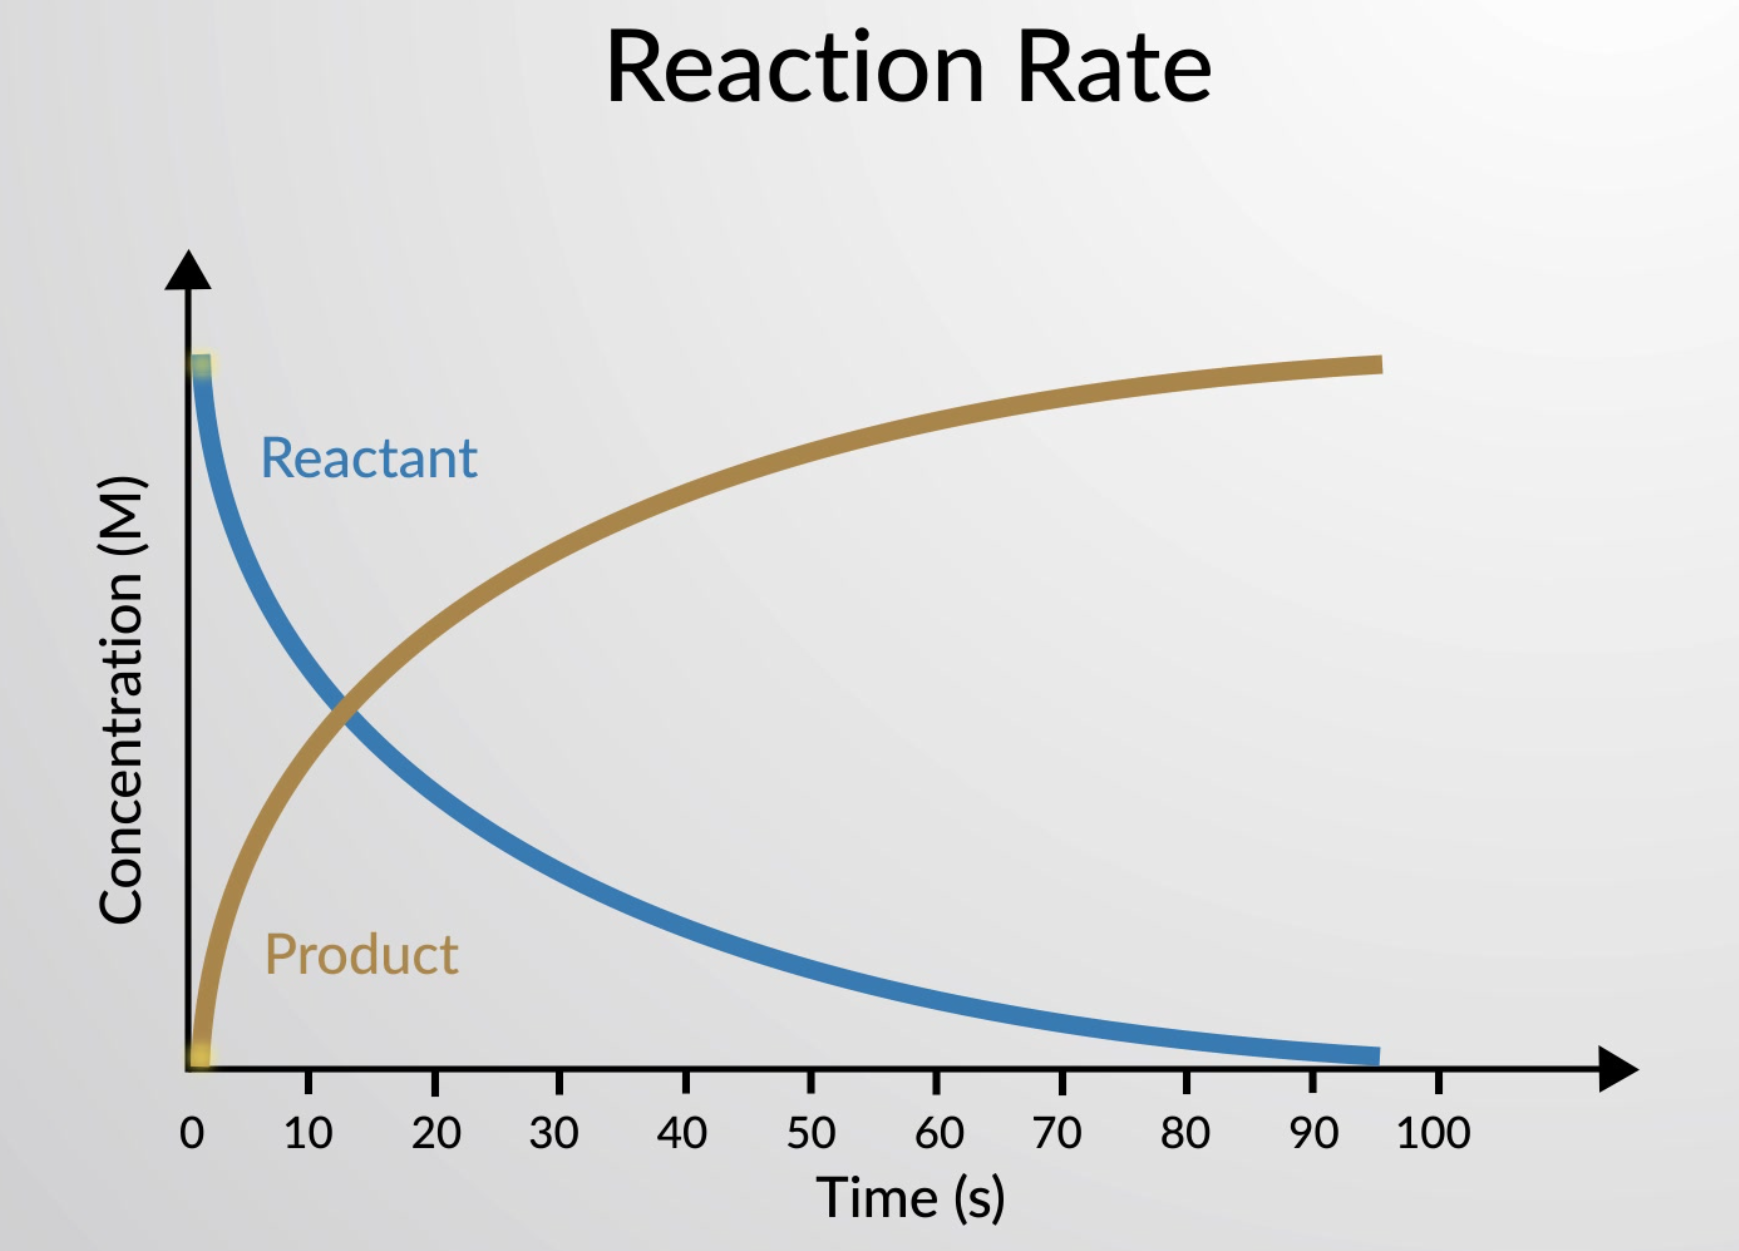
\includegraphics[height=0.35\columnwidth]{figures/chemical-kinetics/chemical-kinetics-intro}
	\end{figure}
\end{frame}
%
% --------------------------------------------------------------------------------------------------------------------%
% Application of kinetic reactions
% --------------------------------------------------------------------------------------------------------------------%
%
\begin{frame}{Application of kinetic reactions}
	
 \alert{\bf Reaction mechanisms} are used in many fields of science and technology: 

%\vskip -10pt
\lcol
{
\begin{itemize}
	\item combustion (turbulent combustion modeling),
	\item atmospheric chemistry,
	\item environmental/ecological modeling (e.g., Lotka--Volterra model describing the dynamics of the biological predator–prey interactions model), 
	\item process engineering, and 
	\item systems biology (with biological and biochemical processes such as cell cycle, metabolism networks and molecular signal transfer).
\end{itemize}
}

\rcol

\begin{figure}
	\vskip 10pt
	\centering
	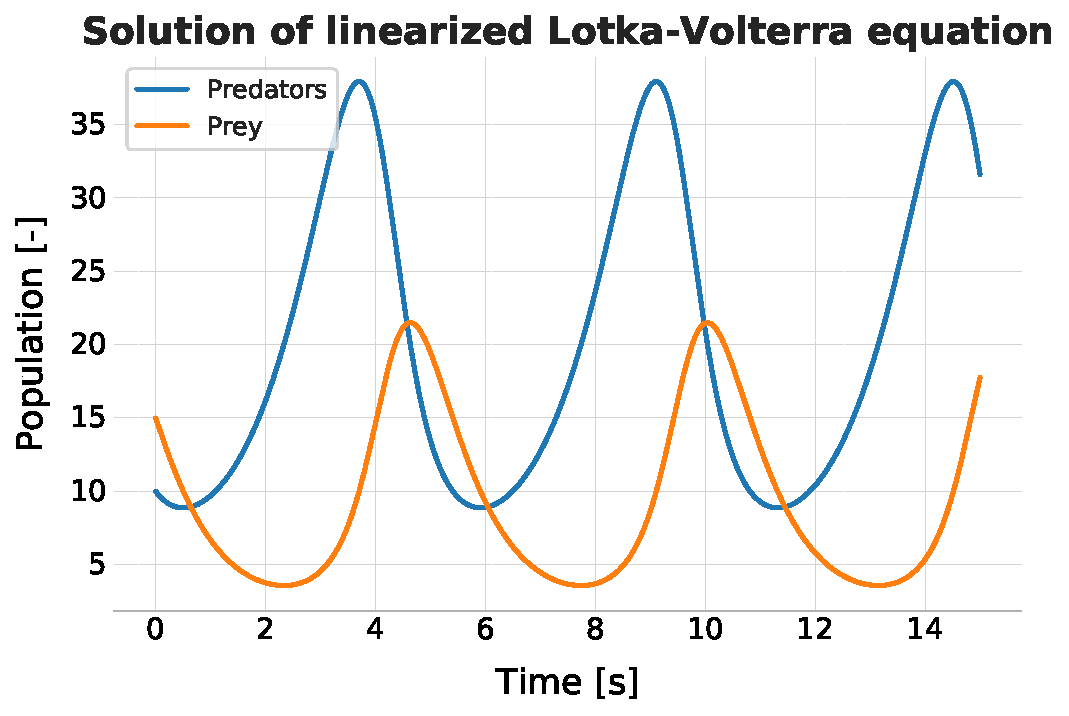
\includegraphics[height=0.6\columnwidth]{figures/chemical-kinetics/lotka-volterra}
	%\caption{Periodic solutions of the linearized the Lotka--Volterra equation.}
\end{figure}

\ecol
\end{frame}
%
% --------------------------------------------------------------------------------------------------------------------%
% Global and elementary chemical kinetics reaction
% --------------------------------------------------------------------------------------------------------------------%
%
\begin{frame}[<+->][shrink]{Global and elementary chemical kinetics reaction}
	
	\begin{itemize}
		\item Quite often kinetic mechanisms are described in a \textbf{single global step}. 
		\item \textbf{But!} In reality, such reaction happen in a series of elementary steps, \textbf{sequence of one or more
			elementary reactions}:
		\begin{itemize}
			\item {\it unimolecular reaction}: dissociation of one reagent molecule;
			\item {\it bimolecular reaction}: collisions between two molecules; or
			\item{ \it trimolecular reaction}: collision of three reactant molecules (occurs less frequently).
		\end{itemize}
		\item \alert{\textbf{Elementary chemical reactions}} is a transition between two atomic / molecular states. 
		%
		$$\mbox{State A} \xrightarrow[]{\text{Activation Energy}, \;E_a} \mbox{State B}$$
		%
		\item The \textbf{activation energy} between these two states determines \alert{the rate at which reactions occur}: 
		%
		\begin{itemize}
			\item for \it{low activation energy} $\Rightarrow$ reaction is rapid, 
			\item for \it{higher activation energy} $\Rightarrow$ reaction is slower.
		\end{itemize}
		%
	\end{itemize}
	
\end{frame}
%
% --------------------------------------------------------------------------------------------------------------------%
% Factors affecting reaction rates
% --------------------------------------------------------------------------------------------------------------------%
%
\begin{frame}[<+->]{Factors affecting reaction rates}
	
	\begin{itemize}
		\item {\bf Nature of the reactants} (strength of bonds, size of the product)
		\item {\bf Physical state} (solid, gas, or liquid phase)
		\item {\bf Surface area of solid state} (surface that can be involved in a reaction)
		\item {\bf Concentration} (higher the concentration $\Rightarrow$ higher the rate of reaction)
		\item {\bf Temperature} (higher the temperature $\Rightarrow$ higher the molecule thermal energy $\Rightarrow$ higher )
		\item {\bf Catalysts}, a substance that alters the rate of a chemical reaction but remains unchanged itself (increases the rate of the reaction)
		\item {\bf Pressure} (higher the pressure $\Rightarrow$ higher the number of collisions between reactants $\Rightarrow$ higher the rate of reaction)
		\item {\bf Absorption of light} (light absorption provide activation energy)
		%
	\end{itemize}
	
\end{frame}
%
% --------------------------------------------------------------------------------------------------------------------%
% Time scale of kinetics reactions, Examples
% --------------------------------------------------------------------------------------------------------------------%
%
\begin{frame}[<+->]{Time scale of kinetics reactions, Examples}
	\small
	\begin{itemize}
		%
		\item \textbf{\alert{The time scale}}, on which the chemical reactions occur, spans many orders of magnitude (from microseconds to years).
		%
		\item Reactions are characterized by the so-called  \textbf{\alert{half-time}} (dependent on the nature and the order of reaction).
		%
		\item The range of time scales can differ by several orders of magnitude:
		
		\begin{itemize}
			\item[$\bullet$]
			\[\mathsf{H_2CO_3(aq) \rightleftharpoons H^+ + HCO_3^-}\] 
			is acid–base reaction involving only solutes has \textbf{half-time of about $10^{-6}$ s}
			%
			\item[$\bullet$]
			\[\mathsf{CO_2(aq) + H_2O(l) \rightleftharpoons H_2CO_3(aq)}\] 
			is a solute–water hydration reaction has a \textbf{half-time of 0.1 s}
			
			\item[$\bullet$]
			\[\mathsf{CaCO_3(s, calcite) + H^{+} \rightleftharpoons Ca^{2+} + HCO_3^{-}}\] 
			mineral dissolution reaction can be in the\textbf{ order of weeks at low temperatures}
		\end{itemize}
	\end{itemize}
	
\end{frame}
%
% --------------------------------------------------------------------------------------------------------------------%
% Half-times of some reactions
% --------------------------------------------------------------------------------------------------------------------%
%
\begin{frame}{Half-times of some reactions}
	\begin{center}
		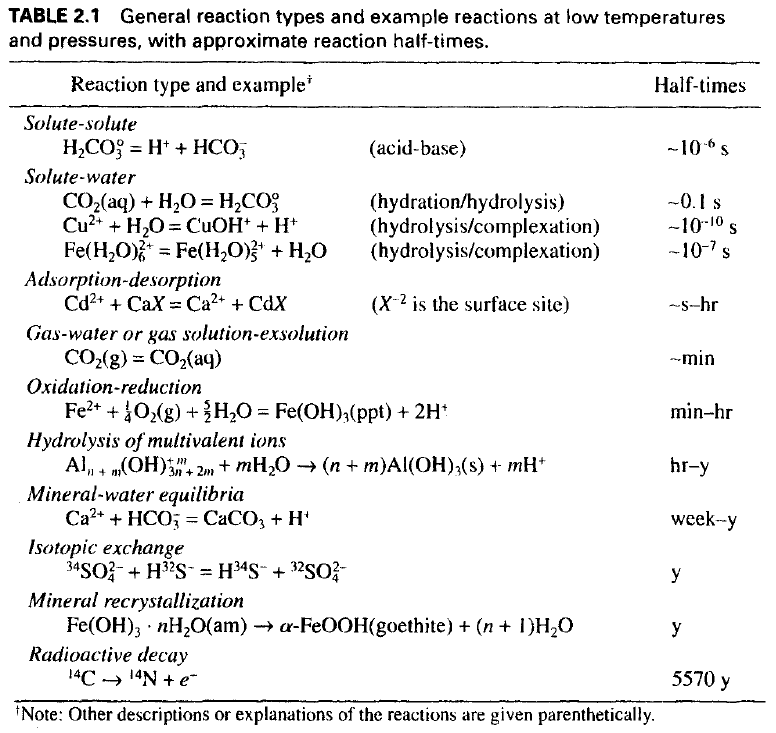
\includegraphics[height=0.85\textheight]{figures/reactive-transport/langmuir-reaction-half-times}{\scriptsize{}}\\
		{\tiny{}Langmuir, D., Aqueous Environmental Geochemistry, Prentice
			Hall, 1997}{\tiny\par}
		\par\end{center}
	
\end{frame}
%
\subsection{Reaction stoichiometry, rates, and orders}
%
% --------------------------------------------------------------------------------------------------------------------%
% Reaction stoichiometry
% --------------------------------------------------------------------------------------------------------------------%
%
\begin{frame}[<+->]{Reaction stoichiometry}
%
\vskip 5pt
\small
\begin{itemize}
	\item Chemical process can be described by the \alert{\textbf{single stoichiometric equation}}, also called  \alert{\textbf{overall reaction equation}}. 
	\item \alert{\textbf{Stoichiometric equation}} defines the molar ratio of the reacting species and the reaction products / the number of moles of each reactant and the product that appears in the overall reaction equation.
	\item {\bf Example}: the overall reaction equation for the \alert{combustion (oxidation) of hydrogen}: %/ water production:
	%
	\[\mathsf{2 H_2 + O_2 \rightleftharpoons 2H_2O},\] 
	%	
	where $\mathsf{H_2}$ has stoichiometric coefficient 2, 
	$\mathsf{O_2}$ has coefficient 1, 
	and $\mathsf{H_2O}$ has coefficient 2.
	%
	\item Chemical systems described by a single chemical reaction (reactants $\rightarrow$ products) are {\bf very rare}. 
	\item In reality, we are dealing with a network of {\bf elementary reactions}
	%
	\begin{multline*}
		\mbox{reactants} 
		\xrightarrow[]{\text{elem. react. 1}} \mbox{intermetiade 1} \xrightarrow[]{\text{elem. react. 2}} \ldots \\
		\xrightarrow[]{\text{elem. react i}} \mbox{intermetiade i} \xrightarrow[]{\text{elem. react. i+1}} \ldots \xrightarrow[]{\text{elem. react. N}} \mbox{products}
	\end{multline*}
	%
\end{itemize}
%
\end{frame}
%
% --------------------------------------------------------------------------------------------------------------------%
% Reaction stoichiometry, generalization
% --------------------------------------------------------------------------------------------------------------------%
%
\begin{frame}{Reaction stoichiometry, generalization}
	%
	\footnotesize
	\vskip 5pt
	\begin{itemize}
		\item Equation $\mathsf{2 H_2 + O_2 \rightleftharpoons 2H_2O}$ can be rearranged as follows
		%	
	    \[\mathsf{0 = - 2 H_2 - O_2 + 2H_2O},\] 
	    %
	    \vskip -5pt
	    \pause
	    \item If $ \mathsf{A = (A_1, A_2, A_3) =(H_2, O_2, H_2O)}$ is a vector of species, and 
	     $\mathsf{\nu = (\nu_1, \nu_2, \nu_3) = (-2, -1, 2)}$ is a vector of multiplication factors, 
	     then we obtain
	     %
	    \[0 = \sum_{i=1}^{3} \nu_i \,  \mathsf{A_i}.\]
	    \vskip -5pt
	    \pause
		\item The \alert{\textbf{general stoichiometric equation of chemical reaction}} is defined by
		%
		\[\boxed{0 = \sum_{i=1}^{N} \nu_i \, A_i,}\]
		\vskip -5pt
		%
		where 
			\begin{itemize}
			\item $N$ is the number of species, 
			\item $\nu_i$ is the stoichiometric coefficient of the $i$th species 
			($\nu_i < 0$ for reactants and $\nu_i >0$ for products), and 
		    \item  $ \mathsf{A_i}$ is s the formula of the $i$th species in the overall reaction equation.
	    	\end{itemize}
	%
	\end{itemize}
	%
\end{frame}
%
% --------------------------------------------------------------------------------------------------------------------%
% Complexity of finding single overall reaction equation
% --------------------------------------------------------------------------------------------------------------------%
%
\begin{frame}[<+->]{Complexity of finding single overall reaction equation}
	%
	\small
	There are {\bf many chemical processes} for which a {\bf single overall reaction equation}
	that describes the stoichiometry of the process \alert{{\bf cannot be found}}.
	%
	\lcol
		\begin{itemize}
		\item {\bf Example}: \alert{oxidation of hydrocarbons sourced from exhaust gases in the troposphere}, 
		with the sequence of reactions \\[5pt]
		{
			\scriptsize
			$\bullet$ hydrocarbon + OH $\rightarrow$ alkyl radical + H$_2$O, \\[3pt]
			$\bullet$ alkyl radical + O$_2$ ($^3\sum$) $\rightarrow$ alkylperoxy radical, \\[3pt]
			$\bullet$ alkylperoxy radical + NO $\rightarrow$ alkoxy radical + NO$_2$, \\[3pt]
			$\bullet$ alkoxy radical + O$_2$($^3\sum$) $\rightarrow$ aldehyde + HO. \\[10pt]
		}
		%
		\item The atmospheric {\bf lifetimes of hydrocarbons} are determined by their {\bf reactivity towards OH} as well as by the {\bf average OH concentration level} $\Rightarrow$ these lifetimes {\bf vary from several hours to several years}.
		\end{itemize}

	
	\rcol
	
	\begin{figure}
		\vskip 5pt
		\centering
		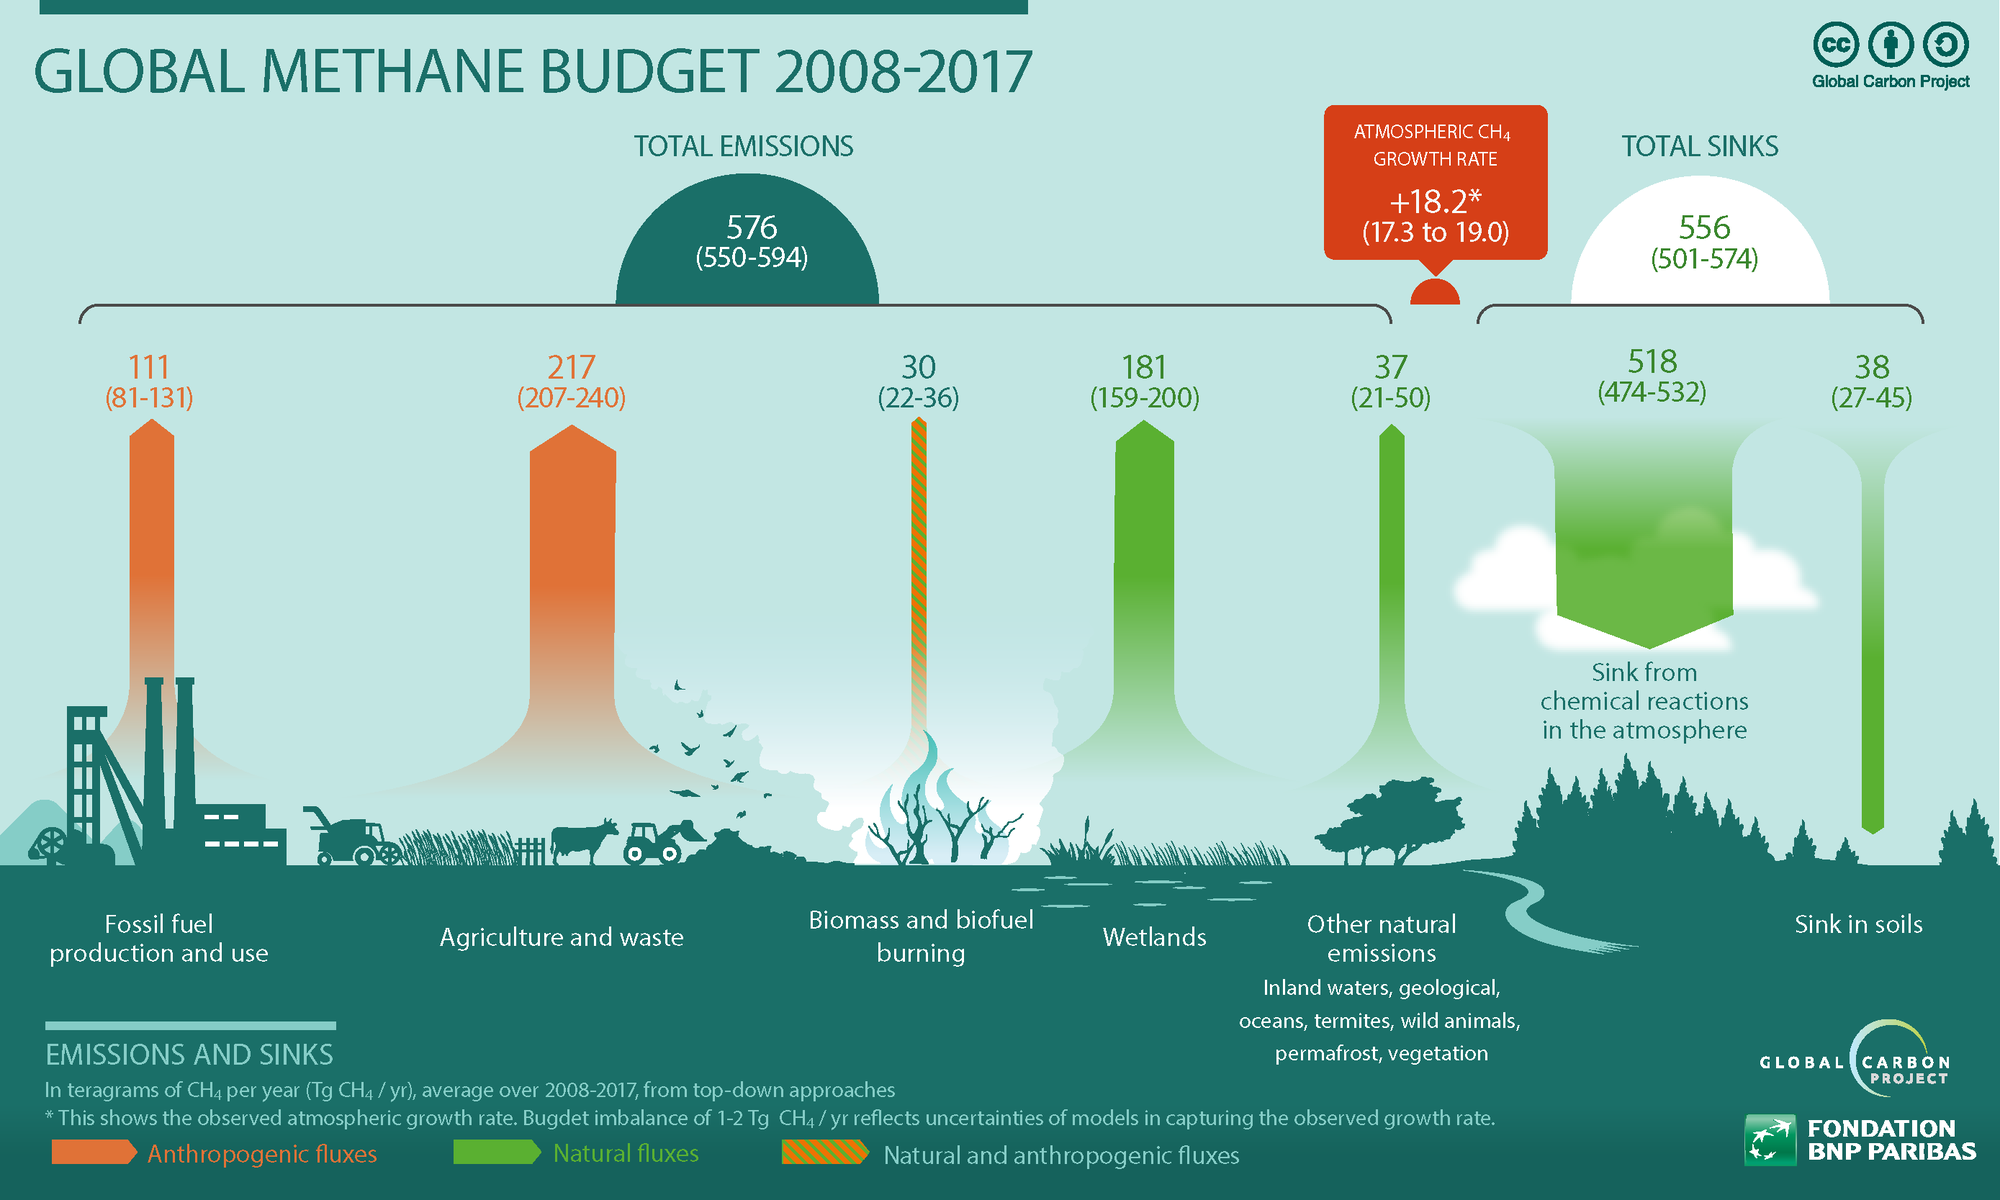
\includegraphics[height=0.5\columnwidth]{figures/chemical-kinetics/methane-sources.png}
		\caption{Diagram showing the main sources of methane for the decade 2008-2017, 
			produced by a global report on global methane emissions by the Global Carbon Project 
			(source \href{https://en.wikipedia.org/wiki/Atmospheric_methane}{\textcolor{indigo(dye)}{\tt Wikipedia}}).}
	\end{figure}
	
	\ecol
\end{frame}
%
% --------------------------------------------------------------------------------------------------------------------%
% Reaction rate as production/consumption rate
% --------------------------------------------------------------------------------------------------------------------%
%
\begin{frame}{Reaction rate as production/consumption rate}
	\small 
%	
\begin{itemize}
	\item \textbf{\alert{The reaction rate}} is the rate at which reactants are consumed, 
		or the rate at which products are formed, 
		%$\mathsf{\frac{mol}{s}}$.
		$\mathsf{\frac{mol}{m^3 \cdot s}}$.
	\pause
	\item The reaction rate can be defined as \textbf{\alert{the rate of change of concentration}} of a
reactant/product divided by its stoichiometric coefficient. 
\end{itemize}
%
\lcol
{
	\small
	\begin{itemize}
		\pause
		\item {\bf Example}: for hydrogen oxidation 
		%
		$\mathsf{2 \,H_2 + O_2 \rightleftharpoons 2\, H_2O},$
		%
		the reaction rate is defined as
		%
		\[r = \tfrac{1}{2}  \tfrac{d \mathsf{[H_2O]}}{dt} = \alert{-} \tfrac{1}{2}  \tfrac{d \mathsf{[H_2]}}{dt} = \alert{-}\tfrac{d \mathsf{[O_2]}}{dt}.\] 
		\vskip -10pt
		%
		\pause
		\item For more \textbf{\alert{general reaction}} $0 \rightleftharpoons \sum_{i=1}^{N} \nu_i \,  \mathsf{A_i}$, 
		%
		we obtain
		% 
		\[\boxed{ r = \tfrac{1}{\nu_i}  \tfrac{d [ \mathsf{A_i}]}{dt}.}\] 
	\end{itemize}
}
\rcol
%
\vskip -20pt
\begin{figure}[th]
	    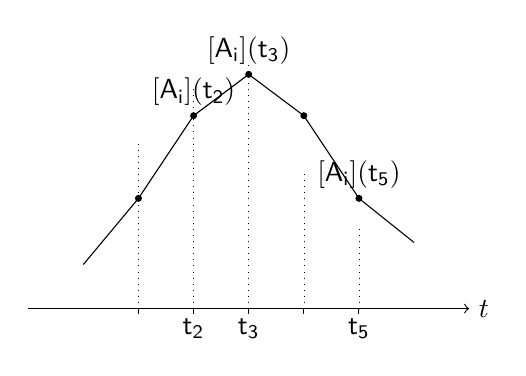
\begin{tikzpicture}[scale=0.7]
			
			\draw[->] (-1,0) -- (7,0) node[anchor=west] {$t$}; % t-axis
			
			% vertical lines
			\draw[line width=0.2pt,dotted] (1,0) -- (1,3);
			\draw[line width=0.2pt,dotted] (2,0) -- (2,4);
			\draw[line width=0.2pt,dotted] (3,0) -- (3,4.5);
			\draw[line width=0.2pt,dotted] (4,0) -- (4,2.5);
			\draw[line width=0.2pt,dotted] (5,0) -- (5,1.5);
			
			% draw ticks
			\foreach \x in {1,2,3,4,5}
			\draw (\x,0) -- (\x,-0.1);
			
			% averaged function
			\draw[line width=0.4pt] (0,0.8) -- (1,2);
			\draw[line width=0.4pt] (1,2) -- (2,3.5);
			\draw[line width=0.4pt] (2,3.5) -- (3,4.25);
			\draw[line width=0.4pt] (3,4.25) -- (4,3.5);
			\draw[line width=0.4pt] (4,3.5) -- (5,2);
			\draw[line width=0.4pt] (5,2) -- (6,1.2);
			
			\filldraw [black] (1,2) circle (1.5pt);
			\filldraw [black] (2,3.5) node[anchor=south] {$\mathsf{[A_i](t_2)}$} circle (1.5pt);
			\filldraw [black] (3,4.25) node[anchor=south] {$\mathsf{[A_i](t_3)}$} circle (1.5pt);
			\filldraw [black] (4,3.5) circle (1.5pt);
			\filldraw [black] (5,2) node[anchor=south] {$\mathsf{[A_i](t_5)}$} circle circle (1.5pt);]
			
			% time marks
			\filldraw [black] (2,0) node[anchor=north] {$\mathsf{t_2}$} circle (0.1pt);
			\filldraw [black] (3,0) node[anchor=north] {$\mathsf{t_3}$} circle (0.1pt);
		    \filldraw [black] (5,0) node[anchor=north] {$\mathsf{t_5}$} circle (0.1pt);
			
		\end{tikzpicture}
	\caption{Time-dependent behaviour of the chemical system: the molar concentrations of species $\mathsf{A_i}$ measured at consecutive time points.}
	\end{figure}
\ecol
%
\end{frame}

\begin{frame}{Quiz, Production/consumption rate}
	
	\begin{itemize}
		\item Consider the reaction 
		%
		$$\mathsf{a\, A + b\, B \rightleftharpoons c \, C + d \, D}.$$
		%
		\item Knowing that $r = \tfrac{1}{\nu_i}  \, \tfrac{d [ \mathsf{A_i}]}{dt} = \tfrac{1}{\nu_i} \, r(\mathsf{A_i}),$ where $\nu_i > 0$ for products and $\nu_i < 0$ for reactants. 
		%
		\pause
		\alert{\bf Quiz} (multiple choice): which statements about reaction/production rates are correct?
		%
		\vskip 5pt
		\begin{center}
    	\href{http://etc.ch/wsKw}{\textcolor{indigo(dye)}{\tt http://etc.ch/wsKw}} \quad
			or 
		    \quad	
\includegraphics[height=0.12\columnwidth]{figures/chemical-kinetics/polls.png}
		\end{center}
		\hiddenpause 
		\vskip 10pt
		\item \alert{\bf Answer}: the correct relations on the reaction/production rates are
		%
		\begin{alignat*}{2}
		- \tfrac{1}{a} \, r(\mathsf{A}) & = \tfrac{1}{d}\,  r(\mathsf{D}) \quad \Rightarrow \quad r(\mathsf{A}) = - \tfrac{a}{d} \,  r(\mathsf{D}), \\[-3pt]
		- \tfrac{1}{b} \, r(\mathsf{B}) &  = \tfrac{1}{d} \,  r(\mathsf{D}), \\[-3pt]
		\tfrac{1}{c} \,  r(\mathsf{C})  & = \tfrac{1}{d} \,  r(\mathsf{D}) \quad \Rightarrow \quad r(\mathsf{C}) = \tfrac{c}{d} \,  r(\mathsf{D}).
		\end{alignat*}	
	\end{itemize}
\end{frame}
%
% --------------------------------------------------------------------------------------------------------------------%
% Reaction rate via concantrations of reactants
% --------------------------------------------------------------------------------------------------------------------%
%
\begin{frame}[shrink]{Reaction rate via concentrations of reactants}
%
\begin{itemize}
\item \alert{\bf Reaction rate for general equation}
%
\[0 \rightleftharpoons \sum_{i=1}^{N} \nu_i \, \mathsf{A_i},\]
%
can be defined {\bf proportional to the concentrations of the reactants raised to a power}:
%
\[r := k \prod_{i=1}^{N} [\mathsf{A_i}]^{\alpha_i},\]
%
where
%
\begin{itemize}
	\item $k > 0$ is the {\bf rate coefficient}, 
	\item $[\mathsf{A_i}]$ is a molar concentrations ($\mathsf{\tfrac{mol}{m^3}}$), 
	\item $\alpha_i > 0$ is the {\bf order of reaction with respect to species $\mathsf{A_i}$}, %such that $\alpha := \sum_{i}^{N} \alpha_i$ is the overall order of reaction, 
	and 
	\item $N$ is the number of species.
\end{itemize}
%
\end{itemize}
%
\end{frame}
%
\begin{frame}{Quiz, Reaction rate via concentration of reactants}
	
	\begin{itemize}
		\item Consider the elementary reaction 
		%
		$$\mathsf{a\, A + b\, B \rightleftharpoons c \, C + d \, D}.$$
		%
		\item 
		\alert{\bf Quiz}: what is the reaction rate of this reaction?
		%
		\vskip 5pt
		\begin{center}
    	\href{http://etc.ch/wsKw}{\textcolor{indigo(dye)}{\tt http://etc.ch/wsKw}} \quad
			or 
		    \quad	
\includegraphics[height=0.12\columnwidth]{figures/chemical-kinetics/polls.png}
		\end{center}
		%
		\hiddenpause 
		\vskip 10pt
 		\item \alert{\bf Answer}: the correct reaction rate is 
 		$\mathsf{r = k {[A]}^a {[B]}^b}$.
	\end{itemize}
\end{frame}
% --------------------------------------------------------------------------------------------------------------------%
% Order of reaction vs. stoichiometry
% --------------------------------------------------------------------------------------------------------------------%
%
\begin{frame}{Order of reaction vs. stoichiometry}
	%
	\small
	\begin{itemize}
	\item The sum of the powers is \alert{\bf the overall order of the reaction}, i.e., 
	%
	\[\mathsf{\alpha = \sum_{i=1}^{N} \alpha_i}.\]
	%
	\pause
	\item For the overall reaction equation, \alert{\bf the order does not necessarily reflect the stoichiometry}, i.e., 
	%
	$\alpha_i \neq \nu_i$,
	%
	because of the {\bf intermediate steps} hidden in the overall reaction.\\[5pt]
	%
	{\bf Example}: in the reaction $\mathsf{CO + Cl_2 \xrightleftharpoons[]{r} COCl_2}$, the reaction rate $r = \mathsf{[CO]^2 \cdot [Cl_2]^{3/2}}$.
	%
%	\begin{itemize}
%		\item for $\mathsf{2\,NO + O_2 \xrightleftharpoons[]{k} 2\,NO_2}$: $k = \mathsf{[NO]^2 \cdot [O_2]}$;
%	    \item for $\mathsf{CO + Cl_2 \xrightleftharpoons[]{k} COCl_2}$: $k = \mathsf{[CO]^2 \cdot [Cl_2]^{3/2}}$.
%    \end{itemize}
	%
	\pause
	\vskip -5pt
	\pause
	\item For elementary reactions, {\bf the reaction orders and the absolute value of the stoichiometric
coefficients} of the reactants are \alert{\bf commonly the same}. \\[5pt]
%
    {\bf Example}:
	\begin{itemize}
	\item for unimolecular decomposition $\mathsf{A \xrightleftharpoons[]{r} B}$: $r = \mathsf{[A]}$
	%
	\item for bimolecular reaction \\[5pt]
 	$\bullet$ $\mathsf{A + B \xrightleftharpoons[]{r} C}$: $r = \mathsf{[A] \cdot [B]}$, or \\
	$\bullet$ $\mathsf{A + A \xrightleftharpoons[]{r} C}$: $r = \mathsf{[A]^2}$.
	\end{itemize}
\end{itemize}
	%
\end{frame}
%
\begin{frame}{Quiz, Order of reaction}
	
	\begin{itemize}
		\item Consider the reaction 
		%
		$$\mathsf{
		C_{6}H_{5}N_{2}Cl(aq) + H_{2}O (l) 
        \rightleftharpoons
        C_{6}H_{5}OH(aq) + N_{2}(g) + HCl(aq)}.$$
		%
		\item 
		\alert{\bf Quiz}: given that $\mathsf{r = k [C_{6}H_{5}N_{2}Cl(aq)]^1 [H_{2}O(l)]^0}$, what is the overall order of this reaction?
		%
		\vskip 5pt
		\begin{center}
    	\href{http://etc.ch/wsKw}{\textcolor{indigo(dye)}{\tt http://etc.ch/wsKw}} \quad
			or 
		    \quad	
\includegraphics[height=0.12\columnwidth]{figures/chemical-kinetics/polls.png}
		\end{center}
		%
		\hiddenpause 
		\vskip 10pt
 		\item \alert{\bf Answer}: the overall order is 1.
	\end{itemize}
\end{frame}
% --------------------------------------------------------------------------------------------------------------------%
% Stoichometry in intermediate reactions
% --------------------------------------------------------------------------------------------------------------------%
%
\begin{frame}{Stoichiometry in intermediate reactions}
	%
	\small
	\begin{itemize}
		\item 
	The overall \alert{\bf reaction of hydrogen combustion} $\mathsf{2 \, H_2 + O_2 \rightleftharpoons 2\, H_2O}$ should contain the following intermediate steps (among total 30-40 steps):
	{\small
		\lcol
		\begin{alignat*}{2}
			R_1:  & \quad \mathsf{H_2 + O_2 \xrightleftharpoons[]{k_1} H + HO_2} \\
			R_2: & \quad \mathsf{O_2 + H \xrightleftharpoons[]{k_2} OH + O} \\
			R_3: & \quad \mathsf{H_2 + OH \xrightleftharpoons[]{k_3} H + H_2O} \\
		\end{alignat*}
	  \rcol
	  \vskip -30pt
	  \begin{alignat*}{2}
	  	R_4: & \quad \mathsf{H_2 + O \xrightleftharpoons[]{k_4} H + OH} \\
	  	R_5: & \quad \mathsf{O_2 + H + M \xrightleftharpoons[]{k_5} HO_2 + M} \\
	  	R_6: & \quad \mathsf{HO_2 + OH \xrightleftharpoons[]{k_6} H_2O + OH}.
	  \end{alignat*}
	  \ecol
	}
	%where $M$ is any species present in the mixture.
	%
	\pause
	\item Each {\bf elementary reaction step $j$} can be characterized by the stoichiometric equation
	%
	\[
	\sum_{i} \nu^R_{ji}	\mathsf{A_i} \xrightleftharpoons[]{k_j} \sum_{i} \nu^P_{ji} \mathsf{A_i}
	\]
	%
	\vskip -10pt
	\pause
	\item The \alert{\bf stoichiometric coefficient belonging to species $\mathsf{A_i}$ in a reaction step $j$} can be calculated by
	%
	\[
	\nu_{ji} = \nu^P_{ji} - \nu^R_{ji}.
	\]
\end{itemize}
	%
\end{frame}
%
% --------------------------------------------------------------------------------------------------------------------%
% Differential \& integral forms for the reaction rate, Half-time
% --------------------------------------------------------------------------------------------------------------------%
%
\begin{frame}[<+->]{Differential \& integral forms for the reaction rate, Half-time}
%
\footnotesize
\begin{itemize}
	\item To establish the relationship between the {\bf rate of change of the concentration of a reactant/product}  and  {\bf reaction rate} over time, i.e., 
	$$r := \tfrac{1}{\nu_i}  \, \tfrac{d [ \mathsf{A_i}]}{dt} \quad \mbox{and} \quad 
		r := k \prod_{i=1}^{N} [\mathsf{A_i}]^{\alpha_i},$$
	the {\bf differential equation} is used.
	\item For simple cases, it may be analytically integrated (see Table \ref{tab:differential-integral-forms}) to obtain \alert{\bf the integral form}.
	\item \alert{\bf The half-life of the reaction} is the time required for the reagent concentration be reduced to half of its initial
value.
\end{itemize}
\begin{table}
\footnotesize
	\begin{tabular*}{1\textwidth}{@{\extracolsep{\fill}}lcccc}
		\toprule 
		Reaction & Order & Differential Form & Integrated form & Half-time \\[5pt]
		\midrule 
		A $\rightarrow$ B & 0 & $-\tfrac{d \mathsf{[A]}}{dt} = k_0$ & $\mathsf{[A]} = \mathsf{[A]_0} - k_0\,t$ & 
		$t_{1/2} = \tfrac{\mathsf{[A]_0}}{2\,k_0}$ \\[5pt]
		A $\rightarrow$ B + C & 1 & $-\tfrac{d \mathsf{[A]}}{dt} = k_1\, \mathsf{[A]}$ & $\ln \mathsf{[A]} = \ln \mathsf{[A]_0} - k_1\,t$ & $t_{1/2} = \tfrac{\ln 2}{k_1}$ \\[5pt]
		A + B  $\rightarrow$ C & 2 & $-\tfrac{d \mathsf{[A]}}{dt} = k_2\, \mathsf{[A]}\, \mathsf{[B]}$ & 
		$k_2\,t = \tfrac{1}{\mathsf{[B]_0} + \mathsf{[A]_0}} \ln \tfrac{\mathsf{[B]_0} \mathsf{[A]}}{\mathsf{[B]} \mathsf{[A]_0}}$ & $t_{1/2} = \tfrac{1}{k_2 \, \mathsf{[A]_0}}$ (B = A) \\[5pt]
		\bottomrule
	\end{tabular*}
	%
	\caption{\label{tab:differential-integral-forms} \footnotesize Differential and integral forms for the reaction rate as well as half-time, where $\mathsf{[A]_0}$ and $\mathsf{[B]_0}$ correspond to the initial concentrations of A and B, respectively.}
\end{table}
%
\end{frame}
%
% --------------------------------------------------------------------------------------------------------------------%
% Example, Differential \& integral forms for the reaction rate, Half-time
% --------------------------------------------------------------------------------------------------------------------%
%
\begin{frame}{Quiz, Differential \& integral forms for the reaction rate, Half-time}
	%
	\begin{itemize}
		\item \alert{\bf Quiz}: Given a first-order reactant and rate constant  $k_1$ = 1.5e-4 1/min, what is the the half-life of the reactant if the time is defined by  $t_{1/2} = \tfrac{\ln 2}{k_1}$?
		%
		\begin{center}
			\href{http://etc.ch/wsKw}{\textcolor{indigo(dye)}{\tt http://etc.ch/wsKw}} 
			\quad or \quad  
			
\includegraphics[height=0.2\columnwidth]{figures/chemical-kinetics/polls.png}
		\end{center}
 		\hiddenpause 
 		\vskip 10pt
 		\item {\bf Answer}: ln(2) / 1.5e-4 min = 
 		ln2 / 0.0000025 s $\approx$ 27.73e4 s
	\end{itemize}
	%
\end{frame}
%
\begin{frame}{Quiz, Reaction rate for the different order reactions}
	%
	\begin{itemize}
		\item \alert{\bf Quiz} (multi-choice): Knowing formulation of the reactions rate for different order reactions
		
		\begin{table}
\footnotesize
	\begin{tabular*}{1\textwidth}{@{\extracolsep{\fill}}lcccc}
		\toprule 
		Reaction & Order & Differential Form & Integrated form & Half-time \\[5pt]
		\midrule 
		A $\rightarrow$ B & 0 & $-\tfrac{d \mathsf{[A]}}{dt} = k_0$ & $\mathsf{[A]} = \mathsf{[A]_0} - k_0\,t$ & 
		$t_{1/2} = \tfrac{\mathsf{[A]_0}}{2\,k_0}$ \\[5pt]
		A $\rightarrow$ B + C & 1 & $-\tfrac{d \mathsf{[A]}}{dt} = k_1\, \mathsf{[A]}$ & $\ln \mathsf{[A]} = \ln \mathsf{[A]_0} - k_1\,t$ & $t_{1/2} = \tfrac{\ln 2}{k_1}$ \\[5pt]
		A + B  $\rightarrow$ C & 2 & $-\tfrac{d \mathsf{[A]}}{dt} = k_2\, \mathsf{[A]}\, \mathsf{[B]}$ & 
		$k_2\,t = \tfrac{1}{\mathsf{[B]_0} + \mathsf{[A]_0}} \ln \tfrac{\mathsf{[B]_0} \mathsf{[A]}}{\mathsf{[B]} \mathsf{[A]_0}}$ & $t_{1/2} = \tfrac{1}{k_2 \, \mathsf{[A]_0}}$ (B = A) \\[5pt]
		\bottomrule
	\end{tabular*}
	%
\end{table}
		\vskip 10pt
		%
		Which statements below are correct?
		%
		\begin{center}
			\href{http://etc.ch/wsKw}{\textcolor{indigo(dye)}{\tt http://etc.ch/wsKw}} 
			\quad or \quad  
			
\includegraphics[height=0.1\columnwidth]{figures/chemical-kinetics/polls.png}
		\end{center}
		\hiddenpause 
		\vskip 10pt
		\item {\bf Answer}: Normally, the greater the concentration of reactants, the faster the reaction rate will occur. But this is not true of zero order reactions! 
	\end{itemize}
	%
\end{frame}
\begin{frame}
\centering
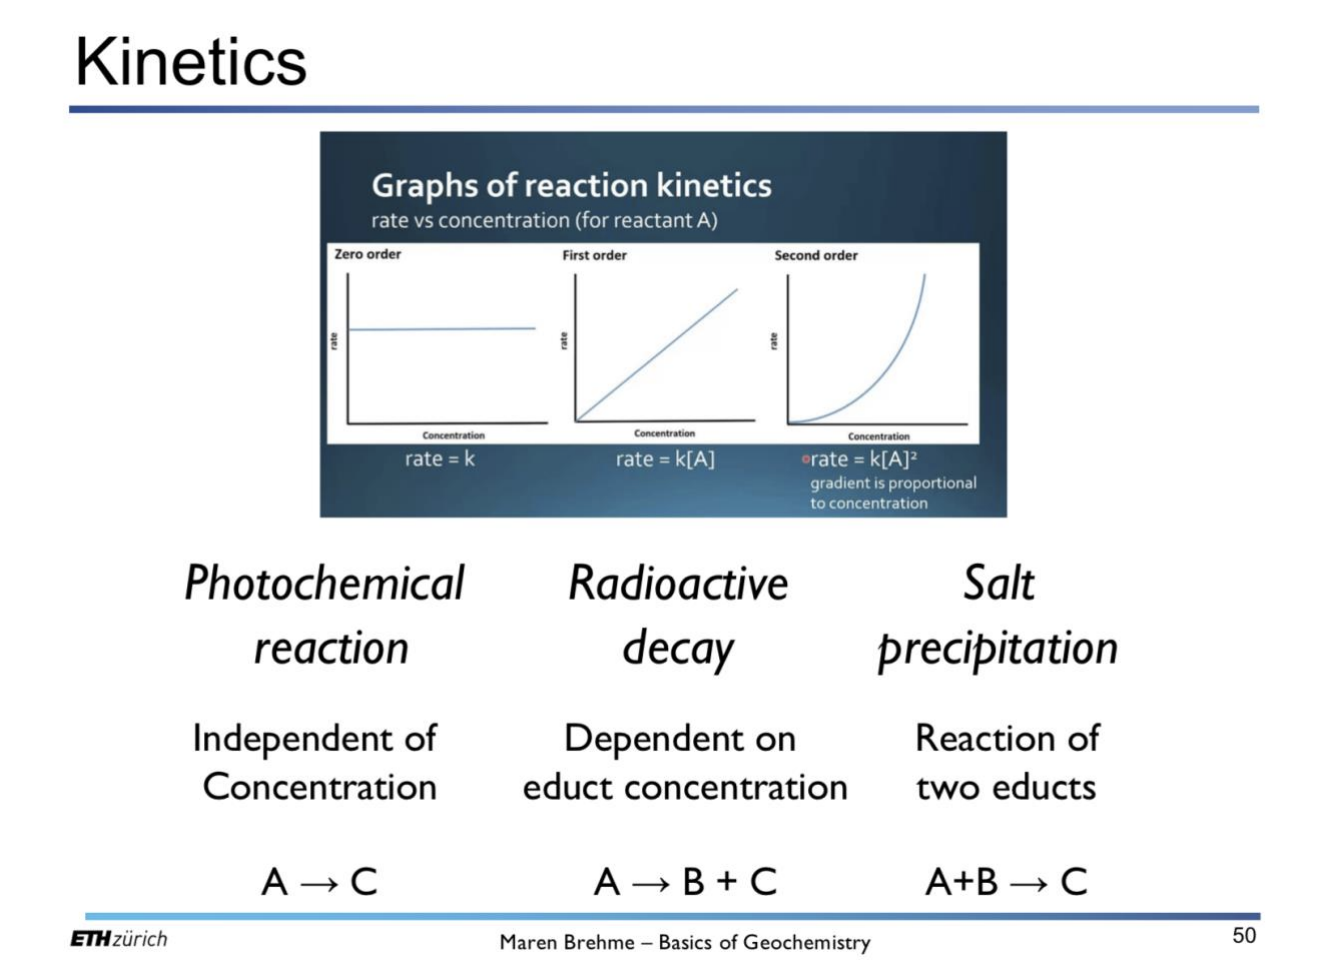
\includegraphics[height=0.6\textwidth]{figures/chemical-kinetics/maren-brener-slide.png}

\end{frame}
% --------------------------------------------------------------------------------------------------------------------%
% Mass action kinetics and corresponding kinetic system of ODEs
% --------------------------------------------------------------------------------------------------------------------%
%
\begin{frame}{Mass action kinetics and corresponding kinetic system of ODEs}
	%
	\footnotesize
	\begin{itemize}
		\item \alert{\bf The law of mass action kinetics} for elementary reactions can be formulated as
		%
		\[r_j := k_j \, \prod_{i=1}^{\mathsf{N}} \mathsf{[A_i]}^{\nu_{ji}}, \quad j = 1, \ldots, \mathsf{M}, \]
		\vskip -10pt
		%
		%
		where 
		\begin{itemize}
			\item $r_j $ is the kinetic rate of $j$th reaction step and $k_j$ is the $j$th rate coefficient, 
			\item $\mathsf{N}$ and $\mathsf{M}$ are the number of species and  the number of reactions, respectively, 
			\item $\nu_{ji}$ is the stoichiometric coefficient of the $i$th species, and 
			\item  $\mathsf{A_i}$ is the formula of the $i$th species, and $[\mathsf{A_i}]$ is its corresponding concentration.
		\end{itemize} 
	%
	\pause
	\item \alert{\bf Kinetic system of ordinary differential equations ODEs} defines the relationship between 
	{\bf production rates of the species} $\tfrac{d \mathsf{[A_i]}}{dt}$ and {\bf reaction rates} $r_j$:
	%
	\[
	\tfrac{d \mathsf{[A_i]}}{dt} = \sum_{j=1}^{\mathsf{M}} \nu_{ji} r_j, \quad i = 1, \ldots, \mathsf{N}.
	\]
	\vskip -5pt
	\pause
	\item The {\bf kinetic system of ODEs} and {\bf its initial values} together provide the following
	\alert{\bf initial value problem}
	%
	\[
	\tfrac{d \mathsf{[A_i]}}{dt} = \sum_{j=1}^{\mathsf{M}} \nu_{ji} r_j, 
	\quad [A_i](0) = [A_i]_0,
	\quad i = 1, \ldots, \mathsf{N}.
	\]
	\end{itemize}
	%
\end{frame}
%
% --------------------------------------------------------------------------------------------------------------------%
% Example: kinetics law of mass action for hydrogen combustion
% --------------------------------------------------------------------------------------------------------------------%
%
\begin{frame}{Example, Kinetics law of mass action for hydrogen combustion}
		\begin{itemize}
		\item The overall reaction $\mathsf{2 \, H_2 + O_2 \rightleftharpoons 2\, H_2O}$ can be 
		decomposed into the following $M=6$ elementary steps with corresponding 
		the stoichiometry matrix $\nu \in \mathbb{R}^{6 \times 8}$, $\nu = \{\nu_{i, j}\}_{i = 1, ...,6; j = 1, ..., 8}$
			\lcol
			{\scriptsize
			\begin{alignat*}{4}
				R_1:  & \quad \mathsf{H_2 + O_2 \xrightleftharpoons[]{k_1} H + HO_2}    & \quad & r_1 = k_1  \mathsf{[H_2][O_2] } \\[-5pt]
				R_2: & \quad \mathsf{O_2 + H \xrightleftharpoons[]{k_2} OH + O}           && r_2 = k_2  \mathsf{[O_2][H] } \\[-5pt]
				R_3: & \quad \mathsf{H_2 + OH \xrightleftharpoons[]{k_3} H + H_2O}     && r_3 = k_3  \mathsf{[H_2][OH] } \\[-5pt]
				R_4: & \quad \mathsf{H_2 + O \xrightleftharpoons[]{k_4} H + OH}           && r_4 = k_4  \mathsf{[H_2][O] } \\[-5pt]
				R_5: & \quad \mathsf{O_2 + H + M \xrightleftharpoons[]{k_5} HO_2 + M} && r_5 = k_5  \mathsf{[O_2][H][M] } \\[-5pt]
				R_6: & \quad \mathsf{HO_2 + OH \xrightleftharpoons[]{k_6} H_2O + O_2} && r_6 = k_6  \mathsf{[HO_2][OH] }
			\end{alignat*}
			}
			\rcol
			{\small
				\vskip -30pt
			\only<1	>{
			\vskip 15pt
			\[
			\nu = 
			\kbordermatrix{
				& \mathsf{H} & \mathsf{H_2} & \mathsf{HO_2} & \mathsf{H_2O} & \mathsf{O} & \mathsf{O_2} & \mathsf{OH} & \mathsf{M} \\
				R_1 &   1 & -1 & 1 & 0 & 0 & \alert{*} & 0 & 0\\[10pt]
				R_2 & -1 &  0 & 0 & 0 & 1 & \alert{*} & 1 & 0\\[10pt]
				R_3 &   1 & -1 & 0 & 1 & 0 & \alert{*} & -1 & 0\\[5pt]
				R_4 &  1 & -1 & 0 & 0 & -1 & \alert{*} & 1 & 0\\[5pt]
				R_5 & -1 &  0 & 1 & 0 & 0 & \alert{*} & 0 & 0\\[5pt]
				R_6 &  0 &  0 & -1 & 1 & 0 & \alert{*} & -1 & 0\\[5pt]
			}
			\]
			}
			\only<2>{
			\vskip 15pt
			\[
			\nu = 
			\kbordermatrix{
				& \mathsf{H} & \mathsf{H_2} & \mathsf{HO_2} & \mathsf{H_2O} & \mathsf{O} & \mathsf{O_2} & \mathsf{OH} & \mathsf{M} \\
				R_1 &   1 & -1 & 1 & 0 & 0 & \alert{-1} & 0 & 0\\[10pt]
				R_2 & -1 &  0 & 0 & 0 & 1 & \alert{-1} & 1 & 0\\[10pt]
				R_3 &   1 & -1 & 0 & 1 & 0 & \alert{0} & -1 & 0\\[5pt]
				R_4 &  1 & -1 & 0 & 0 & -1 & \alert{0} & 1 & 0\\[5pt]
				R_5 & -1 &  0 & 1 & 0 & 0 & \alert{-1} & 0 & 0\\[5pt]
				R_6 &  0 &  0 & -1 & 1 & 0 & \alert{1} & -1 & 0\\[5pt]
			}
			\]
			}
			}
			\ecol
	%
	\vskip 5pt 
	\item \alert{\bf Quiz}: What are the coefficients in the column with the O$_2$? \\[5pt]
	\begin{center}
		\href{http://etc.ch/wsKw}{\textcolor{indigo(dye)}{\tt http://etc.ch/wsKw}} \quad or \quad
		
\includegraphics[height=0.09\columnwidth]{figures/chemical-kinetics/polls.png}
	\end{center}
%	\item The production rates can be formulated as follows: 
%	{\footnotesize
%	\begin{alignat*}{2}
%		\tfrac{d\mathsf{H}}{dt} = & 1 \, r_1 - 1 \, r_2 + 1 \, r_3 + 1 \, r_4 -  1 \, r_5 + 0 \, r_6\\
%								  = &  k_1  \mathsf{[H_2][O_2] } - k_2  \mathsf{[O_2][H] } + k_3  \mathsf{[H_2][OH]}  + k_4  \mathsf{[H_2][O] } -  k_5  \mathsf{[H][O_2][M]} + 0 \, k_6  \mathsf{[HO_2][OH] }\\
%		\tfrac{d\mathsf{H_2O}}{dt} = & 1 \, r_3 + 1 \, r_6 
%		= k_3  \mathsf{[H_2][OH]} + k_6  \mathsf{[HO_2][OH] }\\
%	\end{alignat*}
%	}
	%
	\end{itemize}
\end{frame}
%
\begin{frame}{Example, Kinetics law of mass action for hydrogen combustion}
	\lcol
	{\scriptsize
		\begin{alignat*}{4}
			R_1:  & \quad \mathsf{H_2 + O_2 \xrightleftharpoons[]{k_1} H + HO_2}    & \quad & r_1 = k_1  \mathsf{[H_2][O_2] } \\[-5pt]
			R_2: & \quad \mathsf{O_2 + H \xrightleftharpoons[]{k_2} OH + O}           && r_2 = k_2  \mathsf{[O_2][H] } \\[-5pt]
			R_3: & \quad \mathsf{H_2 + OH \xrightleftharpoons[]{k_3} H + H_2O}     && r_3 = k_3  \mathsf{[H_2][OH] } \\[-5pt]
			R_4: & \quad \mathsf{H_2 + O \xrightleftharpoons[]{k_4} H + OH}           && r_4 = k_4  \mathsf{[H_2][O] } \\[-5pt]
			R_5: & \quad \mathsf{O_2 + H + M \xrightleftharpoons[]{k_5} HO_2 + M} && r_5 = k_5  \mathsf{[O_2][H][M] } \\[-5pt]
			R_6: & \quad \mathsf{HO_2 + OH \xrightleftharpoons[]{k_6} H_2O + O_2} && r_6 = k_6  \mathsf{[HO_2][OH] }
		\end{alignat*}
	}
	\rcol
	{\small
		\vskip -30pt
		\[
		\nu = 
		\kbordermatrix{
			& \mathsf{H} & \mathsf{H_2} & \mathsf{HO_2} & \mathsf{H_2O} & \mathsf{O} & \mathsf{O_2} & \mathsf{OH} & \mathsf{M} \\
			R_1 &   1 & -1 & 1 & 0 & 0 & -1 & 0 & 0\\[10pt]
			R_2 & -1 &  0 & 0 & 0 & 1 & -1 & 1 & 0\\[10pt]
			R_3 &   1 & -1 & 0 & 1 & 0 & 0 & -1 & 0\\[5pt]
			R_4 &  1 & -1 & 0 & 0 & -1 & 0 & 1 & 0\\[5pt]
			R_5 & -1 &  0 & 1 & 0 & 0 & -1 & 0 & 0\\[5pt]
			R_6 &  0 &  0 & -1 & 1 & 0 & 1 & -1 & 0\\[5pt]
		}
		\]
	}
	\ecol
	\vskip 5pt
	\begin{itemize}
		\item The production rates can be formulated as follows: 
		{\footnotesize
			\begin{alignat*}{2}
				\tfrac{d\mathsf{H}}{dt} = & 1 \, r_1 - 1 \, r_2 + 1 \, r_3 + 1 \, r_4 -  1 \, r_5 + 0 \, r_6\\
				= &  k_1  \mathsf{[H_2][O_2] } - k_2  \mathsf{[O_2][H] } + k_3  \mathsf{[H_2][OH]}  + k_4  \mathsf{[H_2][O] } -  k_5  \mathsf{[H][O_2][M]} + 0 \, k_6  \mathsf{[HO_2][OH] }\\[-15pt]
				%\tfrac{d\mathsf{H_2O}}{dt} = & 1 \, r_3 + 1 \, r_6 
				%= k_3  \mathsf{[H_2][OH]} + k_6  \mathsf{[HO_2][OH] }\\
			\end{alignat*}
		}
		%\vskip -35pt
		\item \alert{\bf Quiz}: What is the right-hand side for the $\tfrac{d\mathsf{HO_2}}{dt}$?
		%\begin{right}
			\href{http://etc.ch/wsKw}{\textcolor{indigo(dye)}{\tt http://etc.ch/wsKw}} \quad or \quad
			
\includegraphics[height=0.08\columnwidth]{figures/chemical-kinetics/polls.png}
		%\end{right}
		%
		\vskip 10pt
		\hiddenpause
		\item {\bf Answer}:  $\tfrac{d\mathsf{HO_2}}{dt} = 1 \, r_1  + 1 \, r_5 -1  \, r_6 = k_1  \mathsf{[H_2][O_2] } + k_5  \mathsf{[H][O_2][M]}  - \, k_6  \mathsf{[HO_2][OH] }.$
	\end{itemize}
\end{frame}
%
% --------------------------------------------------------------------------------------------------------------------%
% Exercises: mass action and production rates
% --------------------------------------------------------------------------------------------------------------------%
%
%\begin{frame}{Exercises}
%	\begin{itemize}
%		\item 
%		Consider the overall reaction of hydrogen combustion $\mathsf{2 \, H_2 + O_2 \rightleftharpoons 2\, H_2O}$ that is decomposed into the following $M$ ementary steps $M = 6$:
%		\begin{alignat*}{4}
%			R_1:  & \quad \mathsf{H_2 + O_2 \xrightleftharpoons[]{k_1} H + HO_2    && r_1 = k_1  \mathsf{[H_2][O_2] } \\
%			R_2: & \quad \mathsf{O_2 + H \xrightleftharpoons[]{k_2} OH + O           && r_1 = k_1  \mathsf{[H_2][O_2] } \\
%			R_3: & \quad \mathsf{H_2 + OH \xrightleftharpoons[]{k_3} H + H_2O     && r_1 = k_1  \mathsf{[H_2][O_2] } \\
%			R_4: & \quad \mathsf{H_2 + O \xrightleftharpoons[]{k_4} H + OH           && r_1 = k_1  \mathsf{[H_2][O_2] } \\
%			R_5: & \quad \mathsf{O_2 + H + M \xrightleftharpoons[]{k_5} HO_2 + M && r_1 = k_1  \mathsf{[H_2][O_2] } \\
%			R_6: & \quad \mathsf{HO_2 + OH \xrightleftharpoons[]{k_6} H_2O + OH && r_1 = k_1  \mathsf{[H_2][O_2] }
%		\end{alignat*}
%		%
%		\item {\bf Exercises}: 
%		\begin{itemize}
%			\item Using the kinetics law of mass action, formulate the rates $r_j$, where $j = 1, \ldots, M$.
%			\item Assume that $N$ species (where $N = 8$) are ordered as H, $\mathsf{H_2}, \mathsf{HO_2}, \mathsf{H_2O},  \mathsf{O}, \mathsf{O_2}, \mathsf{OH}$ and M.  
%			\item Using stoichometry matrix $\nu \in \mathbb{R}^{6 \times 8}$, 
%			formulate production rates of the species, i.e., $\tfrac{\mathsf{H}}{dt}$, ..., $\tfrac{\mathsf{M}}{dt}$.
%		\end{itemize}
%	\end{itemize}
%\end{frame}
%
% --------------------------------------------------------------------------------------------------------------------%
% Temperature dependence of rate coefficients, Arrhenius equation
% --------------------------------------------------------------------------------------------------------------------%
%
\subsection{Reaction rate and its dependence on temperature and pressure}
\begin{frame}{Temperature dependence of rate coefficients, Arrhenius equation}
	\begin{itemize}
		\item {\bf The temperature dependence of rate coefficient} $k$ is	described by the \alert{\bf (classic) Arrhenius equation}:
		%
		\[
		k := A\, e^{-\tfrac{E_a}{R\, T}},\]
		%
		where 
		\begin{itemize}
			\item $A$ is the pre-exponential factor or A-factor,
			\item $E_a$ is the activation energy ($\tfrac{\rm J}{\rm mol}$), 
			\item $R = 8.314$ is the gas constant ($\tfrac{\rm J}{\rm mol \, K}$), and 
			\item $T$ is the temperature (K).
		\end{itemize}
		%
		\pause
		\item $E_a$ is is the {\bf minimum energy} that the reactant molecules must possess before the reaction can occur (bigger $E_a$ is $\Rightarrow$ smaller is the reaction rate $\Rightarrow$ slower the reaction will proceed).
		\pause
		\item $E_a$ is {\bf determined experimentally} by performing the reaction at several temperatures. 
		%\pause
		%\item The dimension of quantity $E/R$ is temperature and it is called the \alert{\bf activation temperature}. 
	\end{itemize}
\end{frame}
%
% --------------------------------------------------------------------------------------------------------------------%
% Temperature dependence of rate coefficients, Arrhenius plot
% --------------------------------------------------------------------------------------------------------------------%
%
% Important thing to mention after we have introduced the reaction rate is actually how it depends on the temperature. 
%
\begin{frame}{Temperature dependence of rate coefficients, Arrhenius plot}
	\begin{itemize}
		\item After taking the {\bf natural logarithm of the Arrhenius equation}, one obtains
		%
		\[
		\underbrace{\ln k}_\text{$y$} := \ln A - \tfrac{E_a}{R} \, \underbrace{\tfrac{1}{T}}_\text{$x$},
		\]
		%
		\item Then, the  graph of $y = \ln A - \tfrac{E_a}{R} \, x$ is a \alert{\bf linear function}
		with slope $\tan \alpha = - \tfrac{E_a}{R}$ and intersect $ \ln A$:
		%
		  \begin{figure}
		  	\begin{tikzpicture}
		  		
		  		% coordinate axis
		  		\draw[->] (-1,0) -- (6,0) node[anchor=west] {$1/T, [1/K]$};
		  		\draw[->] (0,-0.5) -- (0,2.5) node[anchor=west] {$\ln k$};
		  		
		  		% intersection with vertical axis
		  		\filldraw[black] (intersection cs: first line={(-1,2)--(5,-0.5)},
		  		                         second line={(0,-1) -- (0,4)}) node[anchor=east] {$\ln A$} circle (0.8pt);
		  		
		  		% linear function
		  		\draw (-1,2) to node  [sloped,above] {$\ln k := \ln A - \tfrac{E_a}{R} \, \tfrac{1}{T}$} (5,-0.5);
		  		
		  		%
		  		\draw[red] (2.5,0) to[bend left] (2.5, 0.5);
		  		\draw (2.1,0.3) node {$\alpha$};
		  	\end{tikzpicture}
	  	  \caption{Linear function $\ln k := \ln A - \tfrac{E_a}{R} \, \tfrac{1}{T}$.}
		  \end{figure}

	\end{itemize}
\end{frame}
%
% --------------------------------------------------------------------------------------------------------------------%
% Temperature dependence of rate coefficients, alternative forms of Arrhenius equation
% --------------------------------------------------------------------------------------------------------------------%
%
\begin{frame}{Alternative forms of Arrhenius equation}
	\begin{itemize}
		\item In {\bf high-temperature gas-phase kinetic systems} (e.g., combustion systems) the temperature dependence of the rate coefficient is described by the 
		\alert{\bf modified / extended Arrhenius equation}:
		%
		\[
		k := B\,\alert{T^n} e^{-\tfrac{C}{R\, T}},
		\]
		%
		where $B \neq A$ and $C \neq E_a$.
		%
%		\item If the temperature dependence of the rate coefficient is described by the modified Arrhenius equation, 
%		then the activation energy $E_a$ changes linearly  with temperature.
%		{\bf Exercises}: show that %, if $E_a(T)$ can be calculated 
%		%as the derivative of the temperature function with respect to $1/T$, i.e.,
%	    \[ E_a(T):=\frac{d \ln k}{d (1/T)} = n\,R\,T + C.\]%, where $\ln k := \ln B + n\, \ln T - \tfrac{C}{R} \, \tfrac{1}{T}$.
		%
		\item For some {\bf gas-phase kinetic elementary reactions}, the temperature dependence of 
		the rate coefficient is described by a 	\alert{\bf truncated form of the extended Arrhenius equation}
		%
		\[
		k= A\,T^n.
		\]
	\end{itemize}

\end{frame}
%
% --------------------------------------------------------------------------------------------------------------------%
% Rate coefficient, methan reaction example
% --------------------------------------------------------------------------------------------------------------------%
%
\begin{frame}{Example of methane reaction, Arrhenius plots comparison}
	\lcol
	\begin{itemize}
			\item Reaction of {\bf methane consumption in the troposphere} $\mathsf{CH_4+OH  \xrightleftharpoons[]{} CH_3+H_2O}$, 
			happens in a range between 220 K (-53 \textdegree C) and 320 K (+47 \textdegree C). 
		%where the rate coefficient can be described by $k := A\, e^{-\tfrac{E}{R\, T}}$.
	\end{itemize}
	\rcol
	\begin{itemize}
		\item In {\bf methane flames}, it is one of the main consuming reactions of the {\bf fuel molecules}, where 
		$T$ ranges between 300 K (27 \textdegree C) and 2,200 K (maximum temperature of a laminar
		premixed methane-air flame). %Then, $k := A\,T^n\, e^{-\tfrac{E}{R\, T}}$.
		%When representing the temperature dependence of the
		%rate coefficient within this wide temperature range in an Arrhenius plot, the
		%obtained function is clearly curved (see Fig. 2.2b).
	\end{itemize}
	\ecol
	\begin{figure}[!t]
		\centering
		\subfloat[Arrhenius plot]{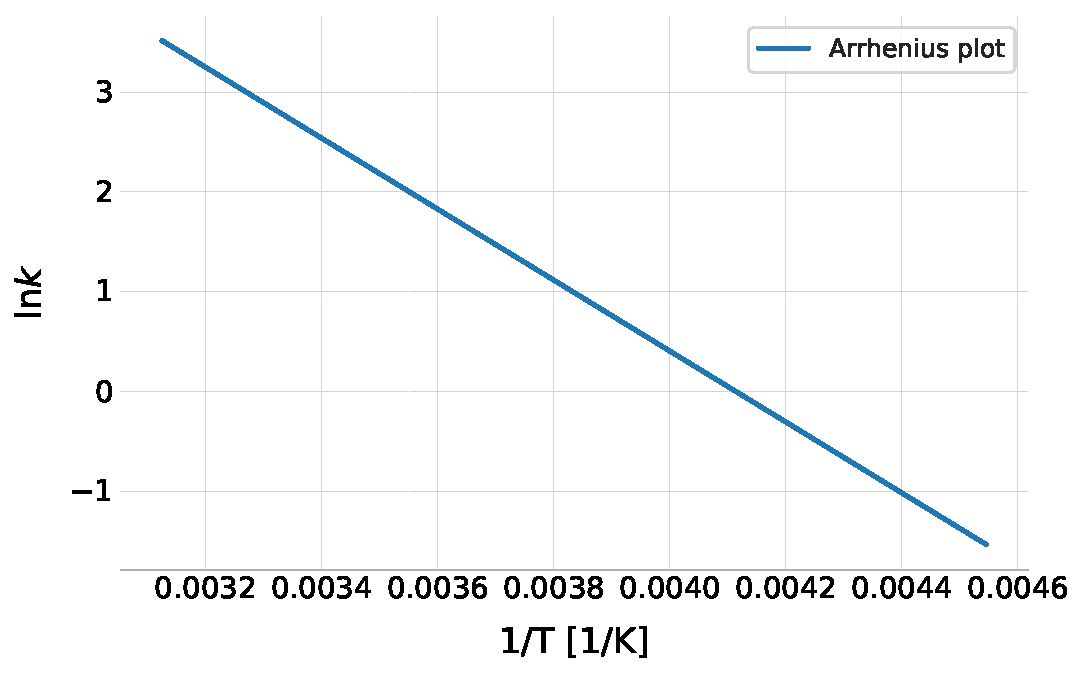
\includegraphics[width=0.4\textwidth]{figures/chemical-kinetics/arrhenius-plot}} \qquad \qquad
 		\subfloat[Extended Arrhenius plot]{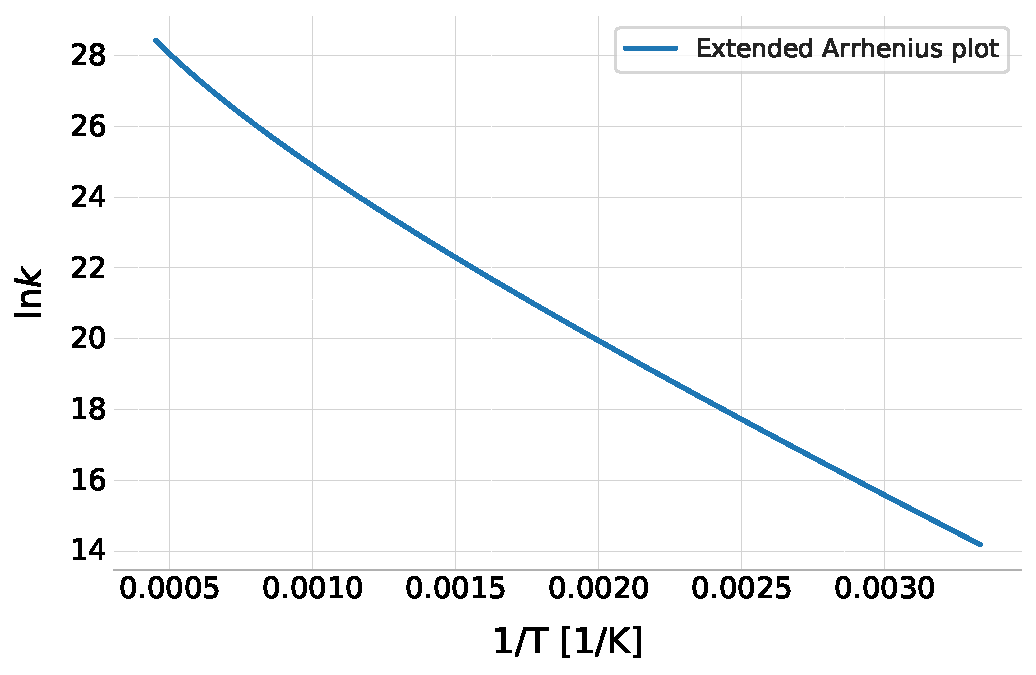
\includegraphics[width=0.38\textwidth]{figures/chemical-kinetics/extended-arrhenius-plot}}
	\end{figure}
\end{frame}
%
% --------------------------------------------------------------------------------------------------------------------%
% Pressure dependence of rate coefficients, Lindemann model
% --------------------------------------------------------------------------------------------------------------------%
%
\begin{frame}{Pressure dependence of rate coefficients, Lindemann model \, i}
	\begin{itemize}
		\item According to \alert{\bf Lindemann model}, a unimolecular decomposition is only possible if {\bf the energy in the molecule is 
		sufficient to break the bond}.
		\item Before decomposition, the energy must be added to A by means of collision with M (representation of the pressure) to obtain excited molecule A$^\star$:
		 \begin{alignat*}{2}
			\mbox{Activation} : & \quad \mathsf{A + M \xrightleftharpoons[]{k_1} A^\star + M} \\
			\mbox{Deactivation}: & \quad \mathsf{A^\star + M \xrightleftharpoons[]{k_2} A + M} \\
			\mbox{Unimolecular reaction}: & \quad \mathsf{A^\star \xrightleftharpoons[]{k_3} C}
		 \end{alignat*}
		\item The {\bf production rates} can be written as: 
		%
		 \begin{alignat*}{2}
			\tfrac{d\mathsf{[C]}}{dt}          & = k_3 \, \mathsf{[A^\star]} \\
			\tfrac{d\mathsf{[A^\star]}}{dt} & 
			= \sum_{i = 1, \ldots, 3} \nu_i r_i 
			=  r_1 - r_2 - r_3 
			= k_1 \, \mathsf{[A][M]} - k_2 \, \mathsf{[A^\star][M]} + k_3 \, \mathsf{[A^\star]}
		\end{alignat*}
	\end{itemize}
\end{frame}
%
% --------------------------------------------------------------------------------------------------------------------%
% Pressure dependence of rate coefficients, Lindemann model \, ii
% --------------------------------------------------------------------------------------------------------------------%
%
\begin{frame}{Pressure dependence of rate coefficients, Lindemann model \, ii}
	\begin{itemize}
		\item Assuming steady-state for $\mathsf{[A^\star]}$, meaning that $\tfrac{d[\mathsf{A^\star}]}{dt} = 0$, we obtain
		%
		\[
		\mathsf{[A^\star]} = \tfrac{k_1 \, \mathsf{[A]\, [M]}}{\alert<2>{k_2 \, [M]} + k_3} \qquad \mbox{and}  \qquad
		\tfrac{d\mathsf{[C]}}{dt} = \tfrac{k_1 \, k_3 \, \mathsf{[A]\, [M]}}{\alert<2>{k_2 \, [M]}  + k_3}, 
		\]
		where M represents applied pressure.\\[5pt]
	\end{itemize}
% 	\begin{itemize}
% 		%
% 		\item {\bf Under low pressure}, [M] is very small ($k_2\, \mathsf{M} \ll k_3$), then 
% 		%
% 		\[	
% 		\tfrac{d\mathsf{[C]}}{dt} = k_{\sf low} \, \mathsf{[A]\, [M]},
% 		\]
% 		%
% 		where $k_{\sf low}$ is the {\bf reaction rate coefficient at low pressure}.\\[5pt]
% 		%
% 		\pause
% 		\item {\bf For high pressure}, [M] is large  ($k_2\, \mathsf{M} \gg k_3$), then 
% 		%
% 		\[	
% 		\tfrac{d\mathsf{[C]}}{dt} = k_{\sf high} \, \mathsf{[A]},
% 		\]
% 		%
% 		where $k_{\sf high} $ is the {\bf reaction rate coefficient at high pressure}.
% 	\end{itemize}
    \vskip 20pt
	\lcol
	%\vskip 5pt
	{\bf For low pressure}: [M] is small ($k_2\, \mathsf{M} \ll k_3$), then 
	%
	\[	
	\tfrac{d\mathsf{[C]}}{dt} = k_{\sf low} \, \mathsf{[A]\, [M]},
	\]
	%
	where $k_{\sf low}$ is the {\bf reaction rate coefficient at low pressure}.
	\rcol
	{\bf For high pressure}: [M] is large  ($k_2\, \mathsf{M} \gg k_3$), then 
	%
	\[	
	\tfrac{d\mathsf{[C]}}{dt} = k_{\sf high} \, \mathsf{[A]},
	\]
	%
	where $k_{\sf high} $ is the {\bf reaction rate coefficient at high pressure}.
	\ecol
\end{frame}
%
% --------------------------------------------------------------------------------------------------------------------%
%% Reaction classification
%% --------------------------------------------------------------------------------------------------------------------%
%%
%\begin{frame}{Reaction classification}
%	\begin{itemize}
%		\item \alert{\bf Homogeneous} or \alert{\bf heterogeneous}:
%		\begin{itemize}
%			\item A {\bf homogeneous} reaction involves a single phase, e.g., 
%			%
%			\begin{alignat*}{2}
%			\mbox{Formation of ammonia}:  \mathsf{N_2(g) + 3\,H_2(g) } & \mathsf{\xrightleftharpoons[]{} 2\,NH_3(g)}\\
%			\mbox{Oxidation of sulfur dioxide}: \mathsf{2\,SO_2(g) + O_2(g) } & \mathsf{\xrightleftharpoons[]{} 2\,SO_3(g)} 
%			\end{alignat*}
%		    %
%			\item A {\bf heterogeneous} reaction involves more than one phase, e.g., 
%			\begin{alignat*}{2}
%			\mbox{Carbonatation} : \mathsf{Ca(OH)_2(s) + CO_2(g)} & \mathsf{\xrightleftharpoons[]{} CaCO_3(s) + H_2O(l)}
%	    	\end{alignat*}
%		\end{itemize}
% 	 	\item \alert{\bf Irreversible} or \alert{\bf reversible}:
%		\begin{itemize}
%			\item An {\bf irreversible} reaction is one that occurs in only one direction and continues in this direction until at least one of the reactants is depleted.
%			\item A {\bf reversible} reaction can occur in both directions (with forward and backward reaction reaction coeff. $k_f$ and $k_b$, respectively):
%			%
%			\[	
%			\mathsf{a\,A + b\,B} \xrightleftharpoons[k_f]{k_b} \mathsf{c\,C + d\,D} 
%			\quad 
%			\mbox{with equilibrium constant}
%			\quad
%			K_e := \tfrac{k_f}{k_b} = \tfrac{\mathsf{[C]^c\, [D]^d}}{\mathsf{[A]^a\,[B]^b}}.
%			\]
%			%
%		\end{itemize}
%	\end{itemize}
%\end{frame}
%
%
\begin{frame}[<+->]{Summary on reactions, their rates, rate coefficients, and orders}
	%
	\small
	\begin{itemize}
		\item The \alert{\bf overall reaction mechanism} is the result of {\bf all the elementary reactions mechanism}.
		%
		\item {\bf The reaction rate} and {\bf the reaction rate coefficient} are \alert{\bf determined by experiments}.
		%
% 		\item \alert{\bf The units of the reaction rate coefficients} $k$ depend on the relation 
% 		$[k] = \tfrac{1}{\mathsf{s \, [mol/m^3]}^{n-1}}$, where $n$ is the order of reaction. \\
		%{\bf Example}: for  the rate law $\tfrac{dw}{dt} = k \mathsf{[A][B]}$ of the second-order reaction, 
		%$[k] = \tfrac{\mathsf{m^3}}{\mathsf{s \, mol}}$. 
		%
		%
		\item {\bf The orders} are generally \alert{\bf not equal} to {\bf the stoichiometric coefficients} of the overall
		reaction equation.
		%
%		\item Unlike elementary reactions, the overall reaction rate {\bf may contain the concentration of
%		reactants, products, and catalysts}, but generally {\bf does not contain concentrations
%		of reactive intermediates}.
		%
		\item {\bf The order of reaction} is determined \alert{\bf experimentally} or by \alert{\bf means of mathematical models}.
		%
		\item The \alert{\bf most important reactions} are of: 
		\begin{itemize}
			\item zero order, 
			\item first order, and 
			\item second order.
		\end{itemize}
		%
		\item Third-order reactions {\bf are quite rare}, reactions of order greater than three are {\bf not known}.
		%	
		
	\end{itemize}
	%
\end{frame}
%
\subsection{Reaction mechanisms}
%
% --------------------------------------------------------------------------------------------------------------------%
% Reaction mechanism
% --------------------------------------------------------------------------------------------------------------------%
%
\begin{frame}{Reaction mechanisms}
	%
	\small
	\begin{itemize}
		\item The \alert{\bf kinetic mechanisms} can contain basically {\bf three types of reactions}:
		%
		\begin{itemize}
			\item in series (consecutive reactions), 
			\item in parallel (competitive reactions), and 
			\item independent.
		\end{itemize}
		%
		\pause
		\item \alert{\bf In series occurring reactions} (consecutive reactions), reactant forms an {\bf intermediate product}, which subsequently reacts to form another product:
		%
		\[\mathsf{A} \xrightleftharpoons[]{k_1} \mathsf{B} \xrightleftharpoons[]{k_2} \mathsf{C}. \]
		%
		%
		\pause
		\item \alert{\bf In parallel reactions} (competitive reactions), the reagent is consumed by two different reaction paths to form {\bf different products}:
		%
		\[\mathsf{A} \xrightleftharpoons[]{k_1} \mathsf{B} \quad \mbox{and}\quad \mathsf{A} \xrightleftharpoons[]{k_2} \mathsf{C}. \]
		%
		\pause
		\item Usually, kinetic mechanisms involve {\bf a combination of both reactions in series or parallel}.
	\end{itemize}
	%
\end{frame}
%
% --------------------------------------------------------------------------------------------------------------------%
% Example, Formation of butadiene C4H6 from ethanol
% --------------------------------------------------------------------------------------------------------------------%
%
\begin{frame}{Example, Formation of butadiene C$_4$H$_6$ from ethanol}
	%
	\begin{itemize}
		\item \alert{\bf Butadiene} $\mathsf{C_4H_6}$ is the organic compound, colorless gas that is easily condensed to a liquid.
		%
		\pause
		\item It is important industrially as a monomer in the \alert{\bf production of synthetic rubber}. 
		%
		\pause
		\item In South America, Eastern Europe, China, and India, butadiene is {\bf produced from ethanol}:		
		%
		%\item The kinetic mechanisms involve reactions in series or parallel:
		%
		%
	\end{itemize}
	\lcol
	\pause
	\begin{alignat*}{2}
		& \mathsf{C_2H_5OH \xrightleftharpoons[]{} C_2H_4 + H_2O,} \quad \mbox{(parallel)}\\
		& \mathsf{C_2H_5OH \xrightleftharpoons[]{} CH_3CHO + H_2,}  \quad \mbox{(parallel)}\\
		& \mathsf{C_2H_4 + CH3CHO \xrightleftharpoons[]{}  C_4H_6 + H_2O.}  \quad \mbox{(series)}
	\end{alignat*}
	\rcol
	\begin{figure}[!t]
		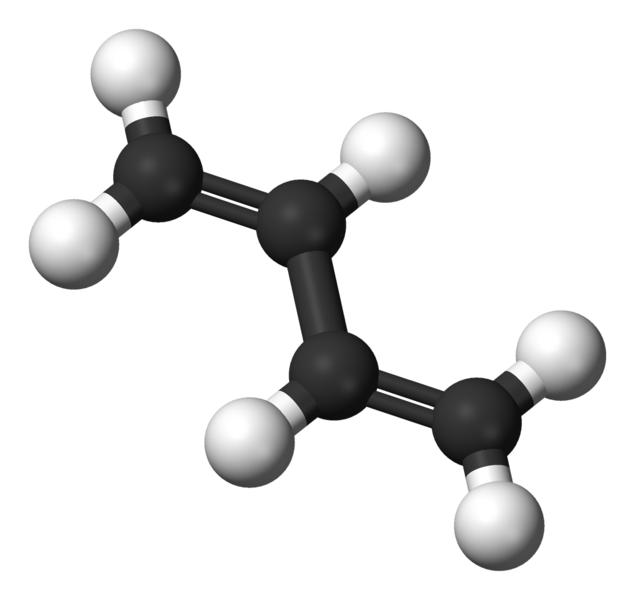
\includegraphics[scale=0.15]{figures/chemical-kinetics/butadiene.png}
		\caption{Organic compound of $\mathsf{(CH2=CH)_2}$.}
	\end{figure}
	\ecol
	%
\end{frame}
%
% --------------------------------------------------------------------------------------------------------------------%
% Chain reactions, Ignition of hydrogen
% --------------------------------------------------------------------------------------------------------------------%
%
\begin{frame}[<+->]{Chain reactions, Ignition of hydrogen example}
	\small
	%
	\begin{itemize}
		\item \alert{\bf Chain reactions} (type of the consecutive reactions) are defined by reactives intermediate reacting to produce another intermediates, 
		have complex kinetics, and occur quickly.
		%
		\item The intermediate species in a chain reaction is \alert{\bf a chain propagator}:
		%
		\begin{multline*}
			\mbox{reactant} \xrightarrow[]{\text{initiation}} \mbox{propagator 1} \xrightarrow[]{\text{chain branch i}} \ldots
			\xrightarrow[]{\text{chain branch i}} \mbox{propagator i} \xrightarrow[]{\text{termination}} \mbox{products} 
		\end{multline*}
		%
		\item They are the basis of \alert{\bf combustion processes}, rapid reactions of species with O$_2$ generating heat. 
		%
	\end{itemize}
	\begin{table}
		\begin{tabular*}{1\textwidth}{@{\extracolsep{\fill}}lll}
			\toprule 
			N & Reaction & Step \\[-5pt]
			\midrule 
			1 & $\mathsf{H_2 + O_2 \xrightleftharpoons[]{} 2\, OH^\star}$ &	initiation of the step \\[-3pt]
			2 & $\mathsf{OH^\star + H_2 \xrightleftharpoons[]{} H_2O + H^\star}$ &	propagation of the chain \\[-3pt]
			3 & $\mathsf{H^\star + O_2 \xrightleftharpoons[]{} OH^\star + O^\star}$ & branch of the chain \\[-3pt]
			4 & $\mathsf{O^\star + H_2 \xrightleftharpoons[]{} OH^\star + H^\star}$ & branch of the chain  \\[-3pt]
			5 & $\mathsf{H^\star \xrightleftharpoons[]{} 0.5 \, H_2}$ &	termination of the chain \\[-3pt]
			6 & $\mathsf{H^\star + O_2 + M \xrightleftharpoons[]{} HO_2^\star +M^\star }$ & propagation of the chain \\[-3pt]
			\bottomrule
		\end{tabular*}
		%
		\caption{Important reactions for the hydrogen ignition mechanism.}
	\end{table}
	%
\end{frame}
%
\subsection{Redox reaction}
%	
% --------------------------------------------------------------------------------------------------------------------%
% Redox reaction
% --------------------------------------------------------------------------------------------------------------------%
%
\begin{frame}{Redox reaction}
	\small
	\begin{itemize}
		\item \alert{\textbf{Redox (or reduction-oxidation) reaction}} is a type of chemical reaction that involves a transfer 
		of electrons between two species.
		\pause
		\item { \bf Examples}: 
		\begin{itemize}
				\item body uses redox reactions to convert food and oxygen to energy plus water and CO2;
				\item batteries in electronics rely on redox reactions;
				\item combustion reactions in the car engines, e.g., combustion of octane (hydrocarbon)
				%
				\[
				\mathsf{2 \, C_8\, H_{18} + 25\,O_2 \rightarrow 16\, CO_2(g) + 18\,H_2O}.
				\]			
		\end{itemize}
		%
		\pause
		\item The $\mathsf{H_2O}$ can be 
		%
		\begin{itemize}
			%\item ionized
			%%
			%\[
			%\mathsf{H_2O(l) = H^+ + OH^-,}
			%\]
			%
			\item (or oxygen in it) \alert{\bf oxidized}, losing electron, 
			%
			$\mathsf{H_2O(l) = O_2(aq) + 2\, e^{-} + 2\, H^+,}$ or 
			
			%
			\item (or hydrogen in it) \alert{\bf reduced}, accepting electron, 
			%
			%\[
			$
			\mathsf{H_2O(l) + e^{-} = \tfrac{1}{2} \, H_2(aq) + OH^-.}$
			%\]
			%
		\end{itemize}
		%
		\pause
		\item \alert{\bf Self-redox} is the reaction, where the same element undergoes oxidation and reduction simultaneously,  
		\[
		\mathsf{2\, NaOH + Cl_2 \rightarrow NaCl + NaClO + H_2O,}
		\]
		%
		where Cl$^0$ with oxidation number 0, becomes Cl$^{-1}$  in NaCl and Cl$^{+1}$  in NaClO. 
	\end{itemize}
\end{frame}
%
% --------------------------------------------------------------------------------------------------------------------%
% Oxidation number, Oxidizers and reducers 
% --------------------------------------------------------------------------------------------------------------------%
%
\begin{frame}{Oxidation number, Oxidizers and reducers }
	\small
	\begin{itemize}
		\item \alert{\textbf{Oxidation number}} (NOX) of a chemical element is  the number of charges that an atom would 
		possess if the electrons were not shared but located entirely on a single atom.
	\end{itemize}
	%
	\pause 
	\vskip -25pt
	\begin{columns}
		\begin{column}{0.6\textwidth}
			\begin{itemize}
				\item {\bf Examples}: 
				\begin{itemize}
					\item water H$_2$O: H$^+$ -- O$^{-2}$ -- H$^+$ ;
					\item sulfuric acid H$_2$SO$_4$: with H$^+$,  S$^{6+}$, and O$^{-2}$.
				\end{itemize}
			\end{itemize}
		\end{column}
		\begin{column}{0.3\textwidth} 
			\begin{figure}[!t]
				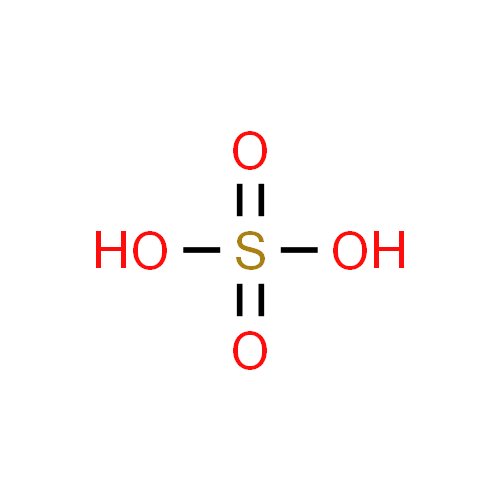
\includegraphics[width=0.8\columnwidth]{figures/chemical-kinetics/sulfuric-acid.png}
			\end{figure}
		\end{column}
	\end{columns}
	%
	\vskip -15pt
	\pause
	\begin{itemize}
	\item \alert{\bf Oxidizer} causes the oxidation and receives electron:
	\begin{itemize}
		\item halogens, such as F$_2$ and Cl$_2$;
		\item oxyacid and oxyanions, such as NO$^-_3$, IO$^-_3$, and MnO$^-_4$;
		\item forms of oxygen, such as O$_3$; and
		\item peroxides, such as H$_2$O$_2$.
	\end{itemize}
 	\pause
	\item \alert{\bf Reducer} causes the reduction and gives away electron:
	\begin{itemize}
		\item alkali and alkaline earth metals, Li and Na.
	\end{itemize}
	\end{itemize}
\end{frame}
%
% --------------------------------------------------------------------------------------------------------------------%
% Basic rules of the redox number determination
% --------------------------------------------------------------------------------------------------------------------%
%
\begin{frame}{Basic rules of the redox number determination}
	\vskip 10pt
	\begin{figure}[!t]
		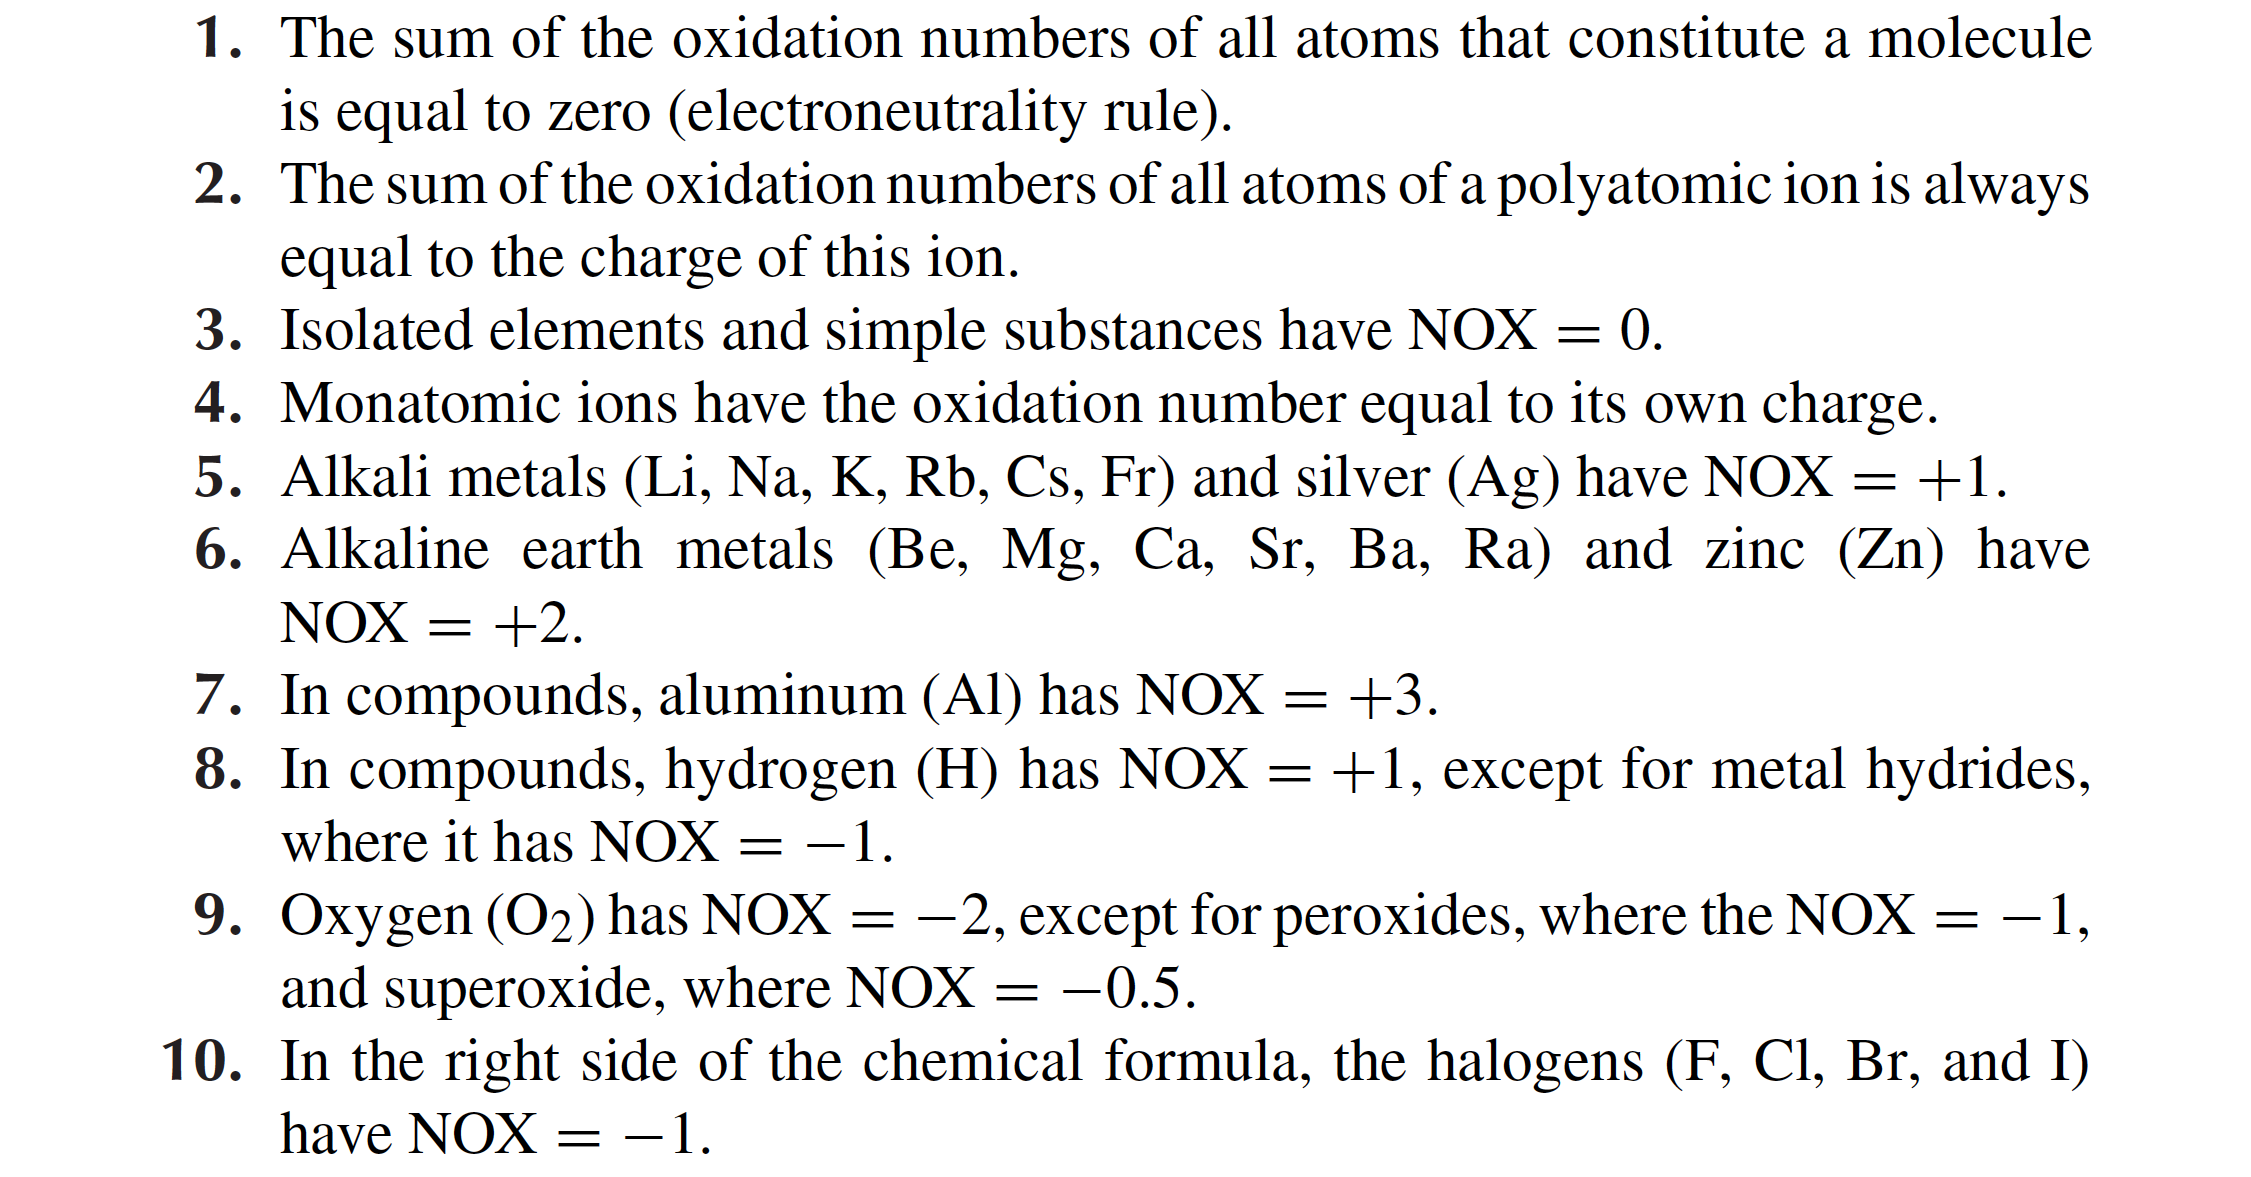
\includegraphics[width=0.77\columnwidth]{figures/chemical-kinetics/nox-rules.png}
		\caption{From \emph{Modeling and Simulation of Reactive Flows} by Bortoli, Andreis, and Pereira, 2015.}
	\end{figure}
\end{frame}
%
% --------------------------------------------------------------------------------------------------------------------%
% Concepts of half-reaction
% --------------------------------------------------------------------------------------------------------------------%
%
\begin{frame}{Concepts of half-reaction}
	\begin{itemize}
		\item The redox reactions can be expressed as a combination of two partial ionic reactions:
		\begin{itemize}
			\item an \alert{\bf oxidation half-reaction}
			\[
			\mathsf{Red_1 \rightarrow Ox_1 + \nu_1 e^-.}
			\]
			\item and a \alert{\bf reduction half-reaction}
				\[
			\mathsf{Ox_2 + \nu_2 e^- \rightarrow Red_2.}
			\]
		\end{itemize}
		\item \alert{\bf Example}: reaction $\mathsf{2\, H_2 + O_2 \rightarrow 2\, H_2O}$ can be decoupled to
		\begin{itemize}
			\item an \alert{\bf oxidation half-reaction} (of hydrogen) \qquad $\mathsf{H_2 \rightarrow 2\, H^+ + 2 e^-}$ and
			%
			\item a \alert{\bf reduction half-reaction} (of oxygen) \qquad $\mathsf{O_2 + 4\, e^- + 2 H^+ \rightarrow 2\, OH^-.}$
			%
			\item In a linear combination of these equations, 
			{\bf the number of donated electrons} must be {\bf equal} to {\bf the number of received electrons}:
			%
			$$
			\begin{array}{l}
				+
				\begin{cases}
					\mathsf{2 \, H_{2}} & \rightarrow\mathsf{4 \, H^{+}+4 \, e^{-}}\\
					\mathsf{O_{2}+4 \, e^{-}+2 \, H^{+}} & \rightarrow\mathsf{2 \, OH^{-}}
				\end{cases}\\
				\hline \qquad\qquad\qquad\mathsf{2  \,  H_{2}+O_{2} \rightarrow 2 \, H^{+}+2 \, OH^{-} = 2 \, H_{2}O}
			\end{array} 
			$$
		\end{itemize}
	\end{itemize}

\end{frame}
%
% --------------------------------------------------------------------------------------------------------------------%
% Balancing redox reaction, Example
% --------------------------------------------------------------------------------------------------------------------%
%
%Al(s)+2H+(aq)→Al3+(aq)+H2(g)
%
%
%1. Al(s)→Al3+(aq) +3e- x 2
%2. 2H+(aq) +2e-→H2(g) x 3
%----------
%
%2Al(s) + 6H+(aq) → 2Al3+(aq) + 3H2(g)
%\begin{frame}{Balancing redox reaction, Example}
%	
%	\begin{itemize}
%		\item Atoms appear to be balanced, but \alert{charges are not}:\\[-5pt]
%		
%		\[
%		\mbox{\alert{charge 2+}}
%		\qquad
%		\mathsf{Al(s)+2\, H^{+}(aq) \rightarrow Al^{3+}(aq)+H_2(g).}
%		\qquad
%		\mbox{\alert{charge 3+}}
%		\]
%		
%		\item Reduction half-reaction ($\mathsf{H^{+}}$ is being reduced to $\mathsf{H_2(g)}$):\\[-5pt]
%		
%		\[
%		\mbox{\alert{charge 0}}
%		\qquad
%		\mathsf{H^{+}(aq) +  2\, e^{-} \rightarrow H_2(g).}
%		\qquad
%		\mbox{\alert{charge 0}}
%		\]
%		
%		\item Oxidation half-reaction ($\mathsf{Al(s)}$ is being oxidized to $\mathsf{Al^{3+}(aq)}$):\\[-5pt]
%		
%		\[
%		\mbox{\alert{charge 0}}
%		\qquad
%		\mathsf{Al(s) \rightarrow Al^{3+}(aq) +  3\, e^{-} .}
%		\qquad
%		\mbox{\alert{charge 0}}
%		\]
%		
%		\item Linear combination to obtain \alert{\bf charge-balanced reaction}: 
%		
%		$$
%		\begin{array}{c}
%			+\begin{cases}
%				\mathsf{6\,H^{+}(aq)+6\:e^{-}} & \rightarrow\mathsf{3\,H_2(g)}\\
%				\mathsf{2\,Al(s)} & \rightarrow\mathsf{2\,Al^{3+}(aq)+6\:e^{-}}
%			\end{cases}\\[5pt]
%			\hline \qquad\mathsf{\;6\,H^{+}(aq)+2\,Al(s)\rightarrow2\,Al^{3+}(aq)+}\mathsf{3\,H_2(g)}.
%		\end{array}
%	    $$
%		\end{itemize}
%	
%\end{frame}
%%
%% --------------------------------------------------------------------------------------------------------------------%
%% Solubility in redox reactions
%% --------------------------------------------------------------------------------------------------------------------%
%%
%\begin{frame}{Solubility in redox reactions}
%	\begin{itemize}
%		\item For a solid that dissolves in a redox reaction, \textbf{solubility} is expected to \alert{\textbf{depend on the potential}}.
%		\item Example: 
%		%For example, solubility of
%		%gold in high-temperature water is observed to be almost an order of magnitude higher (i.e. about ten times
%		%higher) when the redox potential is controlled using a highly oxidizing Fe3O4-Fe2O3 redox buffer than with a
%		%moderately oxidizing Ni-NiO buffer.
%		
%	\end{itemize}
%	
%\end{frame}
%
%
\begin{frame}{Quiz on redox reaction}
	\begin{itemize}
		\item \alert{\textbf{Quiz}}: determine what is the oxidizing and reducing agents in the following reaction?
		%
		\[
		\mathsf{Zn + 2\, H^+ \rightarrow  Zn^{2+} + H_2}.
		\]
		%
		Reminder: 
			\begin{itemize}
				\item \textbf{reducing agent} is the one that \textbf{forces other species to gain electron}, and 
				\item \textbf{oxidizing agent}  is the one that \textbf{forces other species to lose one}):
			\end{itemize}
		
		\begin{center}
			\href{http://etc.ch/wsKw}{\textcolor{indigo(dye)}{\tt http://etc.ch/wsKw}} \quad or \quad
			
\includegraphics[height=0.15\columnwidth]{figures/chemical-kinetics/polls.png}
		\end{center}
		\hiddenpause
		\item {\textbf{Answer}}: The oxidation state of H changes from +1 to 0, and the oxidation state of  Zn  changes from 0 to +2. \\
		Hence,  Zn  is oxidized and acts as the reducing agent.  $\mathsf{H^+}$  ion is reduced and acts as the oxidizing agent.
		
	\end{itemize}
	
\end{frame}

\begin{frame}{Combustion reactions}

	\begin{itemize}
	\item \alert{\textbf{Combustion }} is the formal terms for `burning' and typically involves a \textbf{substance reacts with oxygen to transfer energy to the surroundings} as light and heat. \\
	 %Hence, combustion reactions are almost always exothermic. 
	 \item {\textbf{Example}}: internal combustion engines rely on the combustion of organic hydrocarbons  $\mathsf{C_xH_y}$  to generate  $\mathsf{CO_2}$  and   $\mathsf{H_2O}$:
	%
	\[
	\mathsf{C_xH_y + O_2 \rightarrow CO_2 + H_2O.}
	\]
	\vskip -10pt
	%
	\pause
	\item Many chemicals can `burn' in \textbf{other environments}. \\
	%
	{\textbf{Example 1}}: metals like  titanium and magnesium can burn in nitrogen:
	%
	\begin{alignat*}{2}
		& \mathsf{2\,Ti(s)+N_2(g) \rightarrow 2\, TiN(s),} \\
		& \mathsf{3\,Mg(s)+N_2(g) \rightarrow Mg_3N_2(s).} 
	\end{alignat*}
	%
	{\textbf{Example 2}}: chemicals can be also oxidized by other chemicals than oxygen, such as $\mathsf{Cl_2}$ or $\mathsf{F_2}$; these processes are also considered combustion reactions.
	\end{itemize}
	%
\end{frame}
%
\begin{frame}{Quiz on redox reaction}
	\begin{itemize}
		\item \alert{\textbf{Quiz}}:  which of the following are combustion reactions?\\[-20pt]
		%
		\begin{alignat*}{2}
			& \mathsf{(a) \quad 2\,H_2O \rightarrow 2\,H_2+O_2,} \\[-3pt]
			& \mathsf{(b) \quad 4\,Fe+3\,O_2 \rightarrow 2\,Fe_2O_3, }\\[-3pt]
			& \mathsf{(c) \quad  2\,AgNO_3+H_2S \rightarrow Ag_2S+2\,NHO_3, }\\[-3pt]
			& \mathsf{(d) \quad  2\,Al+N_2 \rightarrow 2\,AlN_4.}
		\end{alignat*}
		%
    	 \vskip -40pt
		\begin{center}
			\href{http://etc.ch/wsKw}{\textcolor{indigo(dye)}{\tt http://etc.ch/wsKw}} \quad or \quad
			
\includegraphics[height=0.17\columnwidth]{figures/chemical-kinetics/polls.png}
		\end{center}
		\hiddenpause
		\item {\textbf{Answer}}: Reactions (b) and (d) are combustion reactions with different oxidizing agents. \\
		Reaction  (b) is the conventional combustion reaction using  $\mathsf{O_2}$  and (d) uses  $\mathsf{N_2}$  instead.
		
	\end{itemize}
	
\end{frame}
%--------------------------------------------------------------------------------------------------------------------%
% Basic Simplification Principles in Reaction Kinetics
% --------------------------------------------------------------------------------------------------------------------%
\subsection{Simplification principles in reaction kinetics}
%
\begin{frame}{Simplification/reduction principles in reaction kinetics}
	%
	\begin{itemize}
		\item  If applied appropriately, the following \alert{\bf kinetic simplification/reduction principles} may provide a nearly identical
		solution compared to the original system of ODEs:
		%
		\begin{itemize}
			\item the pool chemical / pool component  approximation, 
			\item the pre-equilibrium approximation, 
			\item the rate-determining step, and 
			\item  the quasi-steady-state approximation.
		\end{itemize}
		%		
		\pause
		\item Reduction principles \alert{\bf only valid under certain conditions}, e.g., the results are reliable for certain temperature ranges.
	\end{itemize}
	%
\end{frame}
%
% --------------------------------------------------------------------------------------------------------------------%
% Pool chemical approximation
% --------------------------------------------------------------------------------------------------------------------%
%
\begin{frame}{Pool chemical / pool component approximation}
	%
	\small
	\begin{itemize}
		\item \alert{\bf Pool chemical / pool component approximation} applicable when 
		\begin{itemize}
			\item the concentration of a reactant species is {\bf much higher} than those of the other species, and, therefore, 
			\item the concentration change of this species is {\bf considered to be negligible} throughout the simulation period.
		\end{itemize}
	    \pause
		\item \alert{\bf Example}: a {\bf second-order reaction} step $\mathsf{A+ B \rightarrow C}$ can be converted to {\bf first-order} $\mathsf{A \rightarrow C}$,
		assuming $\mathsf{[B]} \approx {\rm const}$ during the simulations.
		%
		\begin{itemize}
			\item We introduce a new rate coefficient
			%
			\[k\prime := k \, \mathsf{[B]} \approx {\rm const}.\]
			\vskip -10pt
			%
			\item Then, the second-order expression can be converted to a first-order one: 
			%
			\[
			\tfrac{d\mathsf{[C]}}{dt} = k \, \mathsf{[A]\,[B]} = k^\prime \, \mathsf{[A]}.
			\]
			\vskip -10pt
		\end{itemize}
		%		
		\pause
		\item This particular case is called a  \alert{\bf pseudo-first-order approximation} and 
		$k^\prime$ is the \alert{\bf pseudo-first-order rate coefficient.}
	\end{itemize}
	%
\end{frame}
%
% --------------------------------------------------------------------------------------------------------------------%
% Pre-equilibrium approximation
% --------------------------------------------------------------------------------------------------------------------%
%
\begin{frame}{Pre-equilibrium / partial equilibrium / fast equilibrium approximation \,i}
	%
	\small
	\begin{itemize}
		\item \alert{\bf Partial equilibrium / fast equilibrium approximation} applicable when the {\bf species participating 
		in a pair of fast-equilibrium reactions are consumed by slow reactions.}
		%
			\begin{itemize}
			\item[(i)] In case {\bf of equilibrium}, the rates of the forward and backward reactions are equal $\Rightarrow$ 
			the concentrations of the participating species can be calculated from the stoichiometry and the equilibrium constant.\\
			%
			{\bf Example}: consider equilibrium reaction $\mathsf{A \xrightleftharpoons[k_2]{k_1} B}$ with equilibrium $K_e := \tfrac{k_1}{k_2}$ \\
			%
			$\Rightarrow$ in case of {\bf equilibrium}: $k_1 \, \mathsf{[A]} = k_2 \, \mathsf{[B]}$.
			%
			\item \alert{\bf Quiz}: how can we express concentrations of B?
			%
			\begin{center}
				\href{http://etc.ch/wsKw}{\textcolor{indigo(dye)}{\tt http://etc.ch/wsKw}} \quad or \quad 
				
\includegraphics[height=0.18\columnwidth]{figures/chemical-kinetics/polls.png}
			\end{center}
			\vskip 10pt
			\hiddenpause
			\item  {\bf Answer}: $\mathsf{[B]} = K_e \, \mathsf{[A]}$.
			\end{itemize}	
%		\item {\bf Example I }: consider equilibrium reaction $\mathsf{A \xrightleftharpoons[k_2]{k_1} B}$ with equilibrium $K_e := \tfrac{k_1}{k_2}$: \\
%		%
%		$\Rightarrow$ in case of {\bf an onset of equilibrium}: $k_1 \, \mathsf{[A]} = k_2 \, \mathsf{[B]}$, therefore $\mathsf{[B]} = K_e \, \mathsf{[A]}$\\[10pt]
					%	
	%
	\end{itemize}
	%
\end{frame}
\begin{frame}{Pre-equilibrium / partial equilibrium / fast equilibrium approximation \,ii}
	%
	\small
	\begin{itemize}
	   	\item[(ii)] If the {\bf  rates of the equilibrium reactions are much higher than the rates of the other reactions consuming 
				these species} $\Rightarrow$  concentrations of these species are determined by the equilibrium reactions only.\\
			%
			{\bf Example}: consider equilibrium reaction $\mathsf{A \xrightleftharpoons[k_2]{k_1} B \xrightarrow{k_3} C}$, where $k_3 \ll k_1, k_2$ \\
			%
% 			$\Rightarrow$ assuming $\mathsf{[B]} = K_e \, \mathsf{[A]}$, therefore $\tfrac{d\mathsf{[C]}}{dt} = k_3 \, \mathsf{[B]}$.		\\[10pt]
		%
		\item \alert{\bf Quiz}: assuming $\mathsf{[B]} = K_e \, \mathsf{[A]}$, how can we express the production rate of C?		
		%
		\begin{center}
			\href{http://etc.ch/wsKw}{\textcolor{indigo(dye)}{\tt http://etc.ch/wsKw}} \quad or \quad 
			
\includegraphics[height=0.18\columnwidth]{figures/chemical-kinetics/polls.png}
		\end{center}
		\hiddenpause
		\vskip 10pt
		\item  {\bf Answer}: $\tfrac{d\mathsf{[C]}}{dt} = k_3 \, \mathsf{[B]} = k_3\, K_e \, \mathsf{[A]}$.	
		\end{itemize}	
		%		\item {\bf Example I }: consider equilibrium reaction $\mathsf{A \xrightleftharpoons[k_2]{k_1} B}$ with equilibrium $K_e := \tfrac{k_1}{k_2}$: \\
		%		%
		%		$\Rightarrow$ in case of {\bf an onset of equilibrium}: $k_1 \, \mathsf{[A]} = k_2 \, \mathsf{[B]}$, therefore $\mathsf{[B]} = K_e \, \mathsf{[A]}$\\[10pt]
		%	
		%
	%
\end{frame}
%
%
% --------------------------------------------------------------------------------------------------------------------%
% Example, Complex souring system
% --------------------------------------------------------------------------------------------------------------------%
%

\begin{frame}{Example, Complex souring system}
	%
	\small 
	\begin{itemize}
		\item Kinetics modeling  of souring of complex system for approx. 58.33 days with minerals: \\[5pt]
		\lcol
		\hspace*{2cm}
		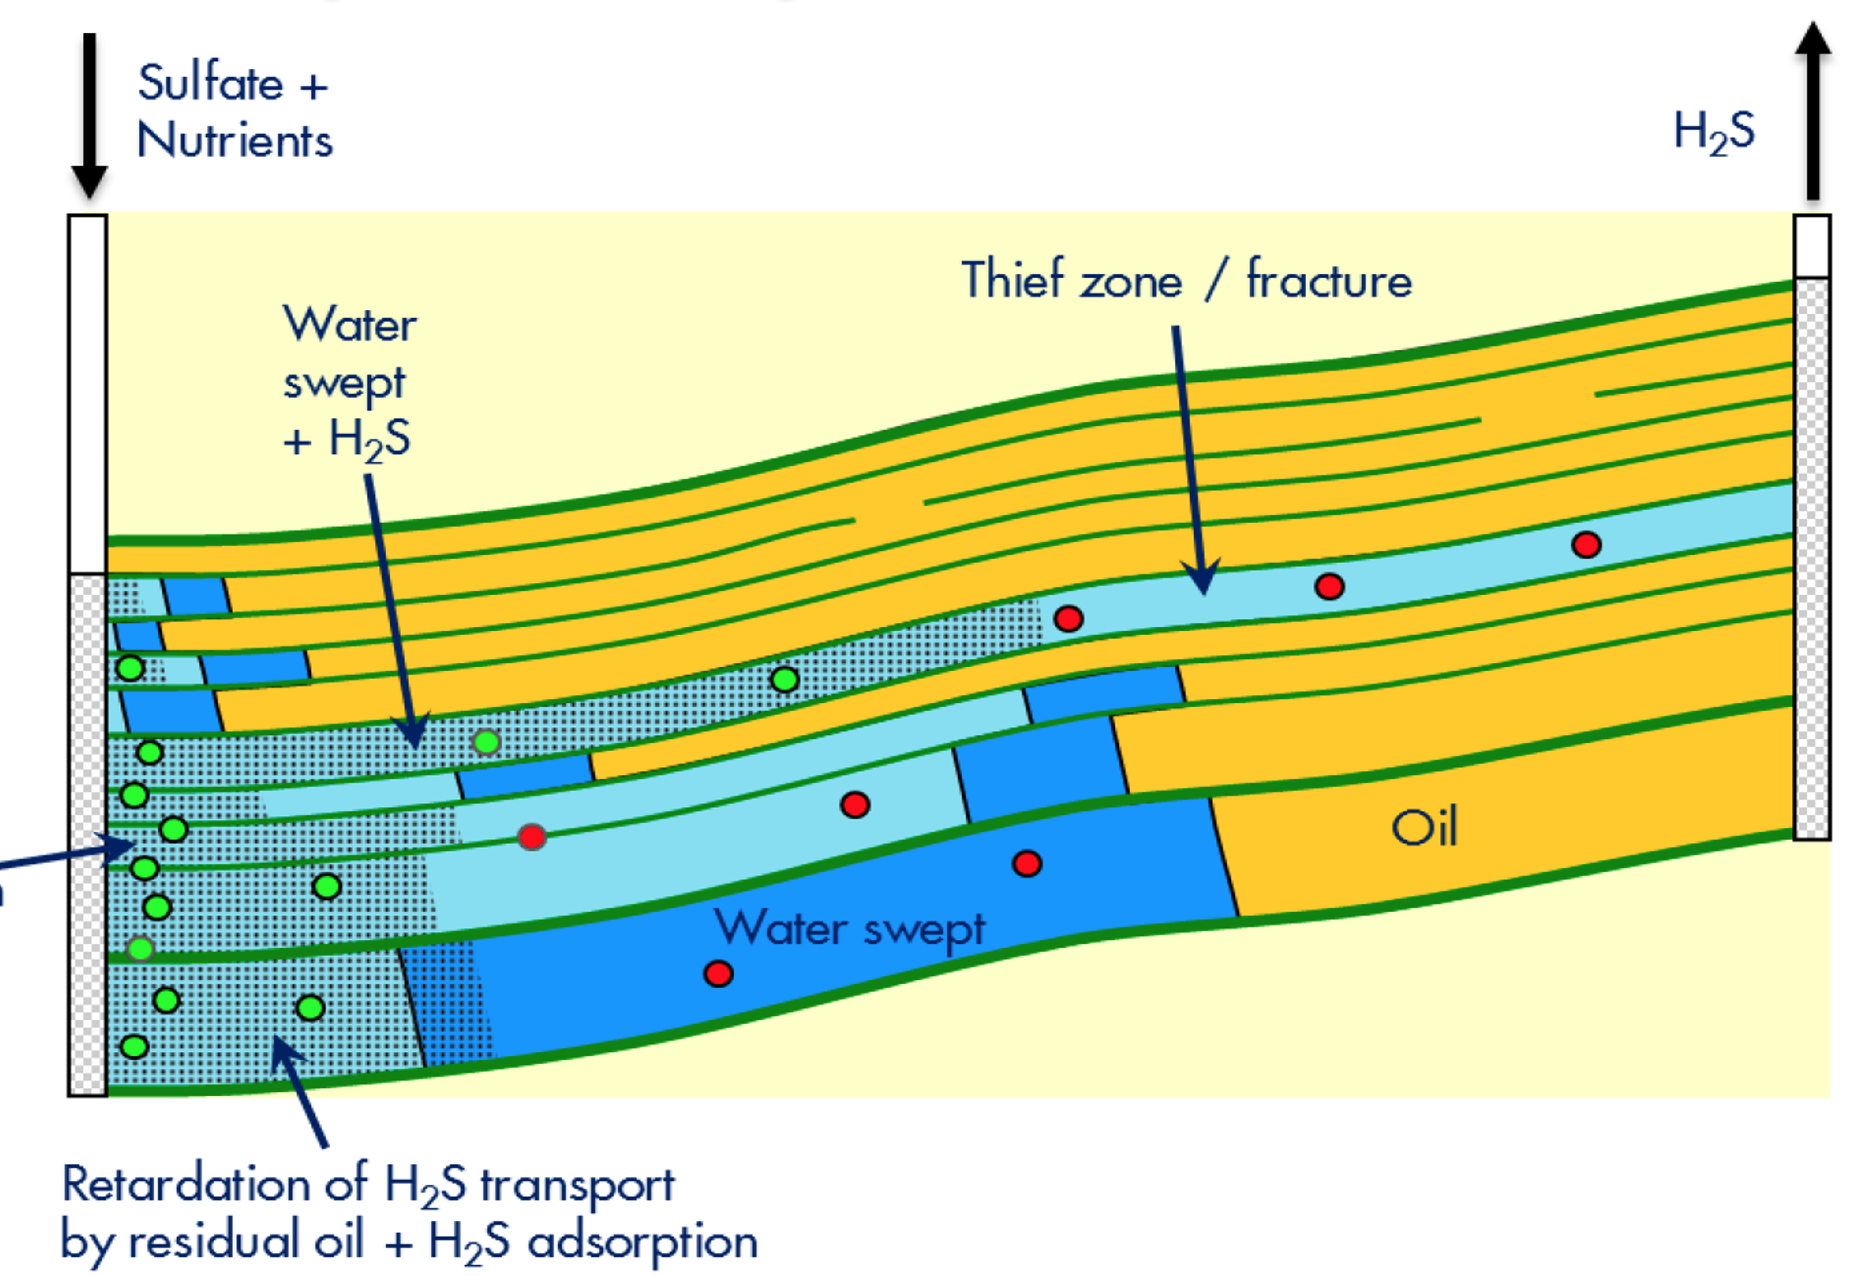
\includegraphics[width=0.6\textwidth]{figures/chemical-kinetics/souring.png}
		\rcol
		{\scriptsize
			\vskip -15pt
			\begin{itemize}
				\item Calcite,      $k_{\mathsf{Calcite}} \sim 10^{-1}$,  \\[-15pt]
				\item Daphnite,      $k_{\mathsf{Daphnite}} \sim 10^{-9}$,\\[-15pt]
				\item Kaolinite,     $k_{\mathsf{Kaolinite}} \sim 10^{-11}$,  \\[-15pt]
				\item Siderite,  $k_{\mathsf{Siderite}}  \sim 10^{-6}$,\\[-15pt]
				\item Quartz, $k_{\mathsf{Quartz}} ~10^{-10}$
			\end{itemize}
		}
		\ecol
	\vskip 5pt	
	%
	\item Assuming that calcite is controlled by equilibrium, we obtained the speedup of $\approx$ \alert{\bf 4.24x}. 
	\end{itemize}
	\vskip -15pt
	\begin{figure}[!t]
		\centering
		\subfloat[Calcite, daphnite, and kaolinite ]{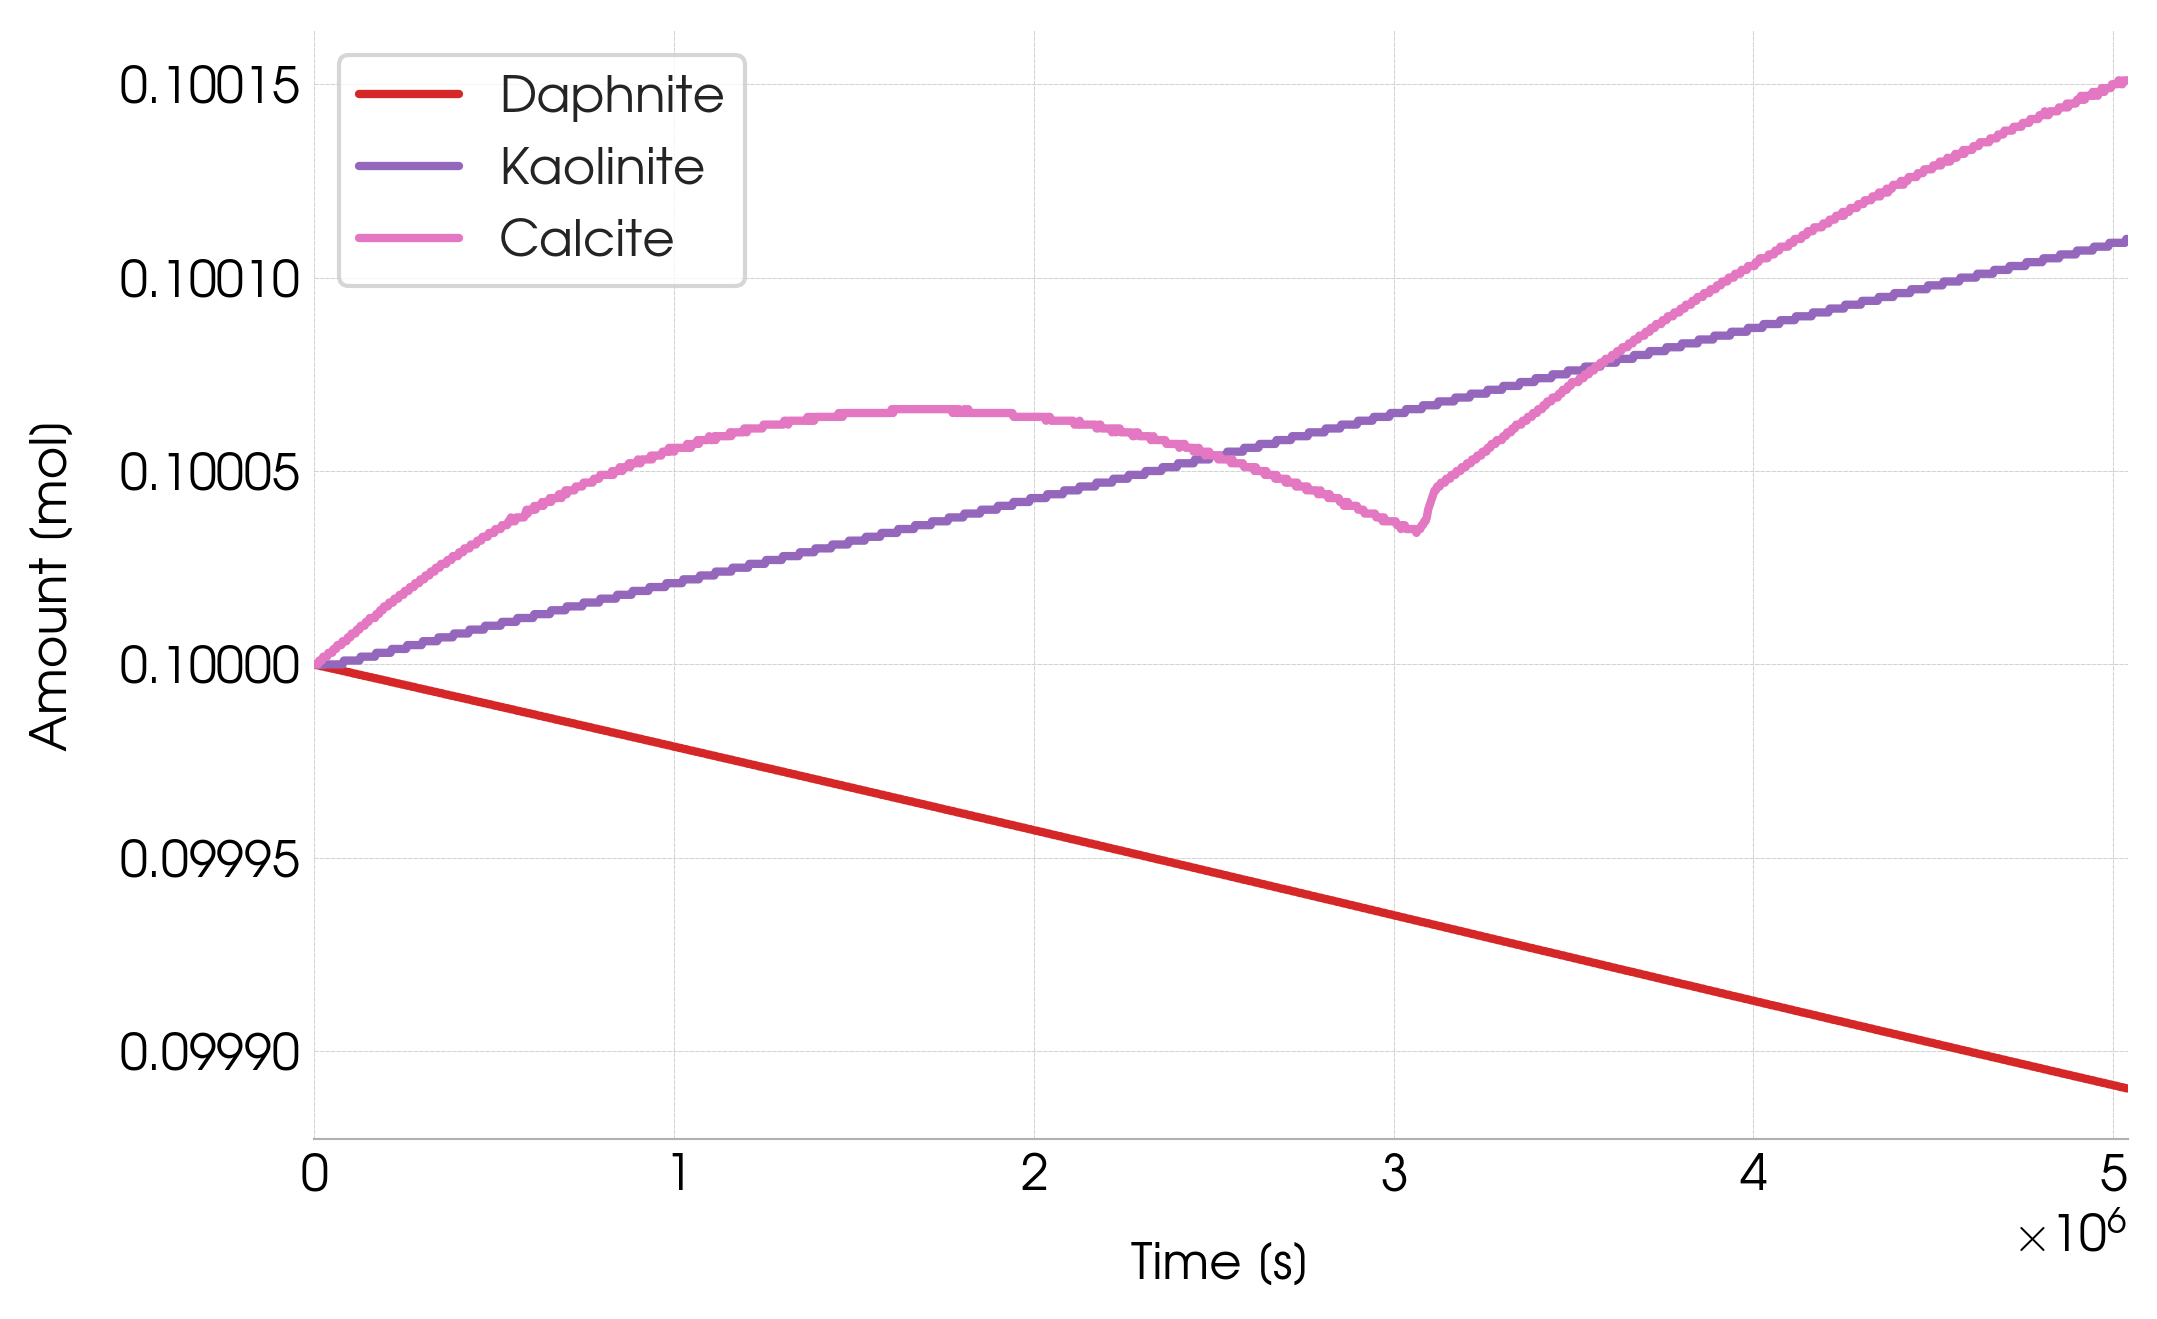
\includegraphics[width=0.35\textwidth]{figures/chemical-kinetics/reaktoro-daphnite-kaolinite-calcite.png}} \qquad \qquad
		\subfloat[Pyrrhotite and siderite over time]{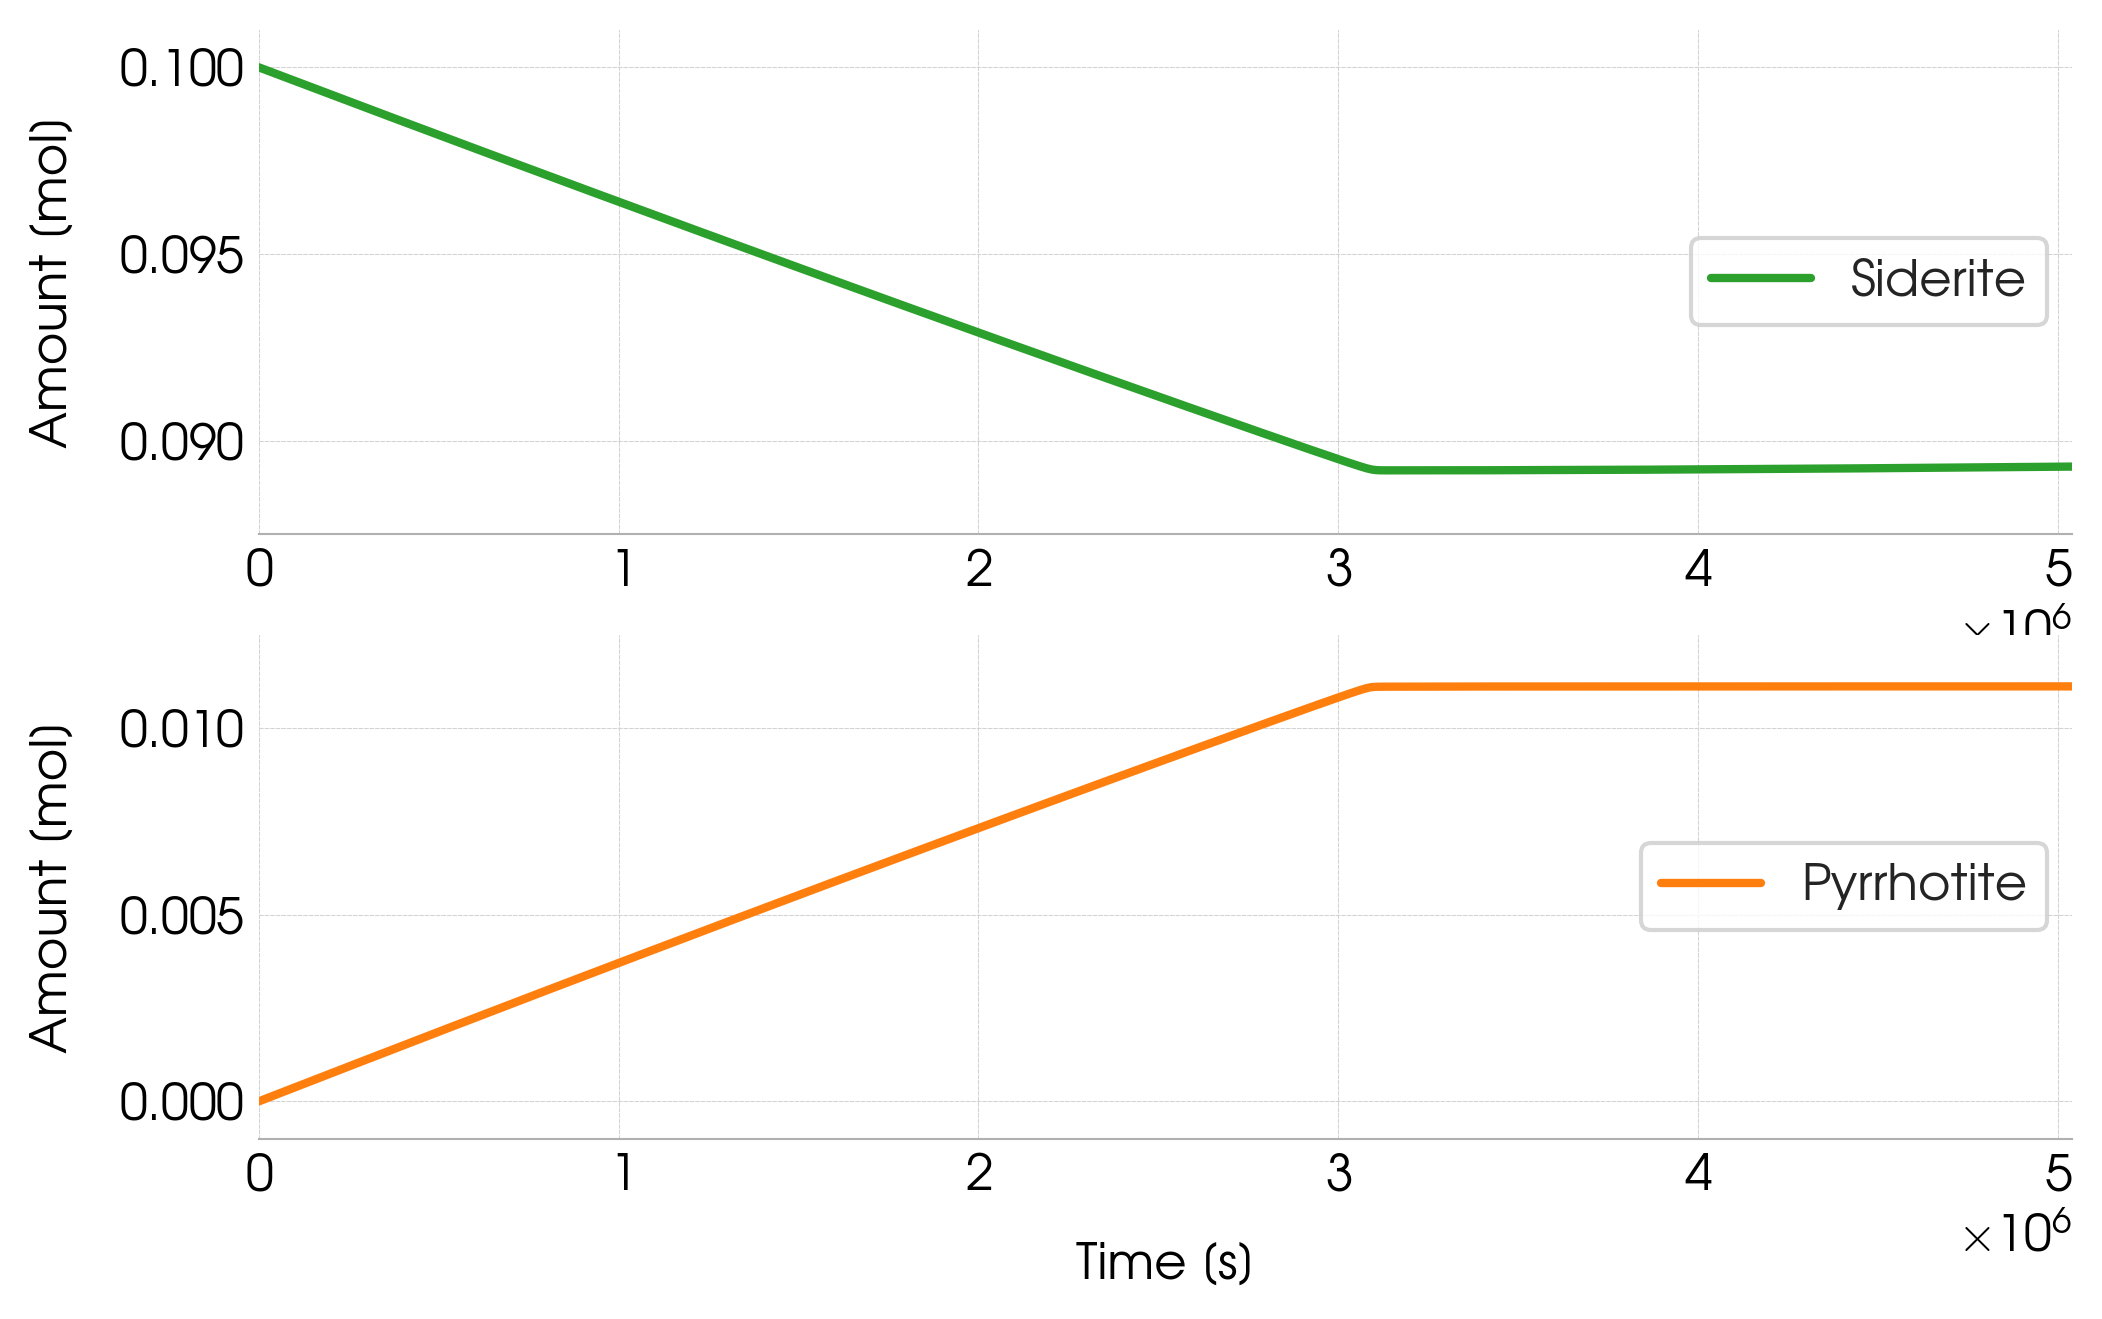
\includegraphics[width=0.33\textwidth]{figures/chemical-kinetics/reaktoro-pyrrhotite-siderite.png}}
	\end{figure}
\end{frame}

%
% --------------------------------------------------------------------------------------------------------------------%
% Rate-determining step
% --------------------------------------------------------------------------------------------------------------------%
%
\begin{frame}{Rate-determining step}
	% 
	\begin{itemize}
		%\item \alert{\bf Rate-determining step} is rate coefficient of a single reaction step that could determine 
		 %the production rate of a reactant or final product of the overall chemical reaction. 
		%		
		%\pause
		\item For {\bf sequential first-order reactions}, the reaction step having \alert{\bf the smallest rate coefficient is the rate-determining one}.
		\pause
		%
		\item {\bf Example}: in the reaction 
		$\mathsf{A \xrightarrow[]{k_1} B \xrightarrow[]{\boldsymbol{\alert{k_2}}} C \xrightarrow[]{k_3} D \xrightarrow[]{k_4} E \xrightarrow[]{k_5} P}$ and 
		$k_2 \ll k_1, k_3, k_4, k_5$, then 
		%
		\[\tfrac{d\mathsf{[P]}}{dt} = k_2 \, \mathsf{[B]}.\]
%		\vskip -10pt
%		\pause
%		\item In the {\bf general case}, one investigates sensitivity of the production rate $\tfrac{d\mathsf{[A_i]}}{dt}$ with respect to 
%		a small change of rate coefficient $k_i$, which available from the Jacobian (sensitivity matrix)
%		%
%		\[J := \Big\{ J_{ij} \Big\}_{i, j = 1, ..., \mathsf{N}} = \Big\{ \partial \tfrac{d\mathsf{[A_i]}}{dt} / \partial k_j \Big\}_{i, j = 1, ..., \mathsf{N}}.\]
%		\vskip -10pt
%		%
%		\pause
%		\item If $J_{ij}$ is much higher for reaction $j$ than for the other reaction steps,
%	    then reaction $j$ is {\bf the rate determining step of the production of species $i$}.
	\end{itemize}
	%
\end{frame}
%
% --------------------------------------------------------------------------------------------------------------------%
% Quasi-steady-state approximation
% --------------------------------------------------------------------------------------------------------------------%
%
\begin{frame}{Quasi-steady-state approximation}
	%
	\begin{itemize}
		\item  The \alert{\bf quasi-steady-state approximation (QSSA)} is also called the \alert{\bf Bodenstein principle}.
		%
		\pause
		\item The assumption of steady-state is valid for the \alert{\bf intermediate species} that are produced by slow 
		reactions and consumed by fast reactions, so that their concentrations remain small.
		%	
		\pause	
		\item For the mechanism	$\mathsf{A} \xrightarrow[]{k_1} \mathsf{B} 
		\xrightarrow[]{k_2}  \mathsf{C}$, 
		the production rates are
		%
		\begin{alignat*}{2}
			%\tfrac{d\mathsf{[A]}}{dt}  & = -k_1 \, \mathsf{[A]} \\
			\tfrac{d\mathsf{[B]}}{dt}  & =  k_{1} \,\mathsf{[A]}   -k_2 \, \mathsf{[B]}, \\
			\tfrac{d\mathsf{[C]}}{dt} & = k_1 \, \mathsf{[B]}.
		\end{alignat*}
		\pause
		\item If $k_2 \gg k_1$, then the species B can be assumed in steady-state, i.e., $\tfrac{d\mathsf{[B]}}{dt} \approx 0$ and $\mathsf{[B]} = \tfrac{k_1}{k_2} \, \mathsf{[A]}$.
		%
		\pause
		\item In many engineering problems, it is acceptable assume steady-state for intermediate species with {\bf concentrations lower than 1$\%$.}
		%
		\end{itemize}
\end{frame}
%
\section{Mathematical point of view evolutionary kinetic systems of ODE}
%
% --------------------------------------------------------------------------------------------------------------------%
% Evolutionary system of ODE
% --------------------------------------------------------------------------------------------------------------------%
%
\begin{frame}{Evolutionary system of ODE for kinetically controlled species}
	%	
	\footnotesize
	\begin{itemize}
	\item The \alert{\bf evolution of a chemical system with kinetically controlled speices} is governed by the system \textbf{ODEs}:
	\[
	\boxed{\frac{d n_{i}}{dt} = f_{i}(T,P, n) =\sum_{j=1}^{M}\nu_{ij}r_{j}(T,P,n),
		\quad n_{i} = n^\circ_i, \quad i=1,...,{\sf N},}
	\]
	\vskip -5pt
	where
	{
	\begin{itemize}
		\item $n_{i} = \mathsf{[A_i]}$ and $n^\circ_i = \mathsf{[A_i]^\circ}$ are \emph{number of moles} and \emph{initial number of moles} of the $i$th species,
		\item $n, n^\circ \in\mathbb{R}^{N}$ is the \emph{molar composition} and \emph{initial molar composition} vector of the system, and
		\item $f_{i} :\mathbb{R}^{2+N}\rightarrow\mathbb{R}$ is the \emph{production/consumption} of the $i$th species in every reaction, and 
%		\[
%		f_{i}(T,P,\boldsymbol{n}):=\sum_{j=1}^{M}\nu_{ij} r_{j}(T,P,n)
%		\]
		\item $r_{j}:\mathbb{R}^{2+N}\rightarrow\mathbb{R}$ is the \emph{kinetic rate function} of the $j$th reaction.
	\end{itemize}
	}
	\pause
	\item System of ODEs can be presented in the \alert{\bf matrix form}\\
	\[
	\boxed{\frac{d n}{dt}= f(n):=\nu^{\mathrm{T}}\, r(n),}
	\]
	\vskip -5pt
	where
	{
	\scriptsize
	\begin{itemize}
		\item $f (n): \mathbb{R}^{N} \rightarrow \mathbb{R}^{N}$ is a vector function defined via 
		\item $\nu \in \mathbb{M}^{{\rm M} \times {\rm N}}$ is the stoichiometric matrix of reactions, and
		\item $r: \mathbb{R}^{M} \rightarrow \mathbb{R}^{N}$ is the rate function of reactions.
	\end{itemize}
	}
	\end{itemize}
\end{frame}
%
% --------------------------------------------------------------------------------------------------------------------%
% Mathematical characteristics of kinetic system of ODEs
% --------------------------------------------------------------------------------------------------------------------%
%
\begin{frame}{Mathematical characteristics of kinetic system of ODEs}
	\begin{itemize}
		\item Kinetic system of ODEs is a {\bf stiff first-order (usually autonomous) nonlinear system}
		\[	\frac{d n}{dt} = f(n, p), \]
		where
		\begin{itemize}
			\item $n \in \mathbb{R}^{N}$ is a vector of species concentrations,
			\item $p \in \mathbb{R}^{N}$ is a vector of parameters, and
			\item $f: \mathbb{R}^{2N} \rightarrow \mathbb{R}^{N}$ is the rate function of reactions.
		\end{itemize}
		%
		\item {\bf Jacobian matrices}
		%
		\[
		\boxed{
			J := \tfrac{\partial f(n, p)}{\partial n} = \bigg\{  \tfrac{\partial f_i}{\partial n_j} \bigg\}_{ij} \qquad  \mbox{or} \qquad
			F := \tfrac{\partial f(n, p)}{\partial p} = \bigg\{  \tfrac{\partial f_i}{\partial p_j} \bigg\}_{ij}
		}
		\]
		%
		are very frequently used for the following {\bf reduction algorithms}:
		\begin{itemize}
			\item determining local sensitivity analysis of each species (principal reactions),
			\item analyzing of timescales present in the kinetic system.
		\end{itemize}
	\end{itemize}
	%
\end{frame}
%
% --------------------------------------------------------------------------------------------------------------------%
% Partial equilibrium assumption
% --------------------------------------------------------------------------------------------------------------------%
%
\begin{frame}{Partial equilibrium assumption}
	\small
	\begin{itemize}
	\item We \alert{\bf partition the chemical system} to
	\begin{itemize}
		\item {\bf equilibrium} species $n_{e} \in \mathbb{R}^{{N}_{e}}$ controlled by $M_e$ \emph{equilibrium} reactions
		%
		\[ 0\rightleftharpoons\sum_{i=1}^{N}\nu_{e,ij}\mathsf{B}_{i}, \quad j=1,...,M_{e},\quad \nu_{e} \in \mathbb{R}^{M_{e}\times N}, \quad \mbox{and}\]
		\item {\bf kinetic} species $n_{k}\in\mathbb{R}^{{N}_{k}}$ controlled by $M_k$ \emph{kinetics} reactions
		%
		\[ 0\rightleftharpoons\sum_{i=1}^{N}\nu_{k,ij}\mathsf{B}_{i}, \quad j=1,...,M_{k},\quad \nu_{k} \in \mathbb{R}^{M_{k}\times N}.  \]
	\end{itemize}
	%where ${N}={N}_{e}+{N}_{k}$.
	%
	\item Then, \alert{\bf the vector of species amount} can be represented by $n=[n_{e}; n_{k}]^{\rm T} \in \mathbb{R}^{{N}}$, ${N}={N}_{e}+{N}_{k}$, with 
		\begin{itemize}
		\item the formula matrix $A=\begin{bmatrix} A_{e} \; A_{k} \end{bmatrix}$
		composed of the \alert{\bf formula matrices of the equilibrium and kinetic species} $A_{e}  \in \mathbb{R}^{E \times N_e} $ 
		and $A_{k}  \in \mathbb{R}^{E \times N_k}$, and 
		\item corresponding elements compositions $b = b_e + b_k$, where $b_{e} = A_{e} \, n_e$ and $b_{k} = A_k \, n_k  \in \mathbb{R}^{E}$.
		\end{itemize}
	\end{itemize}
\end{frame}
%
% --------------------------------------------------------------------------------------------------------------------%
% Principle of mass conservation
% --------------------------------------------------------------------------------------------------------------------%
%
\begin{frame}{Principle of mass conservation}
	\begin{columns}
		\begin{column}{0.4\textwidth}
			\begin{itemize}
				\item {\bf The principle of mass conservation}: 
				%
				\[
				\frac{{d} b}{dt} = \frac{{d}  b_{e}}{dt}+\frac{{\rm d}  b_{k}}{dt}=0, 
				\]
				%
				where $b_{e} = A_{e} \, n_e$ and $b_{k} = A_k \, n_k  \in \mathbb{R}^{E}$.
			\end{itemize}
		\end{column}
		\begin{column}{0.6\textwidth} 
			\vskip 10pt
			\begin{figure}
				\centering
				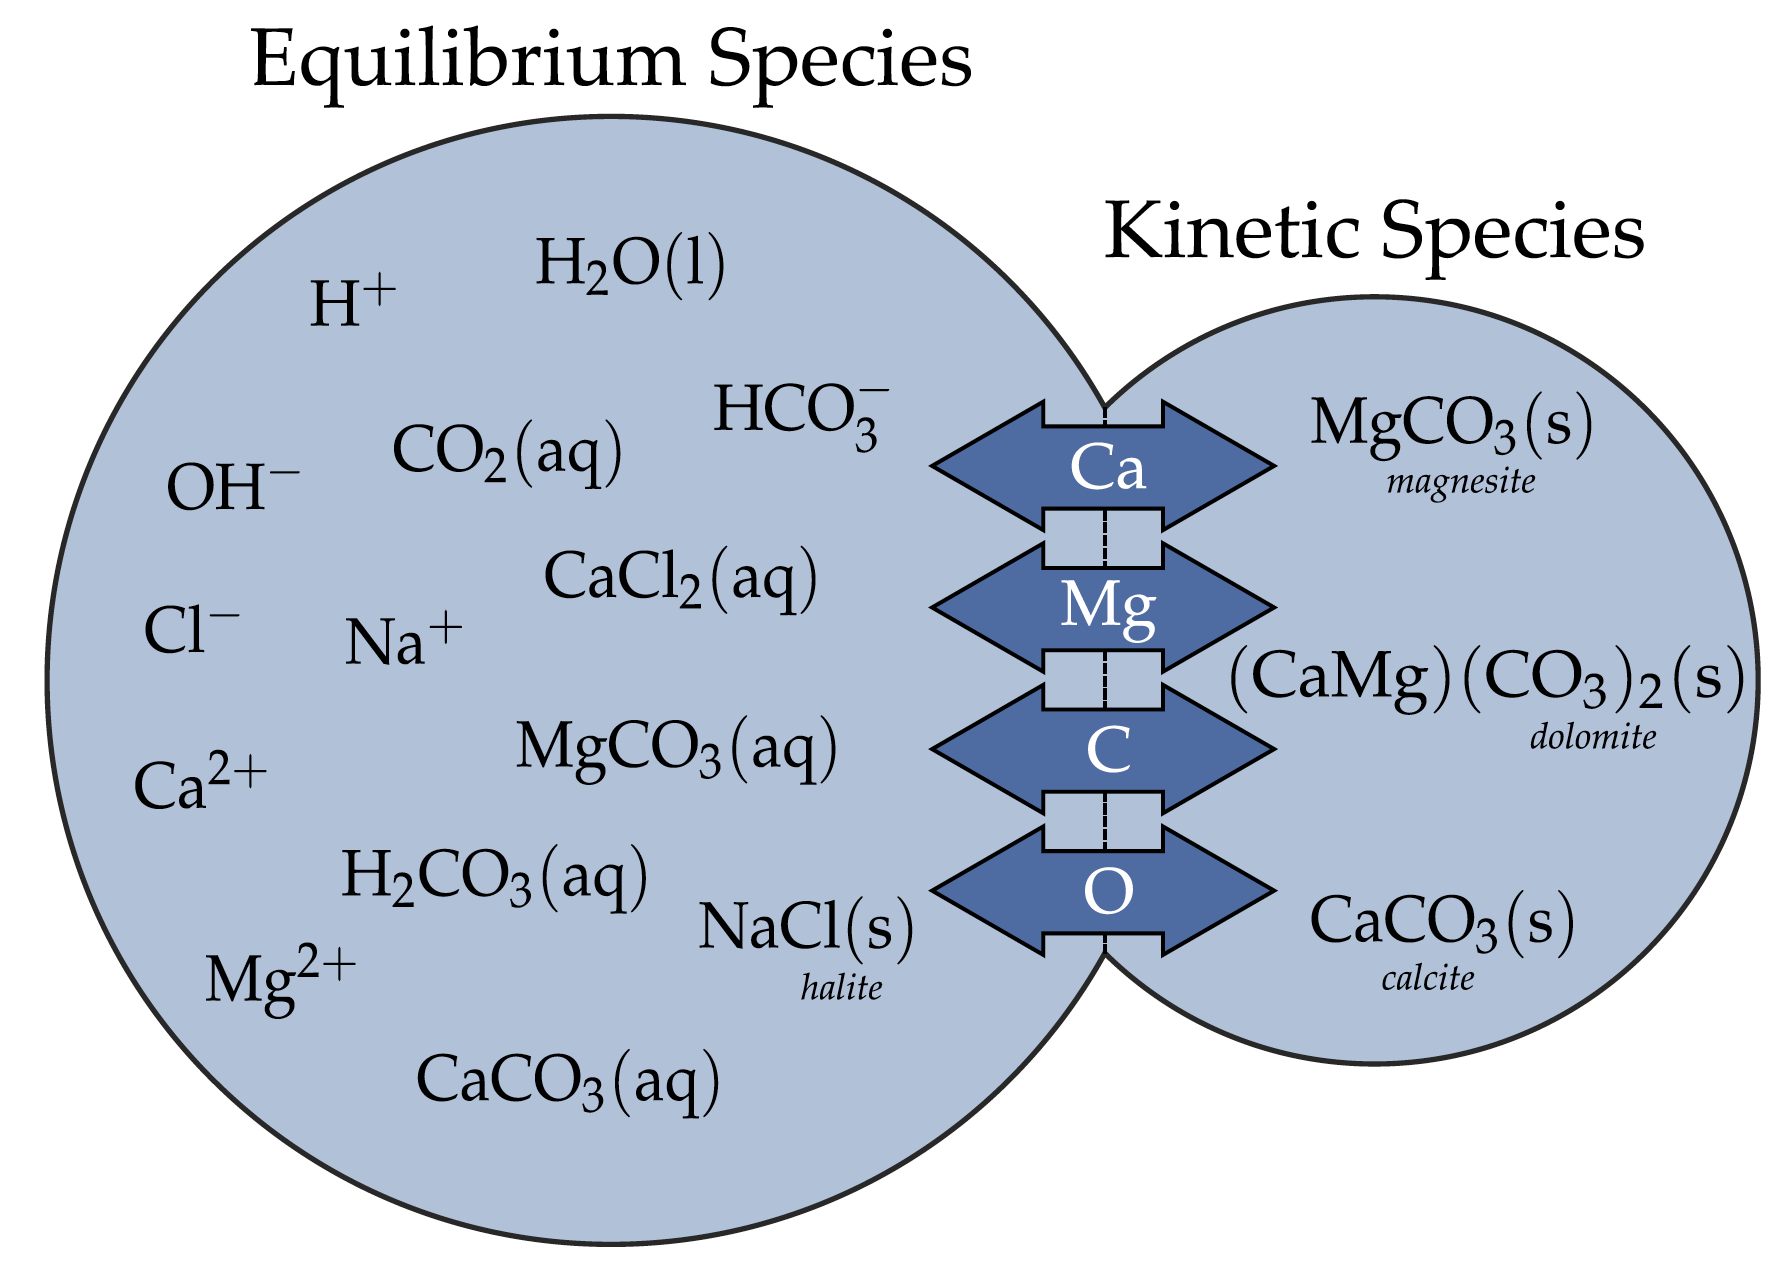
\includegraphics[height=0.7\textheight]{figures/chemical-kinetics/kinetic-equilibrium-element-exchange.png}
				\caption*{From A.M.M. Leal et al., Applied Geochemistry 55 (2015) 46--61.}
			\end{figure}
		\end{column}
	\end{columns}
\end{frame}
%
% --------------------------------------------------------------------------------------------------------------------%
% Equilibrium- and kinetically controlled system of ODE
% --------------------------------------------------------------------------------------------------------------------%
%
\begin{frame}{Equilibrium- and kinetically controlled system of ODE}
	%
	\begin{itemize}
		\item \alert{\bf Equilibrium- and kinetically-controlled reactions} requires the solution of the {\bf system of ODEs}
	\begin{alignat}{4}
		\frac{{d}b_{e}}{{d}t} & = f_e(n_{e}) & \qquad & t>0, & b_{e}=An_{e}^{\circ} & \qquad & t=0,\label{eq:kinetics}\\
		\frac{{d}n_{k}}{{d}t} & = f_k(n_{k}) &  & t>0, & \qquad n_{k}=n_{k}^{\circ} &  & t=0,\nonumber 
	\end{alignat}
	where 
	\begin{itemize}
		%\item $f_e$ is function of $A_{e}  \in \mathbb{R}^{E \times N_e} $ is the formula matrix of the equilibrium species, 
		%\item $r$ is the vector of \emph{rate}s \emph{(rate-functions)} of the kinetically-controlled reactions, 
%		\item $q_e, q_{k}$ denote the vector of \emph{inflow/outflow rates of the equilibrium and kinetic species},
		\item $n_{k}\in\mathbb{R}^{{N}_k}$ and $n_{e}\in\mathbb{R}^{{N}_e}$ are the amounts of the equilibrium and kinetic species,
		\item $n_{e}^{\circ}, n_{k}^{\circ}$ is vector of the \emph{initial amounts of the equilibrium and kinetic species}, respectively.
	\end{itemize}
	%
	\pause
	\item \alert{\bf How do we calculate $n_{e}$ after  $b_e$ is recovered by the system of ODEs}? 
	%
	\end{itemize}
\end{frame}
%
\begin{frame}{Chemical equilibrium calculation}
	\begin{itemize}
		\item To calculate $n_{e}$, we solve {\bf the fundamental GEM problem}
		%
		\[
		n_e 
		= \mathop{\mathrm{argmin}}_{n_{e}} G_{e} 
		= n_{e}^{{\rm T}}\mu_{e} \quad\mbox{s.t.} 
		\quad A_{e}n_{e}=b_{e},n_{e}\geq0.\]
		%
		\item Here, $\mu_{e,i} = \mu_{e,i}(T,P,n)\coloneqq\mu_{e,i}^{\circ}+RT\ln a_{e,i}$ denotes the {\bf chemical potential} of the $i$th species with 
		\begin{itemize}
		\item $R$ is the universal gas constant, 
		\item $\mu_{e,i}^{\circ}=\mu _{e,i}^{\circ}(T,P)$ the \emph{standard chemical potential} of the $i$th species, and
		\item $a_{e,i}=a_{e,i}(T,P,n)$ the \emph{activity} of the $i$th species.
		\end{itemize}
	\end{itemize}
	%
\end{frame}
%
% --------------------------------------------------------------------------------------------------------------------%
% Example, partition to kinetic and equilibrium species
% --------------------------------------------------------------------------------------------------------------------%
%
\begin{frame}{Example, Partition to kinetic and equilibrium species \, i}
	\begin{figure}
		\centering
		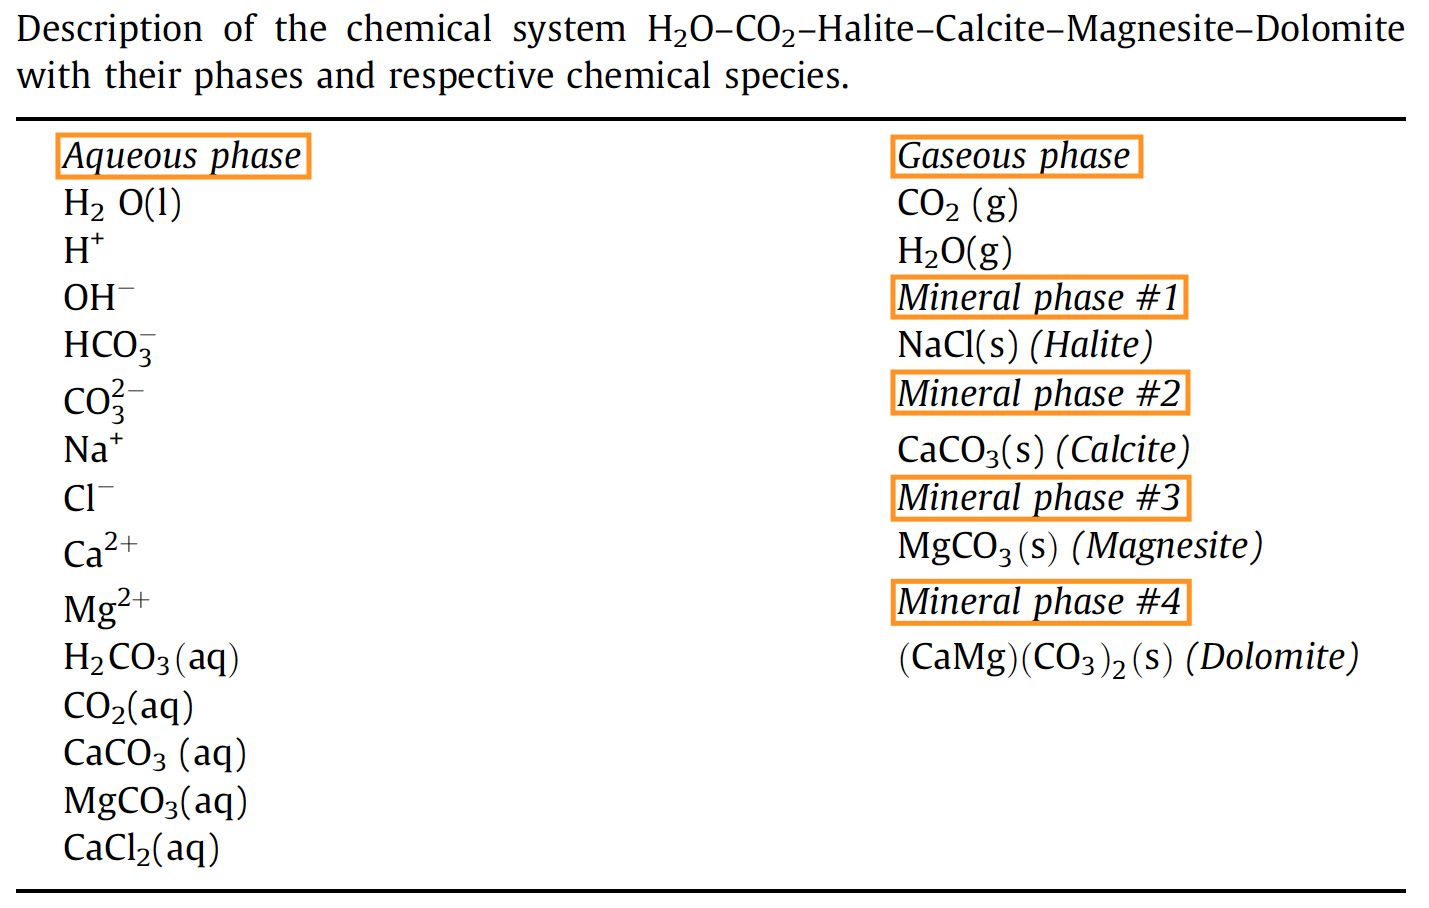
\includegraphics[height=0.85\textheight]{figures/chemical-kinetics/partitioning-example-1.png}
		\caption*{From A.M.M. Leal et al., Applied Geochemistry 55 (2015) 46--61.}
	\end{figure}
	%
\end{frame}
%
\begin{frame}{Example, Partition to kinetic and equilibrium species \, ii}
	\begin{figure}
		\centering
		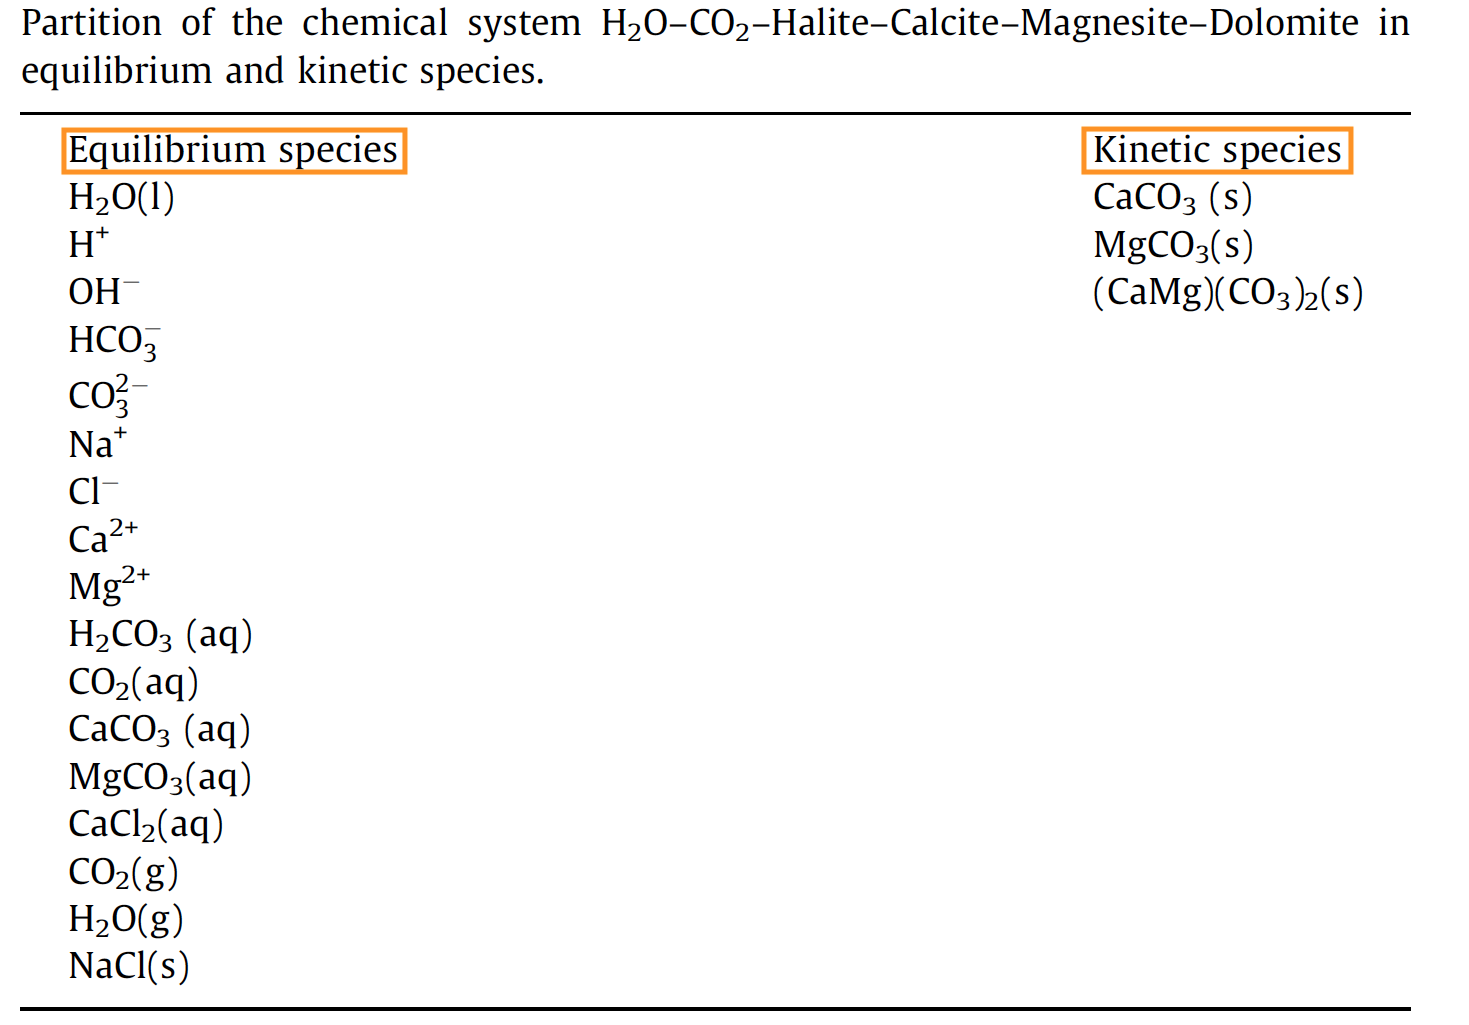
\includegraphics[height=0.85\textheight]{figures/chemical-kinetics/partitioning-example-2.png}
		\caption*{From A.M.M. Leal et al., Applied Geochemistry 55 (2015) 46--61.}
	\end{figure}
	%
\end{frame}
%
\begin{frame}{Example, Partition to kinetic and equilibrium species \, iii}
	\begin{figure}
		\centering
		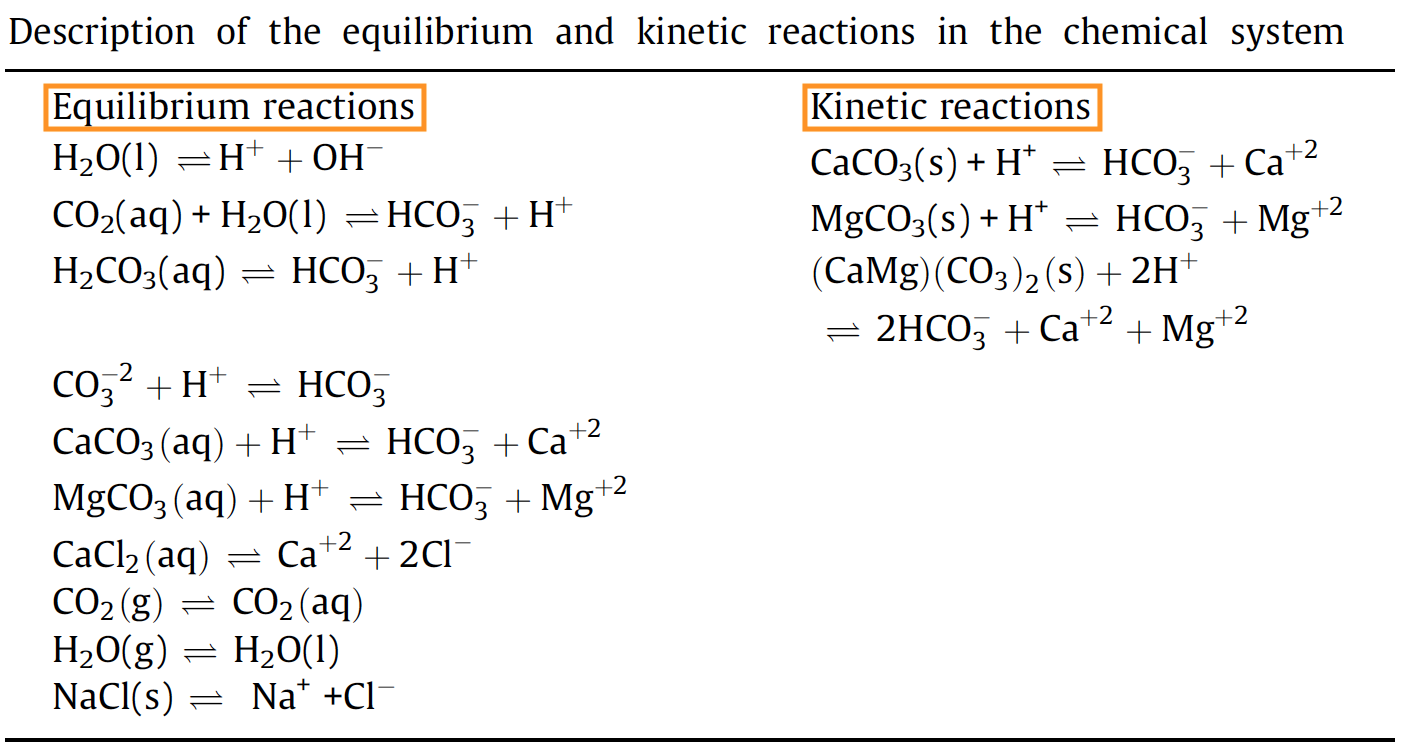
\includegraphics[height=0.85\textheight]{figures/chemical-kinetics/partitioning-example-3.png}
		\caption*{From A.M.M. Leal et al., Applied Geochemistry 55 (2015) 46--61.}
	\end{figure}
	%
\end{frame}
%
% --------------------------------------------------------------------------------------------------------------------%
% Differential-algebraic equations for equilibrium and kinetic chemical system
% --------------------------------------------------------------------------------------------------------------------%
%
\begin{frame}{Differential-algebraic equations for equilibrium and kinetic chemical system}
	\begin{itemize}
	\item The evolution of the chemical state of a system undergoing a
	{\bf mixed equilibrium and kinetic} process is governed by the following
	\alert{\bf differential-algebraic equations (DAE)}
	%
	\begin{alignat*}{4}
		\frac{\mathrm{d}b_{e}}{\mathrm{d}t} & = f_e(n_e)& \qquad & t>0, & b_{e}=An_{e}^{\circ} & \qquad & t=0,\label{eq:full-kinetics}\\
		\frac{\mathrm{d}n_{k}}{\mathrm{d}t} & = f_k(n_k) &  & t>0, & \qquad n_{k}=n_{k}^{\circ} &  & t=0,\nonumber \\
		n_{e} & =\varphi(T,P,b_{e}) &  & t>0. & &  & 
		\nonumber 
	\end{alignat*}
	%
	where $n^{\circ}=[n_{e}^{\circ},n_{k}^{\circ}]^{{\rm T}}$ is a given
	initial condition with provided on each time-step triple ($T,P,b_e)$.
	\end{itemize}
	%
\end{frame}
%
% --------------------------------------------------------------------------------------------------------------------%
% General rate law for mineral growth or dissolution
% --------------------------------------------------------------------------------------------------------------------%
%
\begin{frame}{General rate law for mineral growth or dissolution}
	\begin{itemize}
       \item In equation controlling kinetic species 
       %
       $$\frac{{\rm d} n_k}{{\rm d} t} = f_k(n_k) = \nu^{\rm T} r(n_k),$$
       %
       the \alert{\bf general rate law for mineral precipitation and dissolution} (Lasaga, 1981 and Palandri
       and Kharaka, 2004) can be formulated as
		%
		\[
		r_{j}(T,P, n):= S_{j}(n)\sum_{m} M_{j,m}(T,P,n),
		\]
		%
		where
		%
		\begin{itemize}
			\item $r_{j}:\mathbb{R}^{2+N}\rightarrow\text{\ensuremath{\mathbb{R}}}$ is a {\it rate function of the mineral} in the $j$th reaction,
			\item $S_{j} = S_{j}(n_j)$ is the corresponding {\it surface area function} of the mineral $[{\rm m^2}]$,
			\item $M_{j, m}$ is the {\it $m$-th kinetic mechanism} function of the mineral $[{\rm \tfrac{mol}{s \, m^2}}]$.
		\end{itemize}
%	\pause
%	 \item \alert{\bf Mineral surface areas $A_{j} = A_{j}(n_j)$} is also a function of kinetic species amounts.
%	 can evolve based on two models:
%	 %
%	 \begin{itemize}
%	 	\item {\bf linear dependence} on the amount of mineral $n_{j}$, i.e., $A_{j}:=n_{j} \sigma_{j}$ with $\sigma_{j}$ being constant specific surface area, or 
%	 	\item {\bf fractional dependence}, i.e.,  $A_{j}:=A_{j}^{\circ}\Big(\tfrac{n_{j}}{n_{j}^{\circ}}\Big)^{2/3}$, where 
%	 	$A_{j}^{\circ}$ is the \emph{initial surface area of the mineral} and $n_{j}^{\circ}$ is the \emph{initial number of moles of the mineral}.
%	 \end{itemize}
	\end{itemize}

\end{frame}	
%
% --------------------------------------------------------------------------------------------------------------------%
% Kinetic mechanism function
% --------------------------------------------------------------------------------------------------------------------%
%
\begin{frame}{Kinetic mechanism function}
	\begin{itemize}
		\item \alert{\bf Kinetic mechanism function} of the mineral includes in $k_{j,m}$ different scenarios (such as acid, neutral, base, carbonate,etc) and is defined as
		%
		\[
		M_{j,m}:= k_{j,m} \, {\rm sgn}(1-\mathrm{SI})\, 
		|1-\mathrm{SI}^{p_{m}}|^{q_m}\,C_{j, m},
		\]
		%
		where
		%
		\begin{itemize}
			\item $\mathrm{SI}$ is the \emph{saturation index} of the $j$th mineral, 
			\item $p_{i}$ and $q_{i}$ are \emph{empirical exponents} used to fit the rate law,
			\item $C_{j,m}$ is a function to model \emph{catalysts and inhibitors} of the mineral reaction, 
			\item 
			%
			\[
			k_{j,m}:=k_{j,m}^{\circ} e^{\Big[-\tfrac{E_{m,i}}{R}\Big(\tfrac{1}{T}-\tfrac{1}{298.15}\Big)\Big]} \]
			%
			is the \emph{\bf rate constant} of the mineral reaction (according to the \emph{\bf Arrhenius equation}) with
			\begin{itemize}
				\item $k_{j,m}^{\circ}$ as the \emph{reaction rate} constant at 25 °C, 
				\item $E_{j,m}$ as the \emph{activation energy}, 
				\item $R$ as the \emph{universal gas constant} and T as the given temperature, 
			\end{itemize}
		\end{itemize}
%	\pause
%	\item The \alert{\bf kinetic mineral mechanisms} includes in $k_{j,m}$ different scenarios such as acid, neutral, base, carbonate, etc.
	\end{itemize}
\end{frame}
%
% --------------------------------------------------------------------------------------------------------------------%
% Example, Barite precipitation using Palandri and Kharaka parameters
% --------------------------------------------------------------------------------------------------------------------%
%
% \begin{frame}[fragile]{Example of barite precipitation using acidic mechanism}
% 	\small 
% 	%
% 		In rate law $r_{\sf Barite} = S \, {\rm sgn}(1-\mathrm{SI})\, |1-\mathrm{SI}| \, 
% 		k \, e^{\Big[-\tfrac{E_a}{R}\Big(\tfrac{1}{T}-\tfrac{1}{298.15}\Big)\Big]},$ 
% 		we defined 
% 		$S$, $k$, and $E_a$:\\[10pt]	
% 			%
% \begin{lstlisting}[language=Python, caption=Define barite mineral reaction and its parameters]
% eq_str_barite = "Barite = SO4-- + Ba++"
% min_reaction_barite = editor.addMineralReaction("Barite") \
% 	.setEquation(eq_str_barite) \
% 	.addMechanism("logk = -8.6615 mol/(m2*s); Ea = 22 kJ/mol") \
% 	.setSpecificSurfaceArea(0.006, "m2/g")
% \end{lstlisting}
% 	\begin{figure}
% 		\centering
% 		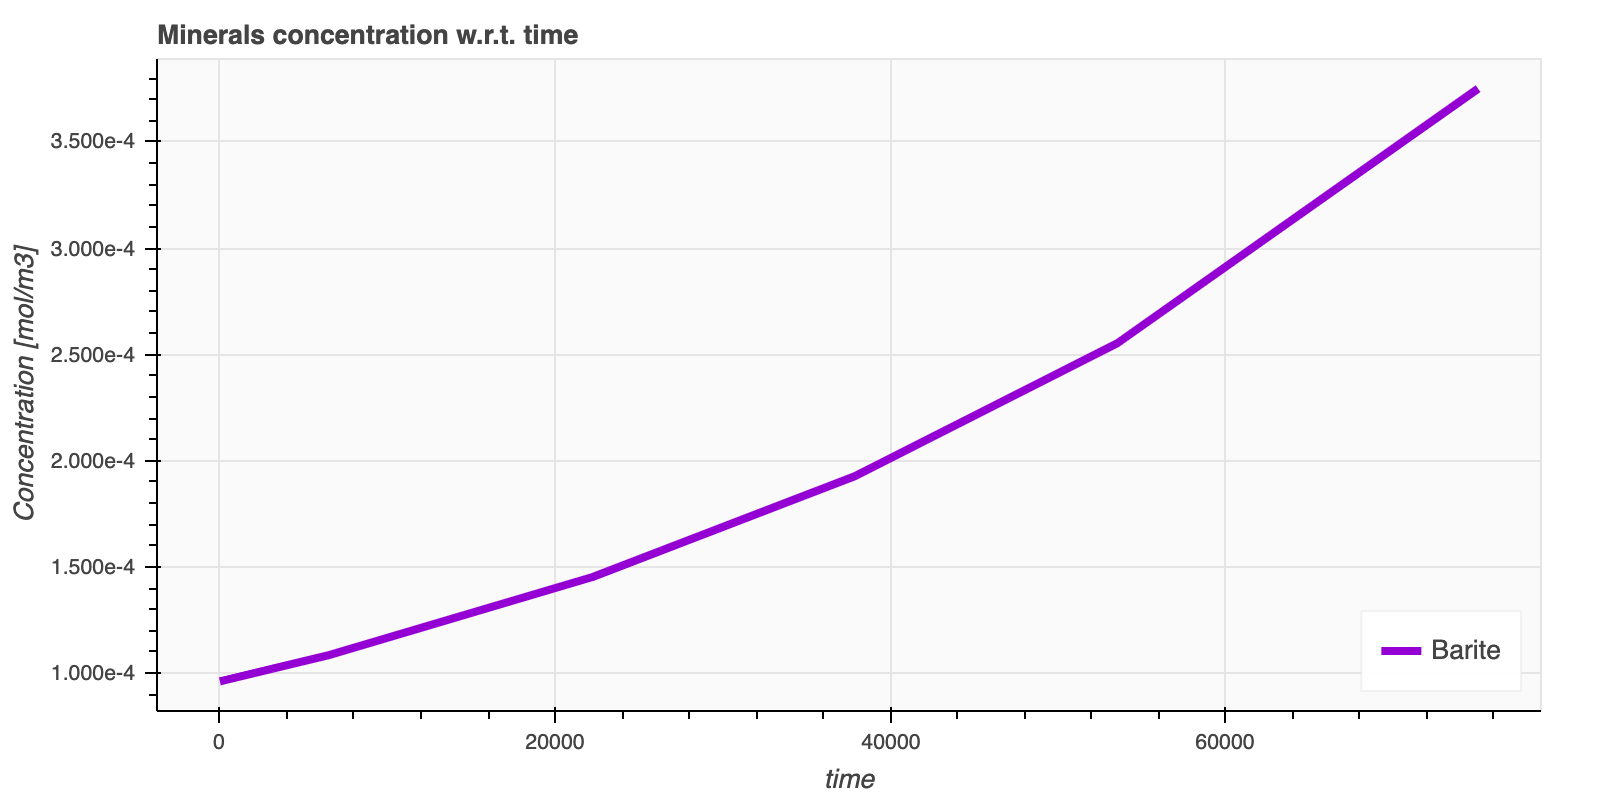
\includegraphics[height=0.37\textheight]{figures/chemical-kinetics/barite-acidic-mechanism.png}
% 		\caption*{Barite precipitation.}
% 	\end{figure}
% \end{frame}
%
% --------------------------------------------------------------------------------------------------------------------%
% Example, Barite precipitation using alternative database
% --------------------------------------------------------------------------------------------------------------------%
%
%\begin{frame}[fragile]{Example of barite precipitation using alternative database}
%	
%	\begin{itemize}
%		\item More realistic \alert{\bf mechanism:} 
%		
%		\[
%		r_{m}:=n_{m}\,S_{m}\,M_{m}\:k_{pre}\,(1-\ensuremath{\Omega}),\quad\mbox{where}\quad k_{pre}:=\mbox{{-2.18e-9}}\cdot\exp\Big[-\tfrac{22}{R}\Big(\tfrac{1}{T}-\tfrac{1}{298.15}\Big)\Big]\cdot10^{0.6\sqrt{I}},
%		\]
%	\end{itemize}
%	
%	\begin{figure}
%		\centering
%		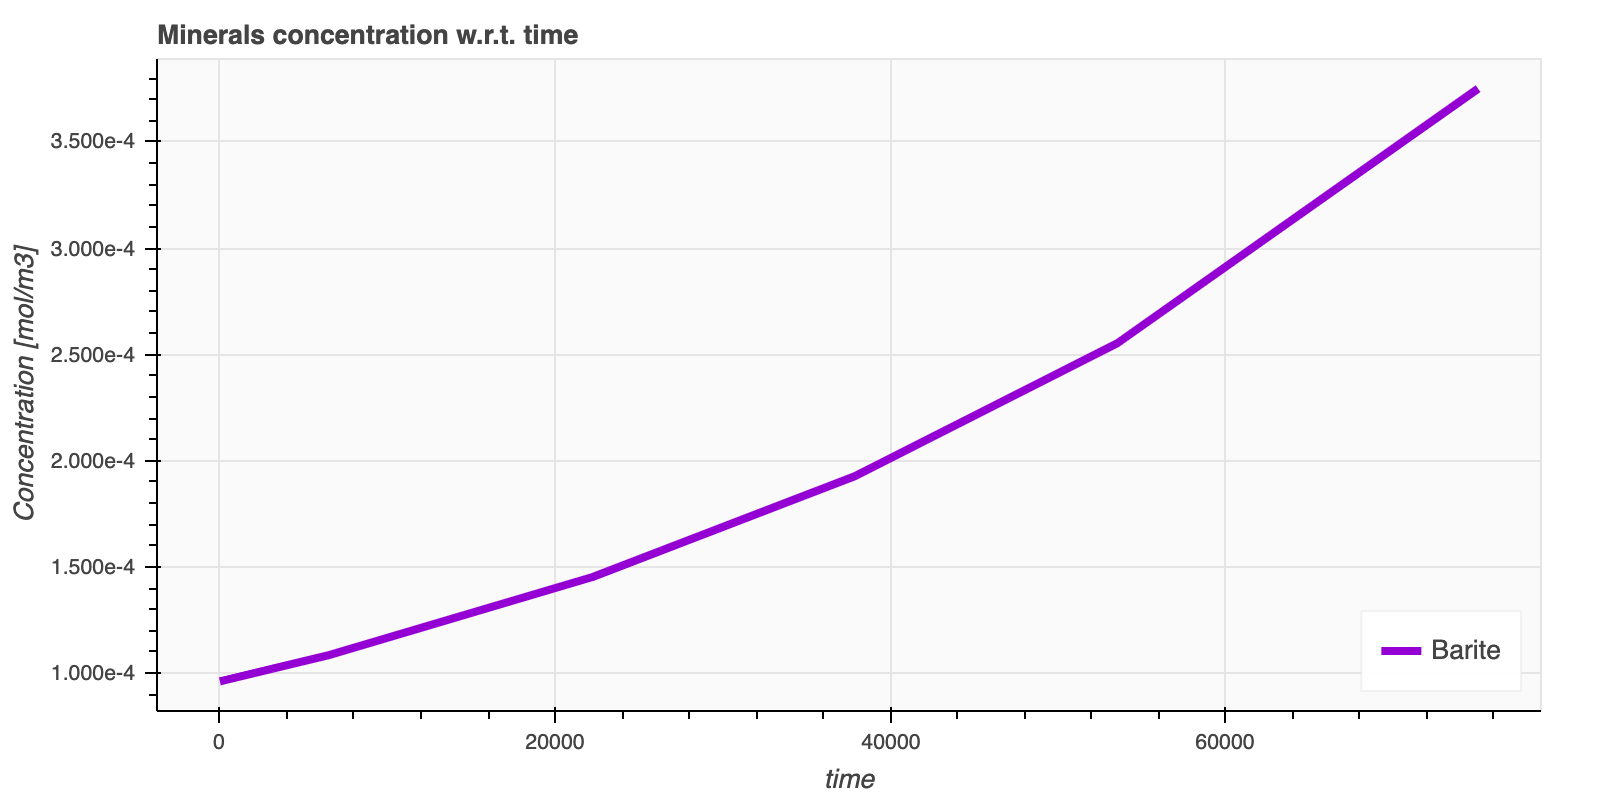
\includegraphics[height=0.55\textheight]{figures/chemical-kinetics/barite-acidic-mechanism.png}
%		\caption*{\alert{TODO: Generate correct pictures with workstations!} More realistic barite precipitation.}
%	\end{figure}
%	
%\end{frame}
%
% --------------------------------------------------------------------------------------------------------------------%
% Example, Souring with hematite
% --------------------------------------------------------------------------------------------------------------------%
%
\begin{frame}[fragile]{Example of hematite kinetic mechanisms in reservoir souring}
	\small
\alert{\bf Hematite} mineral reacts according to the reaction 
	\[\mathsf{Fe_{2}O_{3}(hematite)+6\,H^{+}=3\,H_{2}O(l)+2\,Fe^{3+}}\]
	and has the following kinetic rate dependent on neutral, acidic, and sulfide promoted mechanisms:
	%
	\[
	\begin{array}{ll}
		r_{\sf Hematite}:=n \,S\,M\,\bigg(\frac{n}{n^\circ}\bigg)^{2/3}\: & k_{\rm diss}\,(1-\ensuremath{\Omega}), \\
		&  k_{\rm diss}:=k_{\rm neu}+k_{\rm acid}+k_{\rm sulfide},\\
		& k_{\rm neu}:=\mbox{2.51e-15}\cdot e^{\Big[-\tfrac{66.2}{R}\Big(\tfrac{1}{T}-\tfrac{1}{298.15}\Big)\Big]},\\
		& k_{\rm acid}:=\mbox{4.07e-10}\cdot e^{\Big[-\tfrac{66.2}{R}\Big(\tfrac{1}{T}-\tfrac{1}{298.15}\Big)\Big]}\cdot a({\rm H^{+}}),\\
		& k_{\rm sulfide}:=\mbox{3.5e-9}\cdot e^{\Big[-\tfrac{40}{R}\Big(\tfrac{1}{T}-\tfrac{1}{298.15}\Big)\Big]}\cdot a^{1/2}({\rm HS^{-}}),
	\end{array}
	\]
	where $M$ is the molar mass.
\end{frame}

\section{Numerical method for chemical kinetics calculation}
%
% --------------------------------------------------------------------------------------------------------------------%
% History of stiffness of system of ODEs
% --------------------------------------------------------------------------------------------------------------------%
%
\begin{frame}{History of stiffness of system of ODEs}
	\begin{itemize}
		\item \alert{\bf Stiffness} is the characteristics of {\bf ``how hard'' is it to solve a system of ODEs}. 
		%
		\pause
		\item The first identification due to chemical engineers 
		Curtiss and Hirschfelder (1952):\\[-20pt]
		\begin{multline*}
			\text{\emph{``Stiff equations are equations where certain implicit methods perform better, }} \\ 
			\text{\emph{usually tremendously better, than explicit ones''.}}
		\end{multline*}
		\vskip -10pt
		\pause
		\item \alert{\bf It comes from} the system of coupled equations for combustion has very different time scale characteristics. In geochemistry, the situation is similar, but a little less critical. 
%		\item In particular, in Arrhenius equations the term 
%		%
%		\[
%		k_{j,m}:=k_{j,m}^{\circ} e^{\Big[-\tfrac{E_{m,i}}{R}(\tfrac{1}{T}-\tfrac{1}{298.15})\Big]} \]
%		%
%		contributes into
	\pause
		\item If {\bf nonstiff methods} are employed to solve stiff problems $\Rightarrow$ {\bf more computational effort is required}.
		%
		\pause
		\item This results in {\bf chemical problems being a bottleneck} in reaction kinetics (and other areas, e.g.,  electrical engineering, mechanical engineering, etc.) for 15 years.
		%
		\pause
		\item But, in 1968, a variety of methods began to appear in the literature.
	\end{itemize}
\end{frame}
%
% --------------------------------------------------------------------------------------------------------------------%
% Example of stiff problem and complication by numerical integration
% --------------------------------------------------------------------------------------------------------------------%
%
\begin{frame}{Example of stiff problem and complication by numerical integration}
	\small
	\begin{itemize}
		\item The \alert{\bf stiff equations and systems}: 
		let $\epsilon >$ 0 be a small small parameter and  consider the {\bf initial value problem}
		%
		\[
		\tfrac{{d} x(t)}{{d} t} = - \tfrac{1}{\epsilon}\,x(t), \quad 
		x(0) = 1, \quad t \in [0, T],
		\]
		%
		with the \alert{\bf exponential solution} is $x(t) = e^{-\tfrac{t}{\epsilon}}$.
		\pause
		\item In order to accurately integrate this problem with Euler method, {\bf $\Delta t$ (integration time steps) must be smaller than $\epsilon$}.
	\end{itemize}
	\begin{figure}[!t]
		\centering
		\subfloat[]{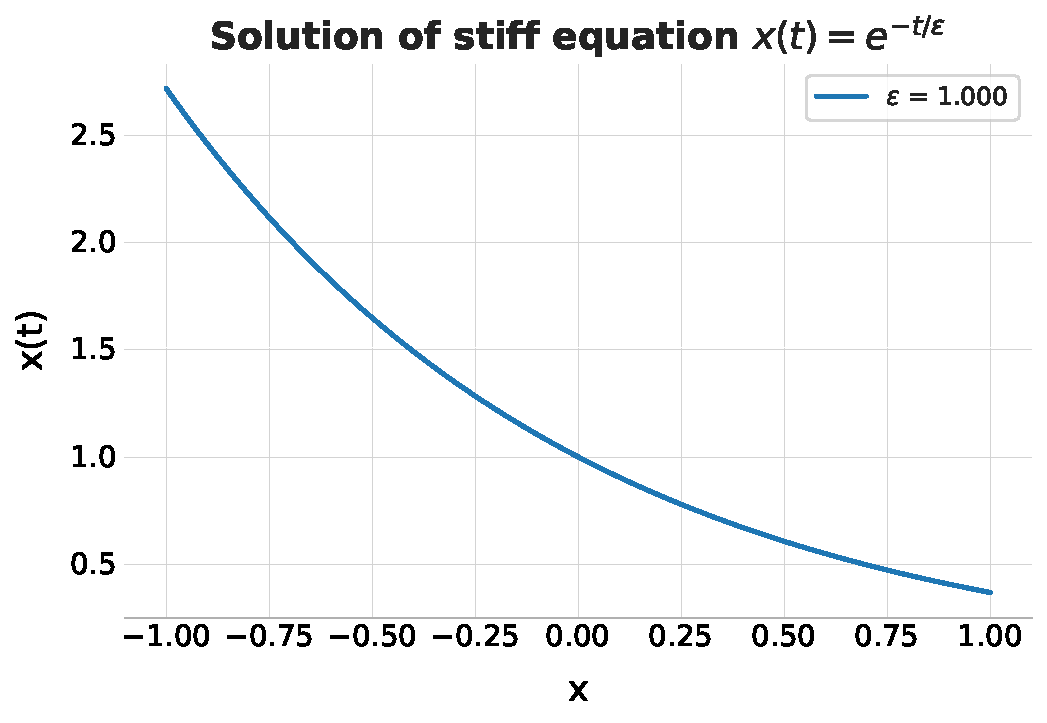
\includegraphics[width=0.3\textwidth]{figures/chemical-kinetics/solution-stiff-odes-eps-1}} \;
		\subfloat[]{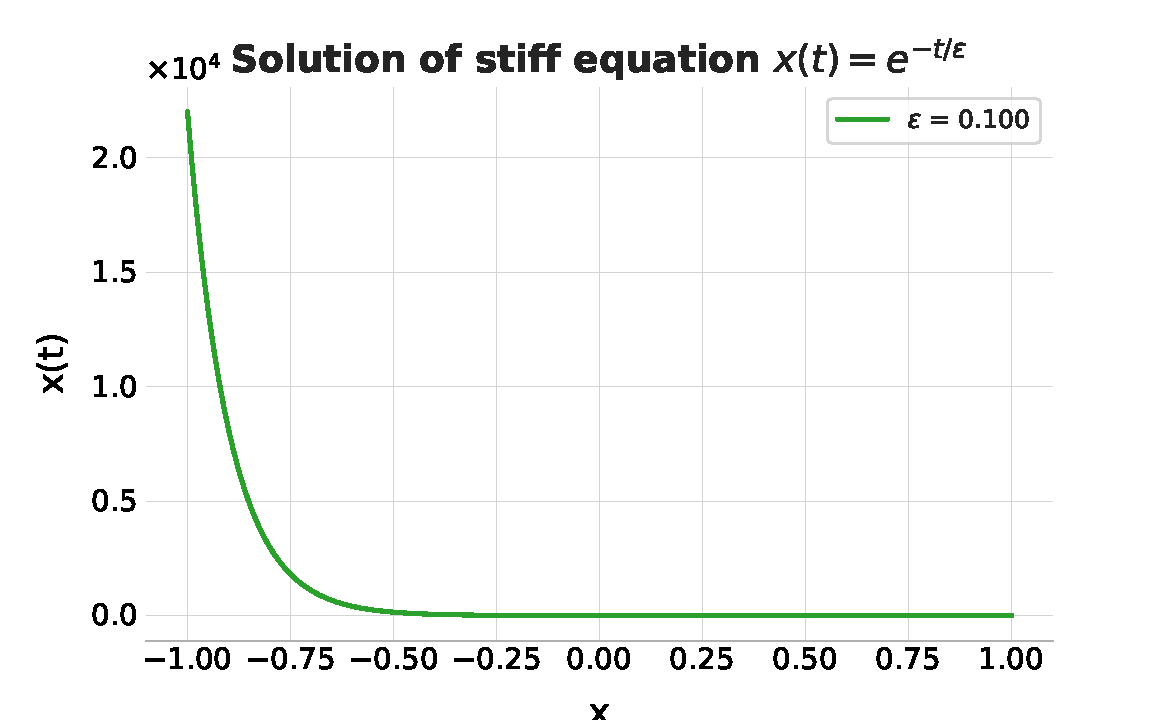
\includegraphics[width=0.35\textwidth]{figures/chemical-kinetics/solution-stiff-odes-eps-2}} \;
		\subfloat[]{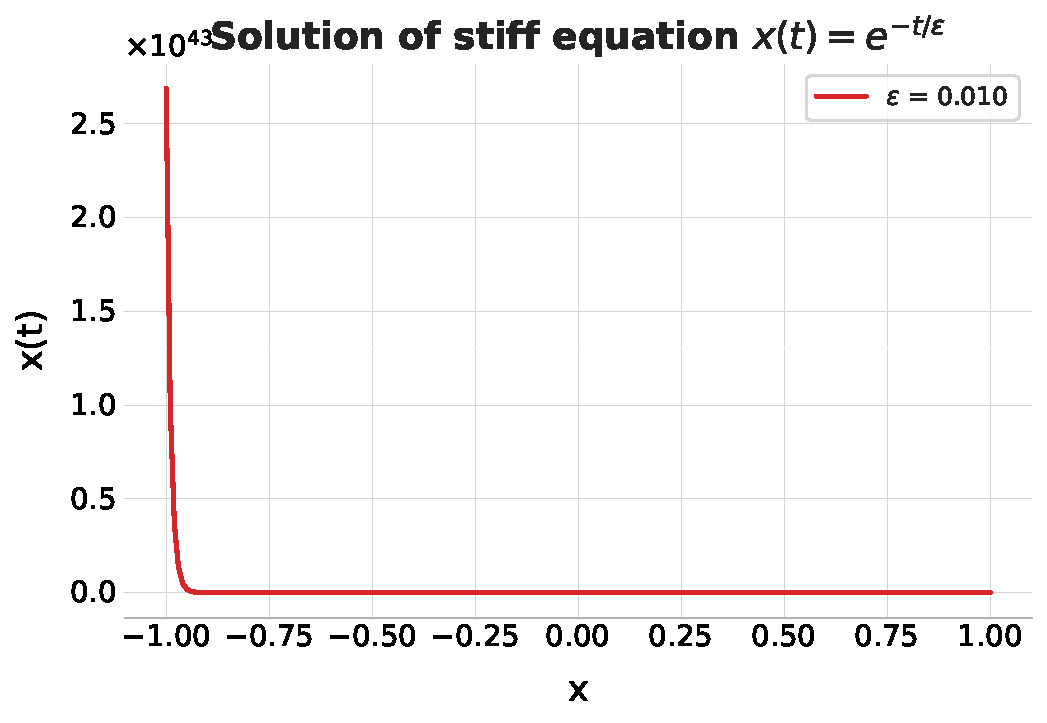
\includegraphics[width=0.3\textwidth]{figures/chemical-kinetics/solution-stiff-odes-eps-3}}
	\end{figure}
\end{frame}
%%
%% --------------------------------------------------------------------------------------------------------------------%
%% Stiffness of system of ODEs
%% --------------------------------------------------------------------------------------------------------------------%
%%
%\begin{frame}{History of stiffness of system of ODEs}
%	\begin{itemize}
%		\item The history of stiff differential equations goes back 55 years.
%		%
%		\item The first identification due to chemical engineers in 1952 (Curtiss and Hirschfelder, Proc. of the National Academy of Sciences of U.S., 1952): \\
%		\begin{multline*}
%			\text{\emph{``Stiff equations are equations where certain implicit methods perform better, }} \\ 
%			\text{\emph{usually tremendously better, than explicit ones''.}}
%		\end{multline*}
%		%
%		\item For 15 years, chemical problems a bottleneck in reaction kinetics and other areas, such as electrical engineering, mechanical engineering, etc,.
%		%
%		 \item In 1968, when a variety of methods began to appear in the literature.
%	\end{itemize}
%\end{frame}
%
% --------------------------------------------------------------------------------------------------------------------%
% Numerical integration schemes and codes for stiff systems
% --------------------------------------------------------------------------------------------------------------------%
%
\begin{frame}{Numerical integration schemes and codes for stiff systems}

\begin{itemize}

\item \alert{\bf One-step methods}:
%
\begin{itemize}
	\item implicit Runge-Kutta methods,
	\begin{itemize}
		\item e.g., Gauss, Radau, Lobatto methods, etc.
	\end{itemize}
	\item Rosenbrock methods (semi-implicit / semi-explicit / generalized / adaptive / additive Runge-Kutta methods),
	\item semi-implicit extrapolation methods, 
	%\item Implicit multistep BDF algorithm (Ascher and Petzold,
\end{itemize}
%
\item \alert{\bf Multi-step methods} (the first numerical methods to be proposed for stiff differential equations):
%
\begin{itemize}
	\item explicit Adams methods,
	\item predictor-corrector schemes,
	\item Nystrom methods, 
	\item backward differentiation formular (BDF) schemes.
\end{itemize}
%
\item For more details, see \cite{Hairer2010}.
%
\item In Reaktoro, for the integration of the chemical kinetics, the {\bf CVODE package implementing BDF methods} \cite{Cohen1996, Hindmarsh2005} is used. 
\end{itemize}

\end{frame}
%
% --------------------------------------------------------------------------------------------------------------------%
% Example, Roberts system
% --------------------------------------------------------------------------------------------------------------------%
%
\begin{frame}{Example, Roberts system}
	\vskip 10pt
	\small 
	%\begin{itemize}
		%\item 
		Consider the Roberts system modeling  \alert{\bf 3-species chemical kinetics problem}: 
		find amount $n = [n_{\mathsf{A}}, n_{\mathsf{B}}, n_{\mathsf{C}}]^{\mathrm{T}}$ 
		on the time-interval $t \in [0, 4 \cdot 10^{3}]$ with
		%
		\begin{itemize}
			\item reaction rates $k_a = 4 \cdot10^{-2}$, $k_b = 10^{4}$, $k_c = 3\cdot10^{7}$ and 
			\item initial condition $n^\circ = [n_\mathsf{A}^{\circ}, n_\mathsf{B}^{\circ}, n_\mathsf{C}^{\circ}]=[1, 0, 0]$.
		\end{itemize}
		%
		\vskip -10pt
		
		\begin{columns}[t]
			\column{.4\textwidth}
			% 
			   \footnotesize
				\begin{alignat*}{3}
					\mathsf{A} & \xrightleftharpoons[]{k_a} \mathsf{B} & \text{(slow)}\\[-5pt]
					\mathsf{B + C} & \xrightleftharpoons[]{k_b} \mathsf{A + C} & \text{(fast)}\\[-5pt]
					\mathsf{B + B} &\xrightleftharpoons[]{k_c} \mathsf{C + B} & \quad \text{(very fast)}
				\end{alignat*}
				%
				\qquad resulting in the system of ODEs
				$$
				\quad 
				\begin{cases}
					\tfrac{{\rm d} n_\mathsf{A}}{{\rm d} t} = - k_a\, n_\mathsf{A} + k_b\, n_\mathsf{B}\, n_\mathsf{C}\\
					\tfrac{{\rm d} n_\mathsf{B}}{{\rm d} t} =   k_a\, n_\mathsf{A}-k_b\, n_\mathsf{B}\, n_\mathsf{C}-k_c\, n_\mathsf{B}^{2}\\
					\tfrac{{\rm d} n_\mathsf{B}}{{\rm d} t} =   k_c\, n_\mathsf{B}^{2}
				\end{cases}
				$$
			\column{.6\textwidth}
			\vskip -5pt
			\begin{figure}[!h]
				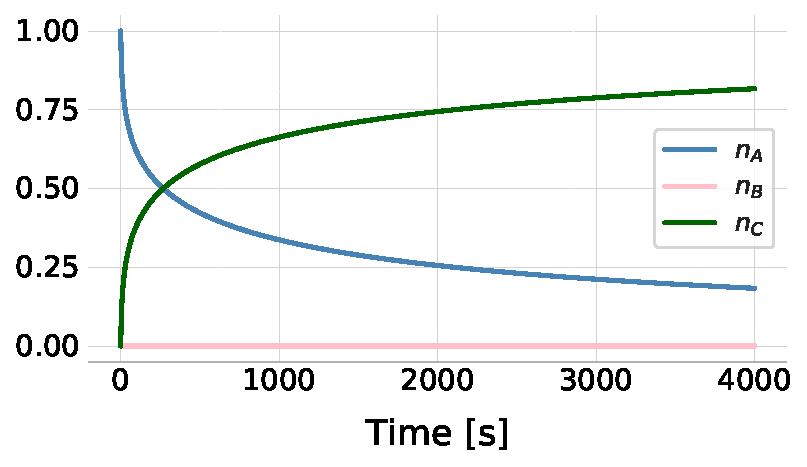
\includegraphics[width=0.75\textwidth]{figures/chemical-kinetics/approximations}
				\caption{\scriptsize Solution of the Roberts system.}
			\end{figure}
		\end{columns}
		%
		\vskip 5pt
		\textbf{Source code}: \href{https://polybox.ethz.ch/index.php/s/vZ54CLT6rooxoJ8}{\textcolor{indigo(dye)}{\it polybox}} using \href{https://docs.scipy.org/doc/scipy/reference/generated/scipy.integrate.odeint.html}{\textcolor{indigo(dye)}{odeint}} function of 
		\href{https://docs.scipy.org/doc/scipy/reference/integrate.html}{\textcolor{indigo(dye)}{\bf scipy.integrate}} Python package.
	%\end{itemize}
\end{frame}
%
% --------------------------------------------------------------------------------------------------------------------%
% Example,Kinetic dissolution of carbonates
% --------------------------------------------------------------------------------------------------------------------%
%
\begin{frame}{Example, Calcite dissolution}
	
 Jupyter notebook tutorial \href{https://github.com/mtsveta/reaktoro-jupyter/blob/geofluids-examples/tutorial/eq.sodium-chloride-solubility-in-water.ipynb}{\textcolor{indigo(dye)}{\it Kinetic dissolution of carbonate}} (with Reaktoro v1) with \href{https://polybox.ethz.ch/index.php/s/DEVT1vjNEJNh4Zo}{\textcolor{indigo(dye)}{\it recording}}:
 	%
 	\begin{figure}[!t]
 	\centering
 	\subfloat[Calcite dissolution]{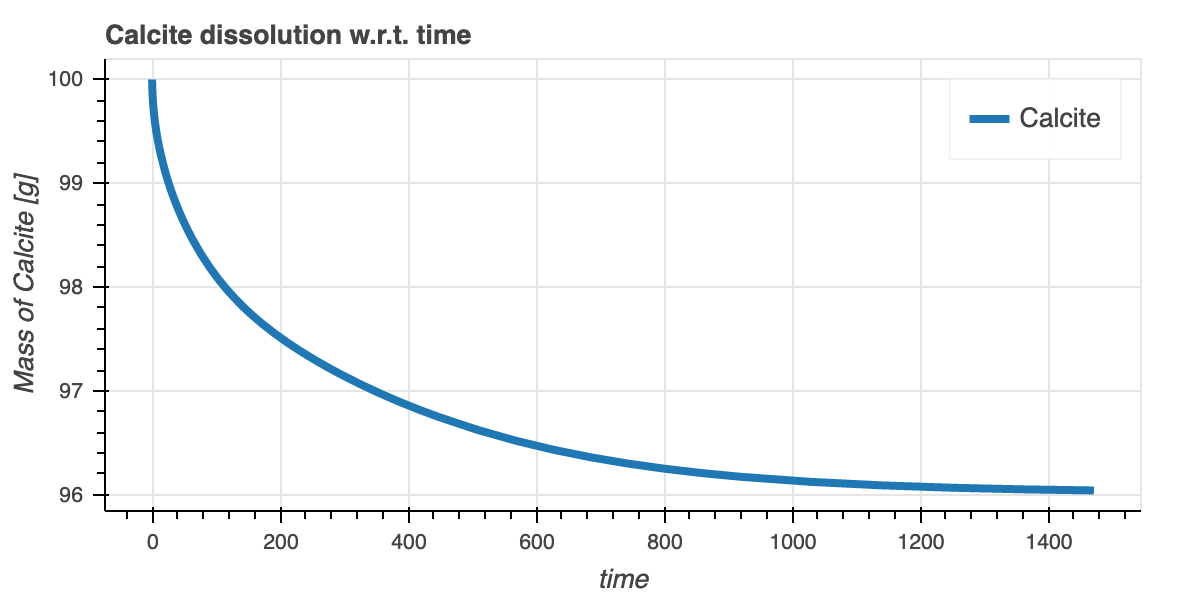
\includegraphics[width=0.35\textwidth]{figures/chemical-kinetics/kinetic-tutorial-calcite.png}} \qquad \qquad
 	\subfloat[Dolomite dissolution]{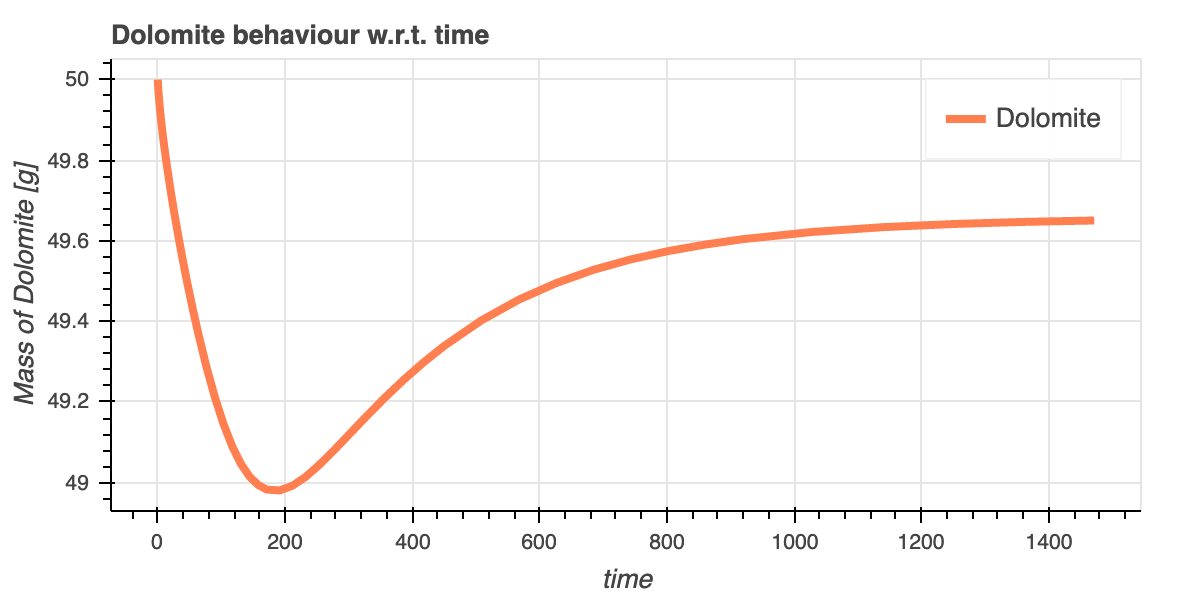
\includegraphics[width=0.35\textwidth]{figures/chemical-kinetics/kinetic-tutorial-dolomite.png}} \\[5pt]
 	\subfloat[$\mathsf{Ca^{2+}}$ and $\mathsf{Mg^{2+}}$ molality increase]{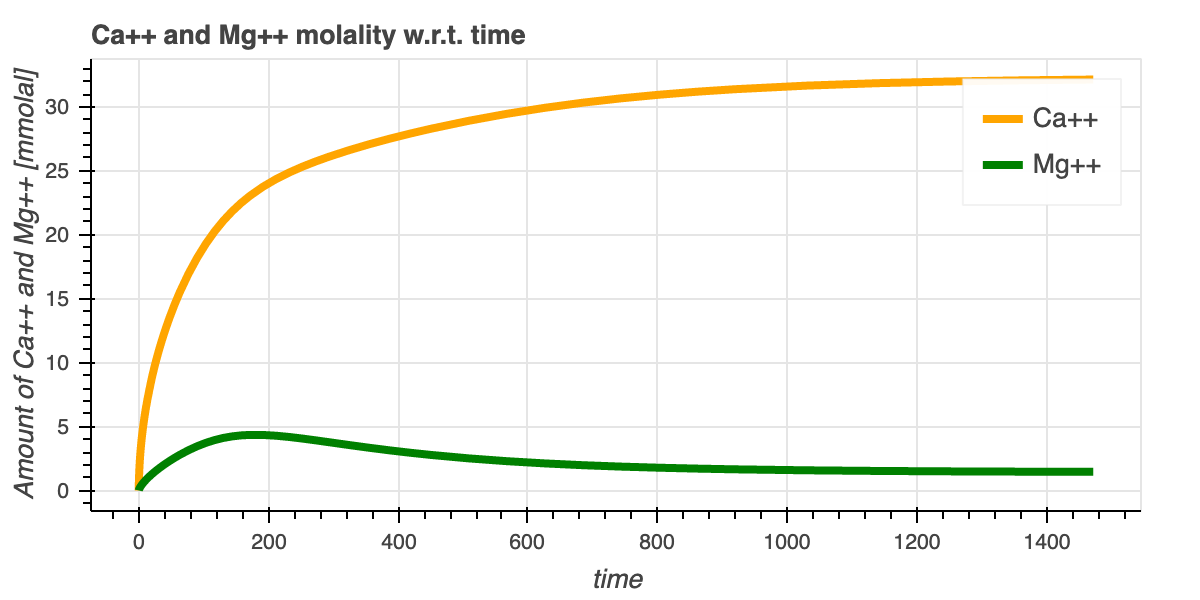
\includegraphics[width=0.35\textwidth]{figures/chemical-kinetics/kinetic-tutorial-ca-mg-ions.png}} \qquad \qquad
 	\subfloat[pH]{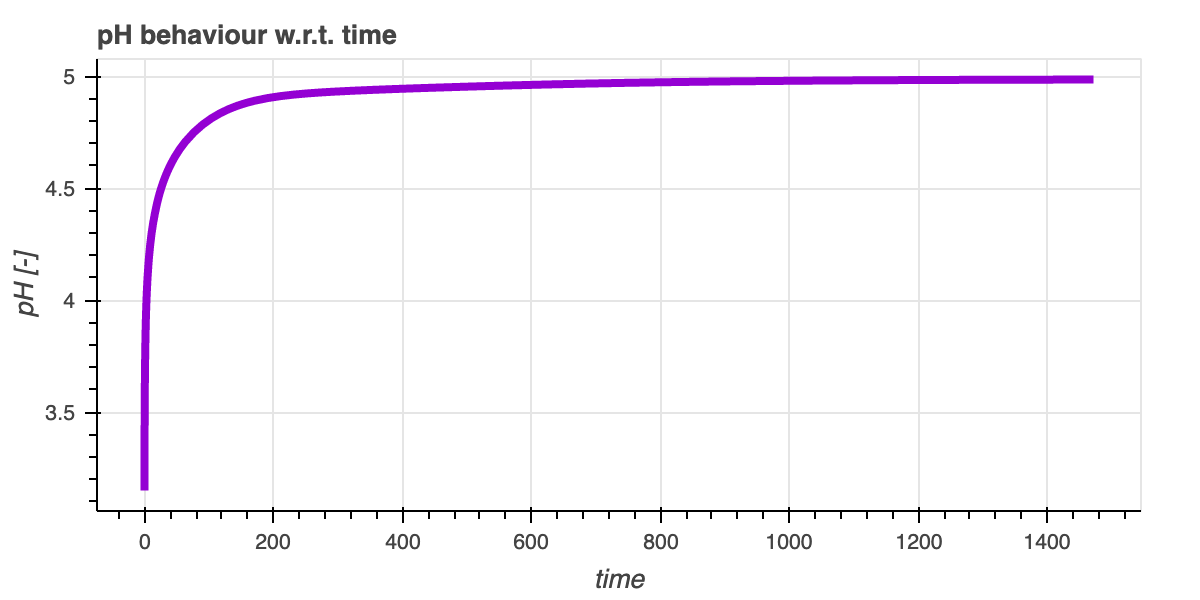
\includegraphics[width=0.35\textwidth]{figures/chemical-kinetics/kinetic-tutorial-ph.png}}
 	%
 \end{figure}
 
	
\end{frame}